\documentclass[10pt,a4paper,parskip=half]{scrreprt}
%\documentclass[10pt,a4paper, draft]{scrreprt}
\usepackage[utf8]{inputenc}
\usepackage[ngerman]{babel}
\usepackage{amsmath}
\usepackage{amsfonts}
\usepackage{amssymb}
\usepackage{dsfont}
\usepackage[framemethod=tikz]{mdframed} % sollte nach amsmath geladen werden
\usepackage{esvect}
\usepackage{geometry}
\usepackage{graphicx}
%\renewcommand*\includegraphics[2][]{} % einkommentieren um alle Bilder auszublenden
\usepackage{wrapfig} % Um Bilder einzubinden, die vom Text umflossen sind
\usepackage{placeins} % float barrier
\usepackage[german, intoc, refpage]{nomencl}
\usepackage{listings}
\usepackage{todonotes}
\usepackage{abraces} % Benutzerdef. Klammern
\usepackage{algorithmicx}
\usepackage{algorithm}
\usepackage[noend]{algpseudocode}
\usepackage{blindtext} % dient zum generieren von Blindtext für Testzwecke
\usepackage{hyperref} %das muss zu letzt geladen werden



\geometry{a4paper,left=35mm,right=35mm} % Einstellen der Seitenränder

\pagestyle{headings}

\setlength{\parindent}{1em} % Setzt den Wert für Einzug bei einem neuen Absatz

\floatname{algorithm}{Algorithmus} % ändert algorithm in Algorithmus ab.
\addto\captionsngerman{ % Zum Ändern automatisch generierter Bezeichner wie "Abbildung" in figure-Umgebung
    \renewcommand{\figurename}{Abb.}
  %  \renewcommand{\tablename}{Tab.}
}


\mdfdefinestyle{mystyle}{
    linecolor=gray!20,linewidth=3pt,
    frametitlerule=true,
    frametitlebackgroundcolor=gray!20,
    roundcorner=1pt,
    innertopmargin=\topskip,
}
\newmdenv[style=mystyle, frametitle=Quelldateien]{quell}


% --- Abkürzungsverzeichnis: ----------------------------
% START % Näheres siehe http://my.opera.com/timomeinen/blog/show.dml/68644
% Befehl umbenennen in abk
\let\abk\nomenclature
% Deutsche Überschrift
\renewcommand{\nomname}{Abkürzungsverzeichnis}
% Punkte zw. Abkürzung und Erklärung
\setlength{\nomlabelwidth}{.20\hsize}
\renewcommand{\nomlabel}[1]{#1 \dotfill}
% Zeilenabstände verkleinern
\setlength{\nomitemsep}{-\parsep}
\makenomenclature



%% Hier beginnt das eigentliche Dokument
\begin{document}

\begin{titlepage}

\title{Implementation of a raytracer
\begin{center}
   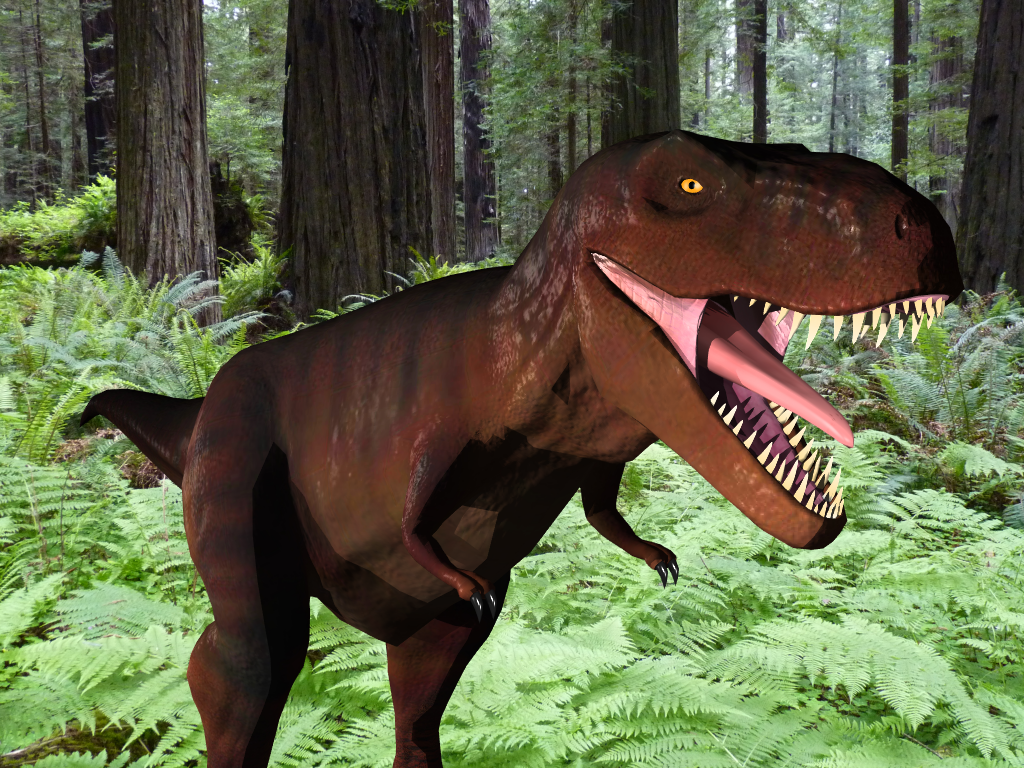
\includegraphics[scale=0.33]{./titelbild.png}
\end{center}
      }
\subtitle{Masterprojekt WS 12/13}
\author{Benedikt Mendorf}
\date{\today}

\publishers{
    \begin{tabbing}
    Betreuer: \= Prof. Dr.-Ing. Matthias Teschner\\
              \> Computer Graphics\\
              \> Albert-Ludwigs-Universität\\
    \end{tabbing}        
}

\end{titlepage}

\maketitle
\tableofcontents
\printnomenclature




\chapter{Einleitung}

"`Raytracing"' ist ein computergestütztes Verfahren, das versucht die reale Lichtausbreitung, sowie Licht-Objekt-Interaktion möglichst korrekt zu modellieren. In der Realität senden Lichtquellen Strahlen aus, die auf Objekte
treffen, wodurch gewisse Farbanteile absorbiert und andere reflektiert werden.
Gelangen diese reflektierte Strahlen auf einen Sensor, wie das menschliche Auge, kann anhand der unterschiedlichen Spektren ein Bild wahrgenommen werden. 
Beim "`Raytracing"' geht man umgekehrt vor und sendet Strahlen vom Sensor aus in eine virtuelle Szene aus Objekten und Lichtern. Dadurch werden nur die relevanten Strahlen betrachtet, die im realen Fall vom Sensor wahrgenommen worden wären.

 Aktuelle "`Raytracer"' erzeugen bereits heute nahezu fotorealistische Bilder und werden z.B. zur Produktion von Kinofilmen oder Werbespots verwendet. Aufgrund der sehr komplexen Berechnungen eignet sich "`raytracing"' im Gegensatz zur gerasterten Computergrafik eher selten für Echtzeitanwendungen.




\section{Zielsetzung}


Ziel des Projekts ist die eigenständige Implementierung eines
"`Raytracers"'. Die dazu verwendete Programmiersprache ist C++. Sie zeichnet sich besonders durch ihre Performanz aus und ist damit hervorragend zur Bewältigung der großen Anzahl an benötigten Berechnungen geeignet.

 Diese Ausarbeitung folgt dabei chronologisch den einzelnen Entwicklungsschritten. Zu Beginn werden die wichtigsten mathematischen Grundlagen geschaffen, die hauptsächlich in  der linearen Algebra angesiedelt sind. In den folgenden Kapiteln wird dann erläutert wie Strahlen in eine Szene ausgesendet werden, die Definition einfacher Objekte aussieht und Strahl-Objekt Schnitttests funktionieren, die zur Berechnung der  Objekt-Schattierung benötigt werden. Darauf folgt die Einführung von Transformationen. Diese erlauben es die Gestalt von Objekten sowie deren Lage im Raum zu ändern. Im nächsten Schritt wird die Schattierung, d.h. die Oberflächeneigenschaften von Objekten berechnet. In diesem Zusammenhang spielen Rendergleichung, sowie Lichtquellen und Materialien eine wichtige Rolle.
 
 Zu den aufwendigeren Methoden, die der "`Raytracer"'
 im finalen Zustand beherrschen wird gehört neben der Visualisierung von transparenten Dielektrika wie etwa Glas, die Verwendung von komplexen triangulierten Objekten. Diese können eine enorme Anzahl an Schnitttests erfordern, was die Implementierung einer Beschleunigungsstruktur zur Reduzierung der Schnitttest notwendig macht.
 
 
  Als Hauptleitfaden diente das Buch "`Ray Tracing from the Ground Up"' von Kevin Suffern \cite{suffern2007ray}.





%\chapter{Lineare Algebra}
%
%Grundlegend geht es beim "`Raytracing"' darum Strahlen in eine Szene, bestehend aus Objekten, zu schicken. Trifft ein Strahl ein Objekt, so wird die Beleuchtung am Schnittpunkt des Objekts berechnet.
%Zur Darstellung von Vektoren, Punkten und Transformationsmatrizen bedient sich die Computergrafik häufig Homogener Koordinaten




%Ziel des Masterprojekts ist der eigenständige Entwurf und Implementierung eines funktionsfähigen Raytracers. Grundlegend wird es darum gehen, Algorithmen und Datenstrukturen zu implementieren, die möglichst physikalisch exakt die Strahldichten $L$ (engl. radiance) der einzelnen Bildpunkte berechnen. 
%
%Wie in Abbildung~\ref{fig_Zeitplan} zu sehen ist besteht der erste Milestone darin bis Ende Dezember einen ersten rudimentären Raytracer zu erzeugen. Der Schwerpunkt wird sein, ein Framework zu erzeugen, das erstens leicht um neue Methodiken erweiterbar ist und zweitens in der Lage ist möglichst allgemeine Szenen zu verarbeiten.\\
%
%Im zweiten Teil des Projekts wird es dann darum gehen fortgeschrittenere raytracing-Methoden zur realisieren. Dabei gibt es Bereiche die besonders vertieft werden können.
%Zum Beispiel verschiedene Materialien und die zugehörigen BRDF's Materialien erzeugen, bzw. BTDF für transparente Objekte, die aus Glas oder Eis bestehen könnten. Ein weiterer interessanter Punkt wäre die Geschwindigkeitsoptimierung durch unterschiedliche Sampling-Methoden oder durch Datenstrukturen, die den Schnitttest zwischen Strahl und Objekt beschleunigen. Gerade beim Sampling besteht ein Tradeoff zwischen der Qualität des Bildes und der benötigten Zeit zum erstellen des Bildes.
 





%%%%%%%%%%%%%%%%%%%%%%%%%%%%%%%%%%%%Abbildung%%%%%%%%%%%%%%%%%%%%%%%%%%%%%%%%%%%%%%%%%%%%%%%%%%%%%%%%%%%%
%\begin{figure}[h]
%	\centering
%  
\includegraphics[width=\textwidth]{images/Zeitplan.pdf}
%	\caption{Zeitplan}
%	\label{fig_Zeitplan}
%\end{figure}
%%%%%%%%%%%%%%%%%%%%%%%%%%%%%%%%%%%%%%%%%%%%%%%%%%%%%%%%%%%%%%%%%%%%%%%%%%%%%%%%%%%%%%%%%%%%%%%%%%%%%%%%%



\chapter{Homogene Koordinaten}\label{cha:hom_koord}

Der erste Schritt auf dem Weg zum funktionsfähigen "`Raytracer"' besteht darin Objekte im dreidimensionalen Raum darstellen zu können. In der Computergrafik haben sich dafür die homogenen Koordinaten etabliert. Wie bei den inhomogenen Koordinaten existieren auch hier Spaltenvektoren. Jedoch bestehen diese aus vier anstatt drei Komponenten. Die vierte Komponente scheint zu Beginn unnütz, da sich die Position von Punkten und Objekten ebenso mit nur drei Komponenten eindeutig beschreiben lässt. Jedoch sorgt diese zusätzliche Komponente dafür, dass sich Transformationen auf eine einheitliche Art und Weise und zwar durch Multiplikation mit einer Transformationsmatrix durchführen lassen.


\section{Vektoren, Punkte und Normalen}

Neben der Vereinheitlichung von Transformationen bietet die zusätzliche Komponente, die ab jetzt mit \( w \) bezeichnet wird, den weiteren Vorteil, dass explizit zwischen Punkten und Vektoren unterschieden werden kann.

Nimmt  \( w \) den Wert \( 0 \) an, so handelt es sich um einen Vektor. Vektoren dienen der reinen Richtungsangabe und bleiben z.B. anders als Punkte bei Translationen unverändert. Ein Punkt liegt vor, wenn \( w \) Werte ungleich \( 0 \) annimmt. Sie sind mathematisch gesehen Ortsvektoren und werden durch Translation verschoben. Punkte und Vektoren werden durch einen fett geschriebenen Kleinbuchstaben gekennzeichnet:



\begin{equation*}
\text{Punkt:} \quad \boldsymbol{p} = \begin{pmatrix}
        x \\ y \\ z \\ w \ne 0
\end{pmatrix}
\qquad
\text{Vektor} \quad \boldsymbol{v} = \begin{pmatrix}
    x \\ y \\ z \\ 0
\end{pmatrix}
\end{equation*}
Die Einträge \(x, y, z\) sind die Komponenten des Vektors oder Punktes und beziehen sich wie gewohnt auf die Koordinatenachsen eines dreidimensionalen kartesischen Koordinatensystems. Die Komponente \(w\) dient als Skalierungsfaktor. Die Länge eines Vektors \( |\boldsymbol{v}| \) und Punktes \( |\boldsymbol{p}| \) ist somit gegeben durch:
\begin{equation*}
|\boldsymbol{v}| = \sqrt{x^2+y^2+z^2} \quad \quad \quad \quad
|\boldsymbol{p}| = \sqrt{\left(\frac{x}{w} \right)^2
                         + \left(\frac{y}{w}\right)^2 
                         + \left(\frac{z}{w}\right)^2
                        }
\end{equation*}

Wenn die Komponente eines Vektors oder Punktes gemeint ist, wird diese mittels Punkt-Satzzeichen dem fett geschriebenen Kleinbuchstaben angehängt. So ist mit \( \boldsymbol{p}.x \) die x-Komponente des Punktes \( \boldsymbol{p} \) gemeint.

In homogenen Koordinaten existiert ebenfalls ein Standardskalarprodukt sowie ein Kreuzprodukt, dessen Anwendung jedoch nur auf Vektoren sinnvoll ist:

\begin{align}
   \text{Skalarprodukt: }& \boldsymbol{u} \cdot \boldsymbol{v} = \boldsymbol{u}.x \cdot \boldsymbol{v}.x +  \boldsymbol{u}.y \cdot \boldsymbol{v}.y + \boldsymbol{u}.z \cdot \boldsymbol{v}.z + \boldsymbol{u}.w \cdot \boldsymbol{v}.w = \boldsymbol{u}^\intercal \boldsymbol{v} \label{eq:skalarprodukt} \\
   \text{Kreuzprodukt: }& \boldsymbol{u} \times \boldsymbol{v} = 
   \begin{pmatrix}
   \boldsymbol{u}.y \cdot \boldsymbol{v}.z - \boldsymbol{u}.z \cdot \boldsymbol{v}.y \\
   \boldsymbol{u}.z \cdot \boldsymbol{v}.x - \boldsymbol{u}.x \cdot \boldsymbol{v}.z \\
   \boldsymbol{u}.x \cdot \boldsymbol{v}.y - \boldsymbol{u}.y \cdot \boldsymbol{v}.x \\
   0
   \end{pmatrix}
\end{align}

wobei \( \boldsymbol{u}.x, \boldsymbol{v}.x, \dots, \boldsymbol{v}.w \) die Komponenten der Vektoren \( \boldsymbol{u} \text{ und } \boldsymbol{v} \) sind und \( \boldsymbol{u}^\intercal \) der transponierte Vektor von \( \boldsymbol{u} \) ist.


Vektoren, die senkrecht auf einer Oberfläche bzw. Tangentialebene eines Objekts stehen, werden in der Computergrafik zur besseren Unterscheidung als Normalen bezeichnet. Sie werden mit dem Buchstaben \( \boldsymbol{n} \) gekennzeichnet und , anders als der Name suggeriert, nicht notwendigerweise normalisiert. Die Transformation von Normalen gestaltet sich ebenfalls anders als die von Vektoren, da Normalen nach einer Transformation weiterhin orthogonal zur Oberfläche ausgerichtet sein sollen.


\section{Matrizen}\label{sec:matrizen}

In diesem Abschnitt werden die unterschiedlichen Transformationsmatrizen lediglich definiert. In Kapitel \ref{ch:transformation} wird im Detail gezeigt, wie Transformationen durchzuführen sind.

Matrizen werden beim "`Raytracing"' hauptsächlich dazu verwendet, Objekte zu transformieren. Wegen der Verwendung von homogenen Koordinaten handelt es sich dabei um \( 4 \times 4  \)-Matrizen. Sie werden durch einen fett geschriebenen Großbuchstaben gekennzeichnet.



Um Objekte entlang eines beliebigen Vektors \( \boldsymbol{a} \) zu verschieben, verwendet man eine Translationsmatrix \( \boldsymbol{T} \),

\begin{equation}
    \boldsymbol{T}( \boldsymbol{a} ) = 
    \begin{bmatrix}
        1 & 0 & 0 & a_x \\
        0 & 1 & 0 & a_y \\
        0 & 0 & 1 & a_z \\
        0 & 0 & 0 & 1
    \end{bmatrix}
\end{equation}

wobei \( a_x, a_y, a_z \) die Komponenten des Vektors \( \boldsymbol{a} \) sind. 

Rotation um die Achsen des Koordinatensystems erreicht man durch die Rotationsmatrizen,

\begin{align*}
    \boldsymbol{R_x}(\theta) &= 
    \begin{bmatrix}
        1 & 0 & 0 & 0 \\
        0 & \cos \theta & - \sin \theta & 0 \\
        0 & \sin \theta & \cos \theta & 0 \\
        0 & 0 & 0 & 1
    \end{bmatrix}, \quad
    \boldsymbol{R_y}(\theta) = 
    \begin{bmatrix}
        \cos \theta & 0 & \sin \theta & 0 \\
        0 & 1 & 0 & 0 \\
        - \sin \theta & 0 & \cos \theta & 0 \\
        0 & 0 & 0 & 1
    \end{bmatrix}, \\
    \boldsymbol{R_z}(\theta) &= 
    \begin{bmatrix}
        \cos \theta & - \sin \theta & 0 & 0 \\
        \sin \theta & \cos \theta & 0 & 0 \\
        0 & 0 & 1 & 0 \\
        0 & 0 & 0 & 1
    \end{bmatrix}
\end{align*}

wobei jeweils um die \( x, y \text{ und } z \) Achse um den Winkel \( \theta \) (im Bogenmaß) im mathematisch positiven Sinn (also gegen den Uhrzeigersinn) gedreht wird.

Soll ein Punkt an den Achsen des zugrunde liegenden Koordinatensystems gespiegelt werden, so verwendet man Reflexionsmatrizen der Form,

\begin{align*}
    \boldsymbol{S_x} = 
    \begin{bmatrix}
        -1 & 0 & 0 & 0 \\
        0 & 1 & 0 & 0 \\
        0 & 0 & 1 & 0 \\
        0 & 0 & 0 & 1 \\        
    \end{bmatrix}, \quad
    \boldsymbol{S_y} = 
    \begin{bmatrix}
        1 & 0 & 0 & 0 \\
        0 & -1 & 0 & 0 \\
        0 & 0 & 1 & 0 \\
        0 & 0 & 0 & 1
    \end{bmatrix}, \quad
    \boldsymbol{S_z} =
    \begin{bmatrix}
        1 & 0 & 0 & 0 \\
        0 & 1 & 0 & 0 \\
        0 & 0 & -1 & 0 \\
        0 & 0 & 0 & 1
    \end{bmatrix}
\end{align*}

wobei \( \boldsymbol{S_x} \) an der x-Achse und die beiden anderen Matrizen entsprechen an der y-Achse und der z-Achse spiegeln.

Um Objekte entlang der Achsen auszudehnen oder zu kontrahieren verwendet man eine Skalierungsmatrix,

\begin{equation*}
    \boldsymbol{S}(s_x, s_y, s_z) =
    \begin{bmatrix}
        s_x & 0 & 0 & 0 \\
        0 & s_y & 0 & 0 \\
        0 & 0 & s_z & 0 \\
        0 & 0 & 0 & 1
    \end{bmatrix}
\end{equation*}

wobei \( s_x, s_y \text{ und } s_z\) Faktoren sind, um die das Objekt entlang der Achsen skaliert wird.



\chapter{Strahlverfolgung}\label{ch:strahlerzeugung}

Die rudimentäre Funktionsweise eines "`Raytracers"' besteht darin, Strahlen in eine Szene, bestehend aus Objekten und Lichtquellen, auszusenden und zu überprüfen, ob diese ein Objekt treffen. Im Falle eines Schnittes wird die Schattierung des Objekts am Strahl-Objekt Schnittpunkt berechnet und diese Information wird entlang des Strahls auf eine Projektionsebene zurück propagiert. In Kapitel~\ref{ch:schattierung} wird die genaue Vorgehensweise zur Schattierungsberechnung erläutert.

In diesem Kapitel wird es darum gehen, die grundlegenden Komponenten vorzubereiten, die es dem "`Raytracer"' ermöglichen, Strahlen in eine Szene auszusenden.
Dazu benötigt man eine geeignete Repräsentation eines Strahls sowie ein Kameramodell, welches die Ansicht der Szene bestimmt. Die vom Kameramodell erzeugten Strahlen werden auch Primärstrahlen genannt. Im folgenden werden zwei Kameramodelle vorgestellt und zwar in Form einer orthografische Kamera und in Form einer Lochkamera.

Die Besonderheit besteht bei der orthografischen Kamera darin, dass die Strahlen parallel zueinander verlaufen (s. Abb~\ref{fig:orthocam}). Diese Art der Projektion wird häufig in technischen Zeichnungen verwendet, da Objekte nicht kleiner dargestellt werden, wenn sie sich von der Projektionsebenen entfernen, und somit ein besserer Vergleich der Größe von Objekten gegeben ist.

Die Lochkamera sorgt für eine perspektivische Projektion der Objekte auf die Projektionsebene. Dadurch erscheinen Objekte kleiner je weiter sie vom Beobachter entfernt sind (s. Abb~\ref{fig:pers_proj}).



\begin{minipage}[t]{0.43\textwidth}
    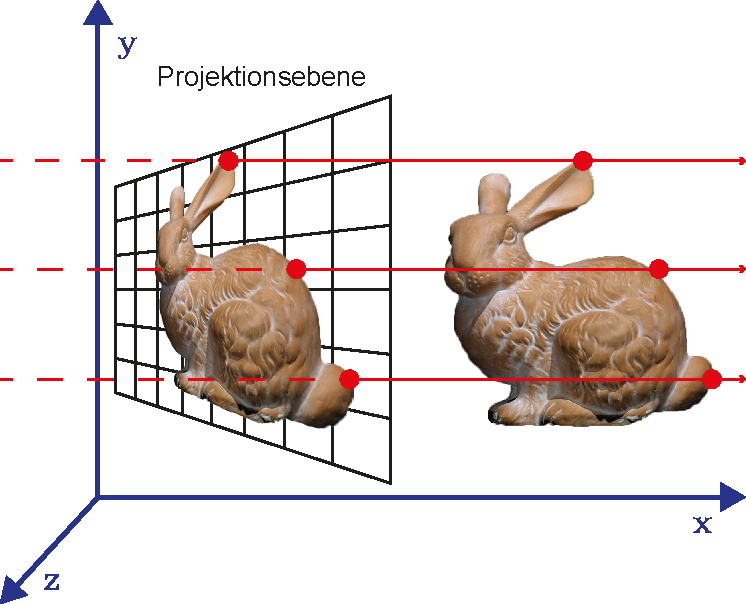
\includegraphics[width=\textwidth]{./img/strahlverfolgung/orth_proj.pdf}
    \captionof{figure}{Orthografische Kamera}
    \label{fig:orthocam}
\end{minipage}
\begin{minipage}[t]{0.51\textwidth}
    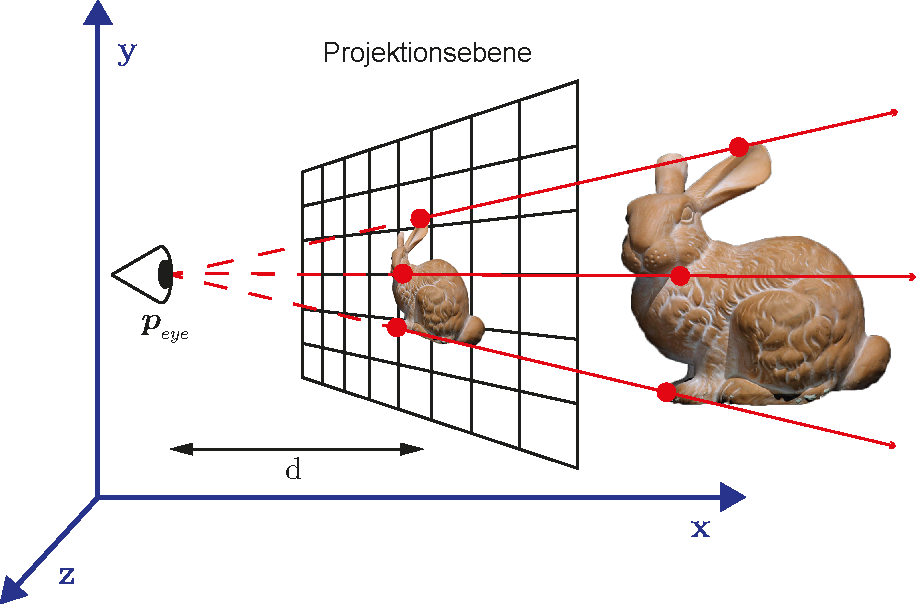
\includegraphics[width=\textwidth]{./img/strahlverfolgung/pers_proj.pdf}
    \captionof{figure}{Lochkamera}
    \label{fig:pers_proj}
\end{minipage}




\section{Strahlgleichung}

Ein Strahl besitzt die folgende parametrisierte Form:
\begin{equation}
\label{eq:Strahlgleichung}
\boldsymbol{r} = \boldsymbol{o} + t \cdot \boldsymbol{d}
\end{equation}

Der Punkt $\boldsymbol{o}$ ist der Ursprung des Strahls. Die Strahlrichtung ist durch den Vektor \( \boldsymbol{d} \) gegeben.
Der Parameter \( t \) kann beliebig gewählt werden und wird später dazu verwendet den Schnittpunkt $\boldsymbol{r}$ eines Strahls mit einem Objekt zu berechnen.

Um nun einen Strahl in eine Szene auszusenden, genügt es, seinen Ursprung \( \boldsymbol{o} \) sowie  Richtung \( \boldsymbol{d} \) festzulegen. Dies ist die Aufgabe des 
Kameramodells.


\section{Projektionsebene}

\begin{wrapfigure}[18]{r}{0.45\textwidth}    
    \vspace{-15pt}
    \centering
    
\includegraphics[width=0.44\textwidth]{./img/strahlverfolgung/projektionsebene}
    \vspace{-10pt}
    \caption{Die Projektionsebene mit Höhe $ h $, Breite $b$, Mittelpunkt $\boldsymbol{p}_{proj}$, "`Up-Vektor"' $\boldsymbol{u}_{proj}$ und Normale $\boldsymbol{n}_{proj}$. Sie ist unterteilt in gleichgroße Quadrate (PEE) mit Kantenlänge $l_{PEE}$.}
    \label{fig:projektionsebene}   
\end{wrapfigure}

Die Projektionsebene ist ein essentieller Bestandteil der nachfolgenden Kameramodelle. Tatsächlich handelt sich dabei nicht um eine Ebene, sondern um eine rechteckige Fläche mit der Höhe \( h \) und der Breite \( b \). Sie ist in kleinere Projektionsebenen-Elemente (PEE\abk{PEE}{Projektionsebenen-Elemente}) unterteilt, die nichts weiter als Quadrate   gleicher Größe sind. PEE besitzen die Kantenlänge \( l_{PEE} \). Es erweist sich als praktisch, die Größe bzw. das Seitenverhältnis der Projektionsebene festzulegen und anschließend anhand der Kantenlänge der PEE Einfluss auf die Auflösung des fertigen Bildes zu nehmen.
Denn zum Ende der Bildsynthese enthalten die PEE Farbwerte, die auf Bildelemente eines Ausgabemediums übertragen werden können. Im Falle des Monitors besteht eine einfache Abbildung darin, den Farbwert eines PEE durch genau einen Bildpunkt des Monitors ausgeben zu lassen.



\section{Orthografische Kamera}

Das Prinzip der orthografischen Kamera ist recht simpel, daher eignet sie sich ausgezeichnet, um die korrekte Funktionsweise des "`Raytracers"' zu Beginn der Implementationsphase zu überprüfen.

Sie besteht aus einer Projektionsebene (s. Abb. \ref{fig:projektionsebene} ), die innerhalb des globalen Koordinatensystems eine Position \( \boldsymbol{p}_{proj} \) und eine Ausrichtung besitzt, die durch die Normale \( \boldsymbol{n}_{proj} \) und einem "`Up-Vektor"' \( \boldsymbol{u}_{proj} \) gegeben ist. Das Ziel besteht nun darin, Strahlen durch die einzelnen PEE hindurch in die Szene zu schicken. Trifft ein Strahl auf ein Objekt, wird am Schnittpunkt die Schattierung berechnet und diese Information dem PEE zugeordnet, welches vom entsprechenden Strahl durchdrungen wurde. 

Zur Erzeugung der Strahlen empfiehlt es sich die Projektionsebene zu Beginn so zu positionieren, dass sich ihr Mittelpunkt im Ursprung des globalen Koordinatensystems befindet. 
Ihre Normale zeigt in die der z-Achse entgegengesetzte Richtung und der "`Up-Vektor"' verläuft parallel zur y-Achse. Man kann nun relativ leicht den Mittelpunkt der einzelnen PEE berechnen. Dieser dient jeweils als Strahlursprung. Die Richtung der Strahlen verläuft parallel zur z-Achse und zwar in negativer Richtung.
Die Position und Richtung der so erzeugten Strahlen werden mit \( \boldsymbol{o'} \) und \( \boldsymbol{d'} \) bezeichnet.

Diese Strahlen müssen nun vom globalen ins Kamera lokale Koordinatensystem transformiert werden. Dies gelingt, indem man eine Orthonormalbasis (ONB\abk{ONB}{Orthonormalbasis}) aus \( \boldsymbol{n}_{proj} \) und \( \boldsymbol{u}_{proj} \) erzeugt, dann einen Basiswechsel durchführt und anschließend um den Vektor \( \boldsymbol{v} = \boldsymbol{p}_{proj} - \begin{pmatrix} 0 & 0 & 0 & 1 \end{pmatrix}^\intercal \) verschiebt.

Es sei vorausgesetzt, dass:

\begin{equation*}
|\boldsymbol{n}_{proj}| = 1; \qquad |\boldsymbol{u}_{proj}| = 1; \qquad \boldsymbol{n}_{proj} \cdot \boldsymbol{u}_{proj} = 0 
\end{equation*}

dann ist die ONB gegeben durch:

\begin{equation}
    \boldsymbol{e}_1 = \boldsymbol{n}_{proj} \times \boldsymbol{u}_{proj}; \qquad \boldsymbol{e}_2 = \boldsymbol{u}_{proj}; \qquad \boldsymbol{e}_3 = -\boldsymbol{n}_{proj}
    \label{eq:onb}
\end{equation}

Basiswechsel durchführen mit:

\begin{align}
    \boldsymbol{o''} &= \boldsymbol{o'}.x \cdot \boldsymbol{e}_1 + \boldsymbol{o'}.{y} \cdot \boldsymbol{e}_2 + \boldsymbol{o'}.{z} \cdot \boldsymbol{e}_3 + 
                      \boldsymbol{o'}.{w} \cdot \begin{pmatrix} 0 & 0 & 0 & 1 \end{pmatrix}^\intercal \\
    \boldsymbol{d}         &= \boldsymbol{d'}.{x} \cdot \boldsymbol{e}_1 + \boldsymbol{d'}.{y} \cdot \boldsymbol{e}_2 + \boldsymbol{d'}.{z} \cdot \boldsymbol{e}_3 \label{eq:onb_richtung}
\end{align}

wobei \( \boldsymbol{o'}.{x}, \boldsymbol{d'}.{x}, \dots, \boldsymbol{d'}.w\) usw. die jeweilige Komponente von \( \boldsymbol{o'} \) und \( \boldsymbol{d}' \) bezeichnet.
Anschließend um den Vektor \( \boldsymbol{v} \) verschieben.

\begin{equation*}
    \boldsymbol{o} = \boldsymbol{o''} + \boldsymbol{v}
\end{equation*}

Im Fall der orthografischen Kamera kann Gleichung~\ref{eq:onb_richtung} entfallen, da aufgrund des senkrechten Austrittswinkel der Strahlen aus der Projektionsebene einfach \( \boldsymbol{d} = \boldsymbol{n}_{proj} \) gesetzt werden kann.


\section{Lochkamera}

Bei realen Lochkameras werden Objekte an der Lochblende um \( 180^\circ \) gedreht auf einen Film oder Sensor abgebildet. Dieser Umstand lässt sich beim virtuellen Kameramodell gut vermeiden, indem man den Betrachter an die Position der Lochblende setzt und ihn auf die Szene richtet. Die Projektionsebene nimmt die Rolle des Films ein und wird zwischen Betrachter und Szene eingebracht. Je kleiner das Loch ist, desto schärfer wird das Bild in der Realität, da störende Randstrahlen abgeschirmt werden.

Die Position des Betrachters \( \boldsymbol{p}_{eye} \) dient als Startpunkt für die Strahlen und kann als unendlich kleines Loch angesehen werden, wodurch maximal scharfe Bilder erzeugt werden. Bei der orthografischen Kamera spielt es generell keine Rolle, ob der Startpunkt der Strahlen auf der Projektionsebenen liegt oder irgendwo davor. Bei der Lochkamera verhält es sich komplett anders. Die Entfernung des Betrachters, in Abb.~\ref{fig:pers_proj} mit \( d \) gekennzeichnet, entscheidet nämlich darüber, wie groß das Sichtfeld ausfällt. Durch folgende Formel lässt sich \( d \) bestimmen:

\begin{equation*}   
     d = \frac{b}{2 \cdot \tan{(\phi_{hfov} \cdot \frac{1}{2})}}
\end{equation*}

\( b \) ist die Breite der Projektionsebene.
\( \phi_{hfov} \) ist der Winkel, der zwischen \( \boldsymbol{p}_{eye} \) und Mittelpunkt der Projektionsebene, sowie \( \boldsymbol{p}_{eye} \) und Mittelpunkt der seitlichen Kante der Projektionsebene aufgespannt wird. Das Sichtfeld des Menschen beträgt fast \( 180^\circ \), was im Bogenmaß einem \( \phi_{hfov} \) von \( \pi \) entsprechen würde. Da der Monitor jedoch nur einen Teil des menschlichen Sichtfelds einnimmt, hat sich ein Wert von \( \frac{\pi}{2} \) für \( \phi_{hfov} \) als geeignet herausgestellt.

Um Strahlen zu erzeugen, richtet man die Projektionsebene wie bei der orthografischen Kamera gezeigt aus, d.h. im Mittelpunkt des globalen Koordinatensystems und die Normale in Richtung negativer z-Achse. Der Betrachter  wird an Position \( \boldsymbol{p}_{eye} \) = \( \begin{pmatrix} 0 & 0 & d & 1 \end{pmatrix}^\intercal \) gesetzt. Sei \( \boldsymbol{m}_{PEE} \) der Mittelpunkt eines PEE, dann ergibt sich die vorläufige Richtung \( \boldsymbol{d'} \) eines Strahls aus \( \boldsymbol{d'} = \boldsymbol{m}_{PEE} - \boldsymbol{p}_{eye} \). Anschließend erzeugt man eine ONB nach Gleichung~\ref{eq:onb} und berechnet die endgültige Strahlrichtung \( \boldsymbol{d} \), wie in \ref{eq:onb_richtung} gezeigt. Für den Strahlursprung lässt sich einfach \( \boldsymbol{o} = \boldsymbol{p}_{eye}\) setzen.




\chapter{Objekte und Schnitttests}\label{ch:obj_schnitt}

Bis jetzt ist der "`Raytracer"' in der Lage Strahlen gemäß eines gewünschten Kameramodells in die Szene zu schicken. Der nächste Schritt besteht nun darin, die Szene mit Objekten zu bevölkern. Anschließend muss überprüft werden, ob ein ausgesandter Strahl eines der Objekte trifft. Im Falle, dass mehrere Objekte hintereinander liegen und es somit zu mehreren Schnitten kommt, wird immer der Schnittpunkt gesucht, der dem Betrachter am nächsten ist. Abb.~\ref{fig:schnitt_objekte} zeigt einen solchen Fall. Die Durchdringung der Objekte, wird durch Verwendung des zum Betrachter nächsten Schnittpunkts korrekt dargestellt.

Neben dem nächstgelegenen Schnittpunkt wird auch noch eine Normale benötigt, um die Schattierung des Objekts berechnen zu können.
Das folgende Kapitel zeigt die Definition verschiedener Objekte und demonstriert den Ablauf der jeweiligen Schnitttests. Zudem wird für gefundene Schnittpunkte eine Normale erzeugt, die zur Schattierungsberechnung benötig wird.

\begin{figure}[ht]
    \centering
    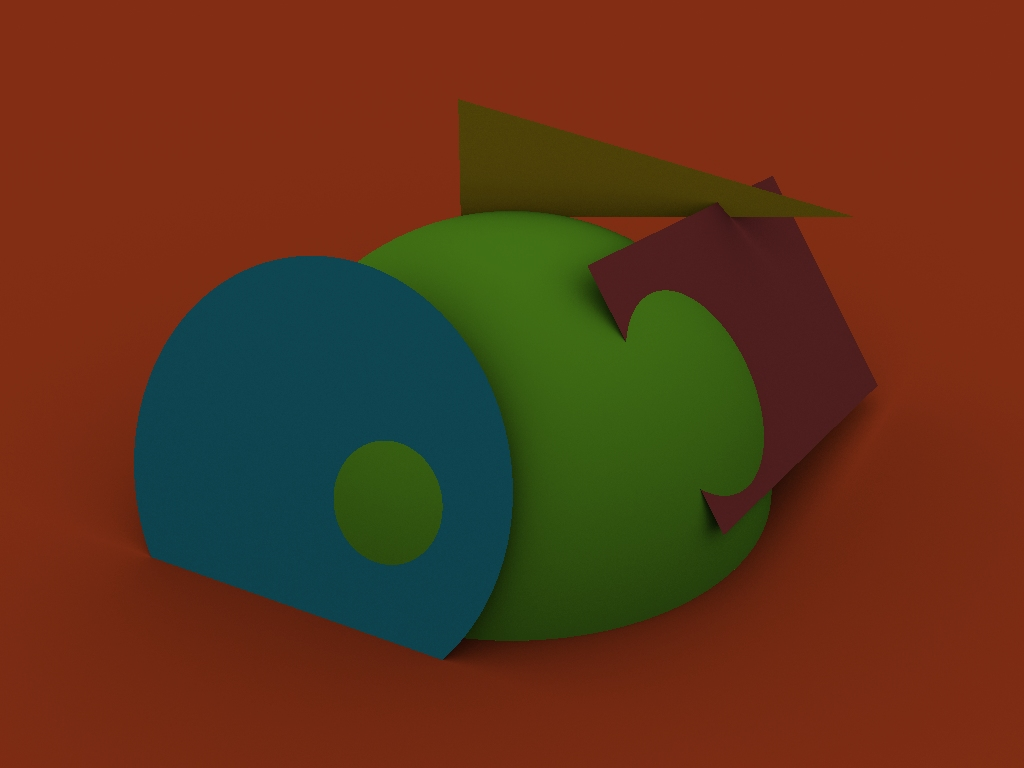
\includegraphics[width=0.8\textwidth]{./img/obj_schnitt/schnitt_objekte.jpg}
    \caption{Schnitt einer Kugel mit Ebene, Scheibe, Rechteck und Dreieck. Der zum Betrachter nächste Schnittpunkt wird zu korrekten Darstellung der Objektdurchdringungen benötigt.}
    \label{fig:schnitt_objekte}
\end{figure}


\section{Ebene}
Der Schnitttest mit einer Ebene gestaltet sich sehr einfach und dient als Grundlage für weitere Schnitttests mit Objekten wie Rechtecken, Dreiecken oder Scheiben. Dazu betrachtet man folgende implizite Form der Ebene:
\begin{equation}
(\boldsymbol{p} - \boldsymbol{a}) \cdot \boldsymbol{n} = 0
\end{equation}
wobei $\boldsymbol{a}$ ein Ortsvektor in der Ebene ist und $\boldsymbol{n}$  eine Normale, die somit senkrecht auf der Ebene steht.
Den impliziten Charakter erhält die Gleichung dadurch, dass sie eine Bedingung an Punkte $\boldsymbol{p}$ in der Ebene stellt. Ein Punkt liegt nämlich genau dann in der Ebene, wenn die Normale $\boldsymbol{n}$ senkrecht auf dem Vektor von $\boldsymbol{a}$ nach $\boldsymbol{p}$ steht und das Skalarprodukt somit gleich Null ist.

Das Ziel ist es jetzt, die Strahlgleichung~\ref{eq:Strahlgleichung} einzusetzen und den Parameter $t$ zu bestimmen, wobei nur für positive \(t\) tatsächlich ein Schnitt vorliegt.


\begin{align}
 0 &= (\boldsymbol{o} + t \cdot \boldsymbol{d} - \boldsymbol{a}) \cdot \boldsymbol{n} 		\nonumber\\
\text{Finale Form:} \qquad t &= \frac{(\boldsymbol{a} - \boldsymbol{o}) \cdot \boldsymbol{n} }{\boldsymbol{d} \cdot \boldsymbol{n} } \label{eq:ebenenschnitt}
\end{align}

Zum Schattieren der Ebene wird die Normale \( \boldsymbol{n} \) verwendet, die bereits zur Definition der Ebene diente. Der Schnittpunkt \( \boldsymbol{r} \) lässt sich nun leicht durch Einsetzen von \( t \) in die Strahlgleichung~\ref{eq:Strahlgleichung} bestimmen, da Strahlursprung \( \boldsymbol{o} \) und Strahlrichtung \( \boldsymbol{d} \) durch das Kameramodell bereits festgelegt sind.


\section{Rechteck}

\FloatBarrier

%\begin{figure}
%    \centering
%    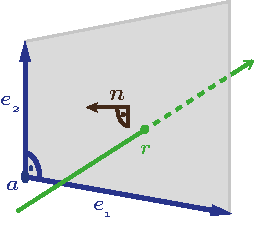
\includegraphics[scale=1.5]{img/obj_schnitt/rechteck.pdf}
%    \caption{Definition Rechteck  }
%    \label{fig:rechteck}
%\end{figure}


\begin{wrapfigure}[18]{r}{0.45\textwidth}    
    \vspace{-15pt}
    \centering
    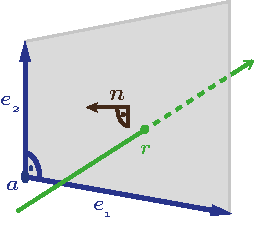
\includegraphics[width=0.44\textwidth]{img/obj_schnitt/rechteck.pdf}
    \vspace{-10pt}
    \caption{Definition eines Rechtecks durch linken unteren Stützpunkt $\boldsymbol{a}$, Kantenvektoren $\boldsymbol{e_1}, \boldsymbol{e_2}$ und Normale $\boldsymbol{n}$. Ein Strahl schneidet das Rechteck am Schnittpunkt $\boldsymbol{r}$.  }
    \label{fig:rechteck}
\end{wrapfigure}


Eine einfache Repräsentation eines Rechtecks besteht darin, den linken unteren Punkt \(\boldsymbol{a}\) anzugeben und die Ausdehnung des Rechtecks durch zwei orthogonal verlaufende Vektoren \(\boldsymbol{e_1}\) und \(\boldsymbol{e_2}\) festzulegen (siehe Abbildung~\ref{fig:rechteck}). Diese Informationen sind bereits ausreichend, um die auf dem Rechteck senkrecht stehende Normale \(\boldsymbol{n}\) durch den Term \( \left( \boldsymbol{e_1} \times \boldsymbol{e_2} \right) \cdot \left( |\boldsymbol{e_1} \times \boldsymbol{e_2}| \right)^{-1} \) zu bestimmen. Dennoch ist es in der Implementation sinnvoll, die explizite Angabe der Normalen zu erlauben, da auf diese Weise festgelegt werden kann, für welche Seite die Schattierungsberechnungen durchgeführt werden soll.


Der eigentliche Schnitttest verläuft nun in zwei Schritten. Zuerst wird ein Ebenen-Schnitttest nach Gleichung~\ref{eq:ebenenschnitt} durchgeführt, wodurch man den Parameter \(t\) erhält. Durch die Strahlgleichung~\ref{eq:Strahlgleichung} lässt sich nun, falls existent, exakt der Schnittpunkt \(\boldsymbol{r}\) berechnen.

Im nächsten Schritt erzeugt man einen Vektor \(\boldsymbol{v}  = \boldsymbol{r} - \boldsymbol{a}\). Diesen projiziert man auf Basisvektoren, die die gleiche Richtung wie \( \boldsymbol{e_1} \) und \( \boldsymbol{e_2} \) besitzen.
Damit erhält man die Länge des Vektors \( \boldsymbol{v} \) in Richtung von \( \boldsymbol{e_1} \) und \( \boldsymbol{e_2} \). Die so projizierten Vektoren \( \boldsymbol{v_{e_1} } \) und \( \boldsymbol{v_{e_2} } \) erhält man daher durch:
\begin{align*}
    \boldsymbol{v_{e_1} } = \frac{ \boldsymbol{v} \cdot \boldsymbol{e_1} }{ |\boldsymbol{e_1}| }  \qquad \qquad \qquad
    \boldsymbol{v_{e_2} } = \frac{ \boldsymbol{v} \cdot \boldsymbol{e_2} }{ |\boldsymbol{e_2}| }
\end{align*}


Der Punkt \( \boldsymbol{r} \) ist genau dann ein Schnittpunkt des Rechtecks, wenn die Längen von \( \boldsymbol{v_{e_1} } \) und \( \boldsymbol{v_{e_2} } \) positiv sind und nicht länger als ihre jeweiligen Projektionsachsen. Daher müssen folgende Ungleichungen gelten:
\begin{align*}
    0 \leq |\boldsymbol{v_{e_1}}| \leq |\boldsymbol{e_1}| \qquad \text{und} \qquad
    0 \leq |\boldsymbol{v_{e_2}}| \leq |\boldsymbol{e_2}|
\end{align*}

Momentan muss noch eine Quadratwurzel berechnet werden, um \( |\boldsymbol{v_{e_1}}| \) zu erhalten. Diese Operation ist jedoch relativ teuer und lässt sich einfach vermeiden, indem man die Ungleichung umformt:
\begin{align}
  \text{Final:} \qquad  0 \leq \boldsymbol{v} \cdot \boldsymbol{e_1}  \leq \boldsymbol{e_1} \qquad \text{und} \qquad
    0 \leq \boldsymbol{v} \cdot \boldsymbol{e_2}  \leq \boldsymbol{e_2}
\end{align}

\FloatBarrier

\section{Scheibe}

Eine Scheibe wird durch drei Komponenten definiert. Dem Mittelpunkt \( \boldsymbol{a} \), einer Normalen \( \boldsymbol{n} \), die senkrecht auf der Scheibe steht und somit deren Lage festlegt, und dem Radius \( r \).
Zuerst wird auch hier ein Ebenen-Schnitttest nach Gleichung \ref{eq:ebenenschnitt} durchgeführt.
Anschließend wird geprüft, ob der Schnittpunkt \( \boldsymbol{r} \) (berechnet durch Gleichung \ref{eq:Strahlgleichung}) in der Scheibe liegt. Der Ebenenschnittpunkt \( \boldsymbol{r} \) liegt in der Scheibe, wenn folgende Ungleichung erfüllt ist:
\begin{equation}
    0 \leq |\boldsymbol{r} - \boldsymbol{a}|^2 \leq r^2
\end{equation}



\section{Dreieck}\label{sec:dreieck}

Der nun folgende Schnitttest wird im Buch "`Physically Based Rendering"' \cite{pharrhumphrey2010Physically} beschrieben und geht zurück auf die Arbeit von Thomas Möller und Ben Trumbore \cite{moller1997FasMinStoRayInt}. Wie bei den bisher vorgestellten Schnitttests könnte man zuerst den Schnittpunkt mit der durch das Dreieck aufgespannten Ebenen berechnen und anschließend durch einen Halbseitentest feststellen, ob dieser Schnittpunkt innerhalb des Dreiecks liegt. Die Methode von \cite{moller1997FasMinStoRayInt} löst dieses Problem allerdings eleganter durch die Verwendung von baryzentrischen Koordinaten, die auf die Arbeit von August Ferdinand Möbius~\cite{mobius1827DerBarCal} zurückgehen. Man erhält dadurch nicht nur die Position des Schnittpunktes im globalen Koordinatensystems, sondern auch dessen Lage innerhalb des Dreiecks, ausgedrückt durch baryzentrische Koordinaten. Letzterer Aspekt wird noch eine wichtige Rolle beim Texturieren von Objekten in Kapitel~\ref{ch:texturierung} spielen. Zudem wird in \cite{moller1997FasMinStoRayInt} gezeigt, dass sich der Speicherverbrauch durch das Vermeiden des Strahl-Ebenen Schnitts verringern lässt.

%\begin{figure}
%    \centering
%    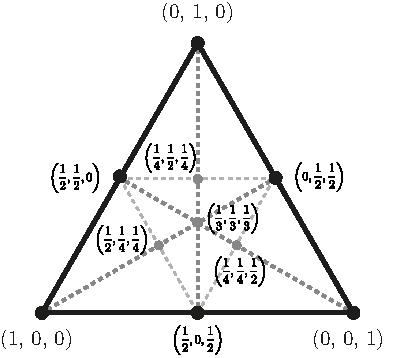
\includegraphics[scale=1]{img/obj_schnitt/baryzentrum.pdf}
%    \caption{Baryzentrische Koordinaten im Dreieck.}
%    \label{fig:baryzentrum}
%\end{figure}


\begin{wrapfigure}[20]{r}{0.45\textwidth}    
    \vspace{-15pt}
    \centering
    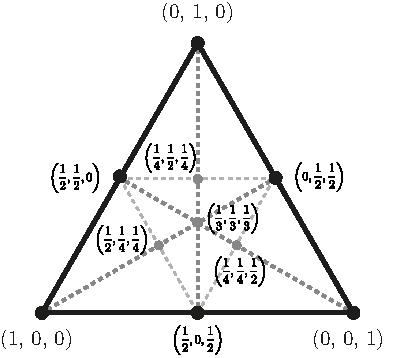
\includegraphics[width=0.44\textwidth]{img/obj_schnitt/baryzentrum.pdf}
    \vspace{-10pt}
    \caption{Baryzentrische Koordinaten im Dreieck. Alle Punkte im Dreieck können als gewichtete Summe der 3 Eckpunkten dargestellt werde.}
    \label{fig:baryzentrum}
\end{wrapfigure} 
 

Ein Dreieck ist gegeben durch drei Punkte \( \boldsymbol{p_0}, \boldsymbol{p_1} \) und \( \boldsymbol{p_2} \). Die Normale \( \boldsymbol{n} \) lässt sich aus dem Kreuzprodukt \( \boldsymbol{n} = (\boldsymbol{p_1} - \boldsymbol{p_0}) \times (\boldsymbol{p_2} - \boldsymbol{p_0})  \) errechnen. Das Ziel ist es nun, einen Schnitt festzustellen und den Schnittpunkt \( \boldsymbol{r} \) durch baryzentrische Koordinaten auszudrücken. Dazu werden die Koeffizienten \( \alpha, \beta \text{ und } \gamma \) eingeführt, die als Gewichte für die Punkte \( \boldsymbol{p_0}, \boldsymbol{p_1} \) und \( \boldsymbol{p_2} \) dienen. Sie besitzen daher die gleiche Bedeutung wie die Massen bei der Bestimmung des Massenschwerpunkts. Der gesuchte Schnittpunkt \( \boldsymbol{r} \) lässt sich somit als gewichtetes Mittel der Dreieckspunkte darstellen:

\begin{equation}
\label{eq:bary}
    \boldsymbol{r} = \alpha \cdot \boldsymbol{p_0} + \beta \cdot \boldsymbol{p_1} + \gamma \cdot \boldsymbol{p_2}
\end{equation}

Da nur Schnittpunkte gesucht sind, die innerhalb des Dreiecks liegen, müssen die Gewichte stets positiv sein. Außerdem gilt für jeden Punkt innerhalb des Dreiecks, dass sich die Gewichte zu \( 1 \) summieren. Es gelten somit die folgenden Bedingungen:

\begin{align}
\label{eq:bary_bedingung1}
\text{Bedingung 1:} &      \qquad 0 \leq \alpha \leq 1;  \qquad 0 \leq \beta \leq 1; \qquad 0 \le \gamma \leq 1 \\
\label{eq:bary_bedingung2}
\text{Bedingung 2:} &      \qquad \alpha + \beta + \gamma = 1 
\end{align}


Die zweite Bedingung \ref{eq:bary_bedingung2} ermöglicht es \( \alpha \) durch \( \beta \) und \( \gamma \) auszudrücken. Nach Einsetzen der Strahlgleichung \ref{eq:Strahlgleichung} für \( \boldsymbol{r} \) ergibt sich folgende Form: 


\begin{equation*}
    \boldsymbol{o} + t \cdot \boldsymbol{d} = (1 - \beta - \gamma) \cdot \boldsymbol{p_0} + \beta \cdot \boldsymbol{p_1} + \gamma \cdot \boldsymbol{p_2}
\end{equation*}

Der nächste Schritt besteht darin, diese Gleichung in eine Form zu bringen, die mit Hilfe der Cramerschen Regel lösbar ist. Sie hat die Form \( \boldsymbol{A} \cdot \boldsymbol{x} = \boldsymbol{b} \), wobei eine Lösung für \( \boldsymbol{x} \) gesucht ist. Nach dem Umformen erhält man:

\begin{equation*}
% Matrix-vector equation with annotated braces
\underbrace{%
    \begin{bmatrix}
        \boldsymbol{d} & \boldsymbol{p_1}-\boldsymbol{p_0} & \boldsymbol{p_2}-\boldsymbol{p_0}
    \end{bmatrix}%
}_{\boldsymbol{A}}
\cdot
\underbrace{%
    \begin{pmatrix} t \\ \beta \\ \gamma \end{pmatrix}%
}_{\boldsymbol{x}}
\;=\;
\underbrace{%
    \boldsymbol{o}-\boldsymbol{p_0}%
}_{\boldsymbol{b}}
\end{equation*}

Abkürzend wird hier nur die resultierende Gleichung zitiert. Die vollständige Herleitung kann in \cite{pharrhumphrey2010Physically} (S. 140 ff) nachgelesen werden.
Mit folgenden Substitutionen

\begin{align*}
    \boldsymbol{e_1} &= \boldsymbol{p_1} - \boldsymbol{p_0};  & \boldsymbol{e_2} &= \boldsymbol{p_2} - \boldsymbol{p_0}; & \boldsymbol{s} = \boldsymbol{o} - \boldsymbol{p_0};\\
    \boldsymbol{s_1} &= \boldsymbol{d} \times \boldsymbol{e_2};   &  \boldsymbol{s_2} &= \boldsymbol{s} \times \boldsymbol{e_1}; &
\end{align*}

sind nun alle Komponenten bekannt, um die finale Gleichung \ref{eq:triangle_final} zu lösen.

\begin{equation}
    \label{eq:triangle_final}
    \text{Finale Form:} \qquad \begin{pmatrix} t \\ \beta \\ \gamma \end{pmatrix} = \frac{1}{\boldsymbol{s_1} \cdot \boldsymbol{e_1} } \cdot
    \begin{pmatrix}
        \boldsymbol{s_2} \cdot \boldsymbol{e_2} \\ \boldsymbol{s_1} \cdot \boldsymbol{s} \\ \boldsymbol{s_2} \cdot \boldsymbol{d}
    \end{pmatrix} 
\end{equation}

Abschließend ist zu bemerken, dass die Berechnung der Gleichung \ref{eq:triangle_final} unter Umständen frühzeitig beendet werden kann, falls kein Schnitt vorliegt. Dazu
verwendet man Bedingung \ref{eq:bary_bedingung1} und \ref{eq:bary_bedingung2} sowie die Tatsache, dass eine Division durch 0 nicht definiert ist.
Algorithmus \ref{alg:dreieck_schnitt} veranschaulicht in welcher Reihenfolge deshalb die einzelnen Komponenten berechnet werden sollten und welche Bedingungen verletzt sein müssen, damit die Berechnungen frühzeitig mit dem Rückgabewert "`false"' beendet werden.

\begin{algorithm}[H]
    \caption{Dreieck Schnitttest}
    \label{alg:dreieck_schnitt}
    \begin{algorithmic}[1]
        \State \(divisor \gets \boldsymbol{s_1} \cdot \boldsymbol{e_1}\)
        \If{\( divisor = 0 \)}
            \State\Return{\textbf{false}}
        \EndIf
        \State \( \beta \gets \boldsymbol{s_1} \cdot \boldsymbol{s} \cdot divisor^{-1} \)
        \If{\( \beta < 0 \; \textbf{or} \; \beta > 1 \)}
            \State\Return{\textbf{false}}
        \EndIf
        \State \( \gamma \gets \boldsymbol{s_2} \cdot \boldsymbol{d} \cdot divisor^{-1} \)
        \If{\( \gamma < 0 \; \textbf{or} \; \beta + \gamma > 1 \)}
            \State\Return{\textbf{false}}
        \EndIf
        \State \( t \gets \boldsymbol{s_2} \cdot \boldsymbol{e_2} \cdot divisor^{-1} \)
        \State\Return{\textbf{true}}   
    \end{algorithmic}
\end{algorithm}


\section{Kugel}

Eine Kugel besitzt einen Mittelpunkt \( \boldsymbol{c} \) und einen Radius \( r \). An alle Punkte \( \boldsymbol{p} \) auf der Kugeloberfläche wird durch die implizite Form folgende Bedingung gestellt:

\begin{equation*}
    (\boldsymbol{p} - \boldsymbol{c}) \cdot (\boldsymbol{p} - \boldsymbol{c}) - r^2 = 0
\end{equation*}

D.h. die Entfernung eines Punktes \( \boldsymbol{p} \) vom Mittelpunkt \( \boldsymbol{c} \) muss genau dem Radius entsprechen. Nach Einsetzen der Strahlgleichung~\ref{eq:Strahlgleichung} in obige Gleichung und Umformen erhält man eine quadratische Gleichung, die z.B. durch die a-b-c-Formel gelöst werden kann:


\begin{align*}
(\boldsymbol{o} + t \boldsymbol{d} - \boldsymbol{c}) \cdot (\boldsymbol{o} + t \boldsymbol{d} - \boldsymbol{c}) - r^2 &= 0 \\
\overbrace{ \boldsymbol{d} \cdot \boldsymbol{d} }^{a} \, t^2
+ \overbrace{ 2 (\boldsymbol{o} - \boldsymbol{c}) \cdot \boldsymbol{d} }^{b} \, t
+ \overbrace{ (\boldsymbol{o} - \boldsymbol{c}) \cdot (\boldsymbol{o} - \boldsymbol{c}) - r^2 }^{c} &= 0
\end{align*}
}

Eine quadratische Gleichung hat typischerweise eine, zwei oder keine Lösung. Dies hängt davon ab, wie der Strahl die Kugel trifft und welche Werte die Diskriminante annimmt. Verfehlt der Strahl die Kugel, gibt es keine Lösung, tangiert er sie, gibt es eine Lösung und wenn er sie durchdringt, gibt es einen Ein- und Austrittspunkt und somit zwei Lösungen. Ein Strahl kann auch innerhalb einer Kugel beginnen, wobei mathematisch zwei Lösungen existieren, jedoch befindet sich der Schnittpunkt einer der Lösungen hinter dem Strahlursprung und ist unbrauchbar. Dies wird deutlich durch den Parameter \( t \), der in diesem Fall einen negativen Wert annimmt. Ähnlich ist der Fall, in dem der Strahl exakt auf der Kugel"=oberfläche beginnt. Es ist somit sinnvoll, einen gefundenen Schnittpunkt nur dann als solchen zuzulassen, wenn \( t > 0 \) gilt. 

Algorithmus~\ref{alg:kugel_schnitt} demonstriert die Vorgehensweise und gibt \textbf{true} zurück bei erfolgreichem Schnitt:

\begin{algorithm}[H]
    \caption{Kugel Schnitttest}
    \label{alg:kugel_schnitt}
    \begin{algorithmic}[1]
        \State \( diskriminante \gets b \cdot b - 4 \cdot a \cdot c  \)
        \If {\(  diskriminante < 0 \)}
        \State\Return{\textbf{false}}
        \EndIf
        \State \( t \gets -b - \sqrt{diskriminante} \cdot (2a)^{-1}  \) \Comment{Teste zuerst die kleinere Wurzel..}
        \If {\( t > 0 \)}
        \State\Return{\textbf{true}}
        \EndIf
        \State \( t \gets -b + \sqrt{diskriminante} \cdot (2a)^{-1}  \) \Comment{.. jetzt die größere Wurzel}
        \If {\( t > 0 \)}
        \State\Return{\textbf{true}}
        \EndIf
        \State\Return{\textbf{false}}     
    \end{algorithmic}
\end{algorithm}

Nun kann man wieder \( t \) in Strahlgleichung~\ref{eq:Strahlgleichung} einsetzen und Schnittpunkt \( \boldsymbol{r} \) berechnen.
Zuletzt fehlt nur noch die Normale am Schnittpunkt. Diese ergibt sich einfach aus:

\begin{equation*}
    \boldsymbol{n} = \frac{\boldsymbol{r} - \boldsymbol{c} } {|\boldsymbol{r} - \boldsymbol{c}|}
\end{equation*}


\section{Selbstschnitt}

Bei den oben beschriebenen mathematischen Herleitungen der Schnitttests bleibt ein Problem verborgen, das erst in der Implementation erkennbar wird. Dabei handelt es sich um den Selbstschnitt. Ein Strahl wird von der Oberfläche eines Objekts ausgesandt und der Schnitttest erkennt fälschlicherweise einen Schnitt mit eben diesem Objekt. Aufgrund von Ungenauigkeiten bei der Berechnung und Darstellung von Fließkommazahlen liefert der Test \( t > 0 \) oft noch falsche Schnitte, weshalb es sich bewährt hat, gegen einen sehr kleinen Wert \( k_\epsilon \) zu testen, also \( t > k_\epsilon \), wobei sich ein Wert von \( 10^{-4} \) für \( k_\epsilon \) bewährt hat.




\chapter{Transformation} \label{ch:transformation}


In Abschnitt~\ref{sec:matrizen} wurden bereits Transformationsmatrizen eingeführt, die vorab verschiedene Transformationsarten vorstellten.
In diesem Kapitel wird es darum gehen, zu zeigen, wie die Transformation für Objekte genau durchzuführen ist.
Anders als bei der gerasterten 3D-Computergrafik bestehen Objekte beim "`Raytracing"' nicht notwendigerweise aus einer Menge von Polygonen, deren Punkte sich relativ einfach transformieren lassen.
So existieren z.B. Objekte mit komplexeren impliziten Darstellungsformen als die bereits vorgestellten. Für diese Objekte erscheint eine direkte Transformation aussichtslos. Der Trick wird deshalb darin bestehen, nicht direkt die Objekte, sondern den Strahl auf eine geeignete Art und Weise zu transformieren, um so zum selben Ergebnis zu kommen.

\section{Grundlagen }

Die Transformation von Punkten oder Vektoren funktioniert über das Matrix-Vektor-Produkt:

\begin{equation*}
    \boldsymbol{p'} = \boldsymbol{T} \cdot \boldsymbol{p}
\end{equation*}

mit \( \boldsymbol{T} \in \mathds{R}^{4 \times 4} \) und \( \boldsymbol{p} \in \mathds{R}^4 \). Punkt \( \boldsymbol{p'} \) geht aus der Transformation von \( \boldsymbol{p} \) mit Transformationsmatrix \( \boldsymbol{T} \) hervor.

Transformationen lassen sich durch linksseitige Multiplikation mit der inversen Transformationsmatrix \( \boldsymbol{T}^{-1} \) umkehren:

\begin{align*}
    \boldsymbol{T}^{-1} \cdot \boldsymbol{T} \cdot \boldsymbol{p} &= \boldsymbol{T}^{-1} \cdot \boldsymbol{p'}\\
    \mathds{1} \cdot \boldsymbol{p} &= \boldsymbol{T}^{-1} \cdot \boldsymbol{p'}\\
    \boldsymbol{p} &= \boldsymbol{T}^{-1} \cdot \boldsymbol{p'}
\end{align*}

wobei \( \mathds{1} \) die \( 4 \times 4 \) Einheitsmatrix ist.

Für die in Abschnitt~\ref{sec:matrizen} vorgestellten Matrizen sehen die inversen Transformationsmatrizen wie folgt aus:

\begin{align*}
    &\text{Translsationsmatrix: } &  &\boldsymbol{T}^{-1}(\boldsymbol{a}) = \boldsymbol{T}(-\boldsymbol{a})\\
    &\text{Rotationsmatrix: }    &  &\boldsymbol{R_x}^{-1}(\theta) = \boldsymbol{R_x}(-\theta) = \boldsymbol{R_x}^{\intercal}(\theta); &  &\boldsymbol{R_y}(\theta) \text{ und }  \boldsymbol{R_z}(\theta) \text{ analog}\\
    &\text{Reflexionsmatrix: }   &  &\boldsymbol{S_x}^{-1} = \boldsymbol{S_x}; &  &\boldsymbol{S_y} \text{ und } \boldsymbol{S_z} \text{ analog}\\
    &\text{Skalierungsmatrix: }  &  &\boldsymbol{S}^{-1}(s_x, s_y, s_z) = \boldsymbol{S}(s_x^{-1}, s_y^{-1}, s_z^{-1})
\end{align*}

Bei der Rotationsmatrix fällt auf, dass ihre Transponierte auch gleichzeitig ihre Inverse ist. Diese Eigenschaft gilt für alle orthogonalen Matrizen, wozu auch die Rotationsmatrix gehört.

Wenn auf demselben Vektor oder Punkt nacheinander mehrere Transformationen durchgeführt werden, spricht man von einer verketteten Transformation: 

\begin{equation*}
\boldsymbol{T_C} = \boldsymbol{T_n} \cdots \boldsymbol{T_2} \cdot \boldsymbol{T_1}
\end{equation*}


\( \boldsymbol{T_1} \) ist dabei die erste anzuwendende Transformation und  \( \boldsymbol{T_n} \) die letzte. Durch Multiplikation der einzelnen Transformationsmatrizen
entsteht eine Ergebnismatrix \( \boldsymbol{T_C} \). Mit Hilfe von \( \boldsymbol{T_C} \) kann dann durch eine einzige Matrix-Vektor-Multiplikation die komplette Sequenz an Transformationen auf einen Punkt oder Vektor angewandt werden. 
Ein Problem ist, dass \( \boldsymbol{T_C} \) zu einer Matrix mit allgemeiner Form degenerieren kann, was das Finden der Inversen \( \boldsymbol{T_C}^{-1} \) erschwert. Bekannte Methoden wie der Gauß-Jordan-Algorithmus~\cite{aransay2014AppGaualgdonrig} können dazu verwendet werden, eine Inverse zu berechnen. Einfacher geht es, wenn die Inverse von jeder, in der Verkettung vorkommenden Matrix bekannt ist. Dann lässt sich die von \( \boldsymbol{T_C} \) durchgeführte Transformation durch \( \boldsymbol{T_C}^{-1} = \boldsymbol{T_1}^{-1} \cdot \boldsymbol{T_2}^{-1} \cdots \boldsymbol{T_n}^{-1} \) umkehren:

\begin{align*}
    \boldsymbol{T_C}^{-1} \cdot \boldsymbol{T_C} &= \boldsymbol{T_1}^{-1} \cdot \boldsymbol{T_2}^{-1} \cdots \boldsymbol{T_n}^{-1} \cdot \boldsymbol{T_n} \cdots \boldsymbol{T_2} \cdot \boldsymbol{T_1} \\
    \boldsymbol{T_C}^{-1} \cdot \boldsymbol{T_C} &= \mathds{1}
\end{align*}

In der Implementation lässt sich \( \boldsymbol{T_C} \) und \( \boldsymbol{T_C}^{-1} \) durch folgenden Algorithmus berechnen:

\begin{algorithm}[H]
    \caption{Berechne \( \boldsymbol{T_C} \) und \( \boldsymbol{T_C}^{-1} \)}
    \label{alg:verkette_transformation}
    \begin{algorithmic}[1]
        \State \( \boldsymbol{T_C} \gets \mathds{1} \)
        \State \( \boldsymbol{T_C}^{-1} \gets \mathds{1} \)
        \For {each \( \boldsymbol{T} \in \{\boldsymbol{T_1}, \boldsymbol{T_2}, \dots , \boldsymbol{T_n} \} \)}
             \State \( \boldsymbol{T_C} \gets \boldsymbol{T} \cdot \boldsymbol{T_C} \)
             \State \( \boldsymbol{T_C}^{-1} \gets \boldsymbol{T_C}^{-1} \cdot \boldsymbol{T}^{-1} \)
        \EndFor
\end{algorithmic}
\end{algorithm}
        
        
\section{Anwendung beim Raytracing}


Im vorherigen Abschnitt wurde gezeigt, wie Transformationen funktionieren und wie sie sich umkehren lassen. Nun offenbart sich der Nutzen daraus, die endgültige Transformationsmatrix sowie ihre Inverse vorab zu berechnen.
Der Trick besteht beim "`Raytracing"' nämlich darin, nicht die eigentlichen Objekte zu transformieren. Schnittpunkt und Normale werden durch Manipulation der Strahlgleichung berechnet. Dazu wird eine geeignete Wahl an Transformationen und Rücktransformationen benötigt. In \cite{suffern2007ray} wird die Vorgehensweise beschrieben.

Es wird zuerst der gewünschte Endzustand betrachtet.
Dazu existiere ein Schnittpunkt \( \boldsymbol{r'} = \boldsymbol{o} + t \cdot \boldsymbol{d} \) eines vom Kameramodell erzeugten Strahls mit dem transformierten Objekt. Wie erwähnt, lassen sich Objekte nicht so einfach direkt transformieren, Punkte und Vektoren jedoch schon. Da ein Strahl aus einem Startpunkt und einem Richtungsvektor besteht und beide leicht zu transformieren sind, ist es das Ziel, das Objekt untransformiert zu lassen und den Strahl zu verändern.

Sei \( \boldsymbol{r} \) der Schnittpunkt aus der modifizierten Strahlgleichung mit dem untransformierten Objekt. \( \boldsymbol{r'} \) erhält man dann durch Transformation von \( \boldsymbol{r} \) mit \( \boldsymbol{T} \):

\begin{equation*}
\boldsymbol{r'} = \boldsymbol{T} \cdot \boldsymbol{r}
\end{equation*}

Diese Gleichung lässt sich jetzt so umstellen, dass daraus ersichtlich wird, wie die modifizierte Strahlgleichung auszusehen hat.
Die linksseitige Multiplikation mit der inversen Transformationsmatrix \( \boldsymbol{T}^{-1} \) liefert:




\begin{align*}
    \boldsymbol{r} &= \boldsymbol{T}^{-1} \cdot \boldsymbol{r'} \\
    \boldsymbol{r} &= \boldsymbol{T}^{-1} \boldsymbol{o} + t \cdot \boldsymbol{T}^{-1} \boldsymbol{d}
\end{align*}

wobei \( \boldsymbol{o} \) und \( \boldsymbol{d} \) durch das Kameramodell gegeben sind. Für \( \boldsymbol{r} \) kann nun, wie in Kapitel~\ref{ch:obj_schnitt} gezeigt, Parameter \( t \) berechnet werden. Dieser wird anschließend in die Strahlgleichung von \( \boldsymbol{r'} \) eingesetzt, um den Schnittpunkt zwischen unverändertem Strahl und transformierten Objekt zu ermitteln.


\section{Transformation der Normalen}

\begin{figure}[ht]
    \centering
    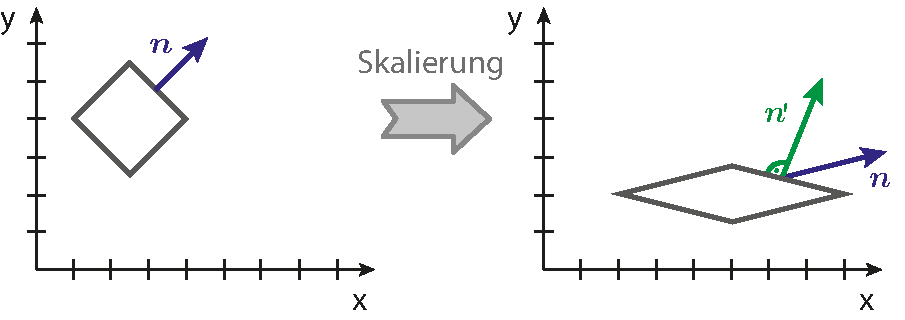
\includegraphics[width=1\textwidth]{./img/transformation/normale_skalierung.pdf}
    \caption{Die Raute und ihre Normale $\boldsymbol{n}$ werden auf die gleiche Art und Weise transformiert und zwar auf die doppelte Breite und halbe Höhe skaliert. Nach der Skalierung steht $\boldsymbol{n}$ nicht mehr orthogonal auf der Oberfläche. Die korrekte Normale ist $\boldsymbol{n'}$. D.h. die Normale muss bei der Transformation gesondert behandelt werden.
    }
    \label{fig:normale_skalierung}
\end{figure}

%Auch am Schnittpunkt eines transformierten Objekts wird eine Normale \( \vv{n'} \) benötigt.
Momentan ist der "`Raytracer"' in der Lage den Schnittpunkt eines Primärstrahls mit einem transformierten Objekt zu berechnen. Was fehlt, ist die Normale an diesem Schnittpunkt. Problematisch ist die Tatsache, dass die Normalen jeweils nur für die untransformierten Objekte erzeugt werden (s. Kapitel~\ref{ch:obj_schnitt}).
Abb.~\ref{fig:normale_skalierung} verdeutlicht, dass auf diese Normalen nicht einfach die gleiche Transformation angewendet werden kann, die für das Objekt verwendet wurde. Denn nach der Skalierung steht \( \boldsymbol{n} \) in der Abbildung nicht länger senkrecht auf der Oberfläche des Objekts. Die korrekte Normale ist \( \boldsymbol{n'} \). 

Nach \cite{pharrhumphrey2010Physically} (S. 87) ist es das Ziel, \( \boldsymbol{n} \) derart zu transformieren, dass dabei \( \boldsymbol{n'} \) herauskommt. 
Zur Veranschaulichung stellt man sich eine ebene Oberfläche vor, in der zwei Punkte liegen. Die Differenz der Punkte bildet einen Tangentialvektor. Nach einer Transformation liegen die Punkte weiterhin in der ebenen Oberfläche und somit auch der Tangentialvektor.
Das heißt, wird auf den Tangentialvektor einer Oberfläche die gleiche Transformation angewandt, wie auf die Oberfläche selbst, bleibt er weiterhin Tangentialvektor.

Nun bedient man sich der Tatsache, dass die Normale \( \boldsymbol{n} \) senkrecht auf dem Tangentialvektor \( \boldsymbol{t} \) steht und damit ihr Skalarprodukt Null ergibt. Nach der Transformation muss auch die neue Normale \( \boldsymbol{n'} \) senkrecht auf dem transformierten Tangentialvektor \( \boldsymbol{t'} \) stehen. Dabei ist \( \boldsymbol{T} \) die Transformation, die auf die Oberfläche und den Tangentialvektor angewendet wird, und \( \boldsymbol{S} \) ist die gesuchte Transformation, die auf die Normale anzuwenden ist.
Somit ist:

\begin{align*}  
    0 &=  \boldsymbol{t'} \cdot \boldsymbol{n'} \\
    0 &=  \left( \boldsymbol{S} \cdot \boldsymbol{n} \right) \cdot \left( \boldsymbol{T} \cdot \boldsymbol{t} \right) \\
    0 &= \left( \boldsymbol{S} \cdot \boldsymbol{n} \right)^\intercal \left( \boldsymbol{T} \cdot \boldsymbol{t} \right)  \qquad \qquad \text{siehe Gleichung \ref{eq:skalarprodukt}} \\
    0 &= \boldsymbol{n}^\intercal \left( \boldsymbol{S}^\intercal \cdot \boldsymbol{T} \cdot \boldsymbol{t} \right)
\end{align*}

Wie bereits erwähnt, gilt die Prämisse  \( \boldsymbol{n}^\intercal \boldsymbol{t} = 0 \), d.h. \( \boldsymbol{S}^\intercal \cdot \boldsymbol{T} \) muss letztendlich einfach aus der Gleichung verschwinden und somit die Einheitsmatrix ergeben. Damit \( \boldsymbol{S}^\intercal \cdot \boldsymbol{T} = \mathds{1} \) gilt, muss \( \boldsymbol{S}^\intercal = \boldsymbol{T}^{-1} \) sein.
Eine letzte Umformung liefert das Ergebnis \( \boldsymbol{S} = (\boldsymbol{T}^{-1})^\intercal \). Um eine Normale also korrekt zu transformieren, muss sie mit der transponierten Inversen der ursprünglichen Transformationsmatrix transformiert werden.




%0 &= \vv{t} \cdot \vv{n} \\

%Siehe "`Raytracing from Ground Up"' S. 217


\chapter{Schattierung} \label{ch:schattierung}


Bis jetzt ist der "`Raytracer"' in der Lage Strahlen in eine Szene bestehend aus Objekten auszusenden und Schnittpunkte zu berechnen. An diesen Schnittpunkten muss nun ein Farbwert berechnet werden, der anschließend dem PEE zugewiesen wird, welches vom Strahl durchdrungen wurde. Den Vorgang zur Berechnung des Farbwerts bezeichnet man in der Computergrafik als Schattierung. 


\section{Die Rendergleichung}

Beim "`Raytracing"' erfolgt die Schattierung eines Objekts durch Lösung der Rendergleichung. Der Farbwert ergibt sich aus der Summe aller, über der Hemisphäre eines Schnittpunktes, einfallender Strahldichten. Dabei entscheidet der Einfallwinkel und der Schnittpunkt, welche Frequenzanteile, einer einfallenden Strahldichte, mit welcher Intensität entlang eines Primärstrahls auf das PEE reflektiert wird. Zur Modellierung dieses Sachverhalts verwendet man bidirektionale Reflektanzverteilungsfunktionen (engl. bidirectional reflectance distribution function, BRDF\abk{BRDF}{Bidirectional reflectance distribution function}). Die BRDF ist damit maßgeblich für die Oberflächeneigenschaft und somit für die Schattierung eines Objekts verantwortlich.

\begin{equation}
    L_o(\boldsymbol{p}, \boldsymbol{\omega_o}) = L_e(\boldsymbol{p}, \boldsymbol{\omega_o}) + \int_{2\pi^+} f_r(\boldsymbol{p}, \boldsymbol{\omega_i}, \boldsymbol{\omega_o}) \cdot L_i(\boldsymbol{p}, \boldsymbol{\omega_i}) \cos(\theta_i) \mathrm{d} \boldsymbol{\omega_i}
    \label{eq:rendergleichung}
\end{equation}

Gleichung~\ref{eq:rendergleichung} zeigt die Rendergleichung. Der Term \( L_o(\boldsymbol{p}, \boldsymbol{\omega_o}) \) steht dabei für die, aus der Oberfläche austretende Strahldichte. Dieser Term ist wie bereits erwähnt abhängig vom Schnittpunkt \( \boldsymbol{p} \) und der Strahlrichtung \( \boldsymbol{\omega_o} \), die der inversen Richtung des Primärstrahls entspricht. Der Term \( L_e(\boldsymbol{p}, \boldsymbol{\omega_o}) \) wird für Oberflächen benötigt, die selbst Licht emittieren. Der restliche Summenteil der ausgehenden Strahldichte ergibt sich, indem man über alle möglichen Strahlrichtungen \( \boldsymbol{\omega_i} \) in der Hemisphäre integriert, die sich über dem Schnittpunkt \( \boldsymbol{p} \) befindet. Die einfallenden Strahldichten \( L_i(\boldsymbol{p}, \boldsymbol{\omega_i}) \), werden wie erwähnt durch die BRDF \( f_r(\boldsymbol{p}, \boldsymbol{\omega_i}, \boldsymbol{\omega_o}) \) skaliert. Zuletzt fehlt noch der Ausdruck \( \cos(\theta_i) \), der dafür sorgt, dass flacher einfallende Strahldichten einen geringeren Beitrag zur ausgehenden Strahldichte leisten, als steiler einfallende. Der Winkel \( \theta_i \) lässt sich aus der Normale \( \boldsymbol{n} \) am Schnittpunkt \( \boldsymbol{p} \) und der Strahlrichtung \( \boldsymbol{\omega_i} \), eines einfallenden Strahls, berechnen.

Die Rendergleichung kann in der Regel nicht analytisch gelöst werden und muss daher approximiert werden. Eine Variante besteht darin, Strahlen gemäß einer Verteilung (z.B. gleichverteilt) über der Hemisphäre, in die Szene zu schicken, um konkrete Werte für \( L_i(\boldsymbol{p}, \boldsymbol{\omega_i}) \) zu berechnen. Trifft einer dieser Strahlen auf ein Objekt wird das Verfahren rekursiv fortgesetzt, bis eine Lichtquelle getroffen wird. Dieses Vorgehen nennt man "`Path Tracing"' und kann für kleine Lichtquellen sehr lange dauern, da Strahlen diese nur selten treffen. Für unendlich viele ausgesandte Strahlen, stellt "`Path Tracing"' jedoch eine korrekte Lösung der Rendergleichung da.

Beim "`Whitted Raytracing"' wird hingegen für jeden Primärstrahl, der ein Objekt trifft, der Term \( L_i(\boldsymbol{p}, \boldsymbol{\omega_i)} \) berechnet, indem Strahlen nur zu allen in der Szene befindlichen Lichtquellen ausgesandt werden. Diese Methode ist deutlich schneller, stellt jedoch nur eine sehr ungenaue Approximation der Rendergleichung da. Die folgenden Abschnitte zeigen, wie Objekte nach der "`Whitted"' Methode schattiert werden können.


\section{Matte Oberfläche}

\begin{wrapfigure}{r}{0.5\textwidth}    
    \vspace{-15pt}
    \centering
    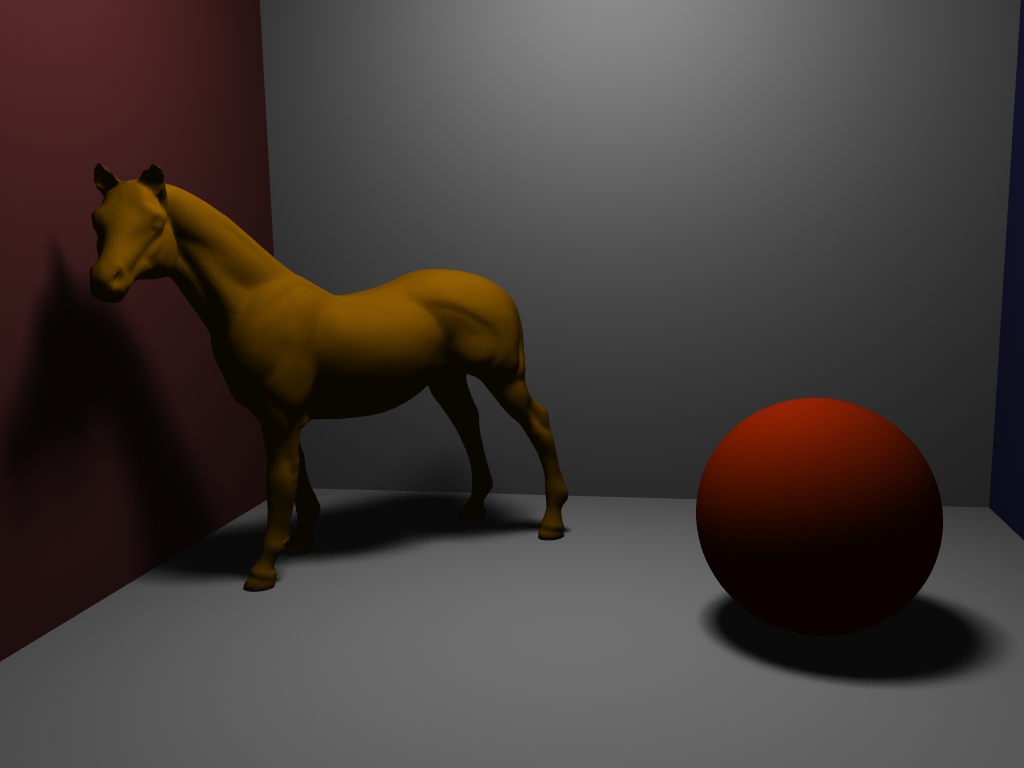
\includegraphics[width=0.49\textwidth]{img/schattierung/matte_0,05_0,85.png}
    \vspace{-10pt}
    \caption{Pferdemodell und Kugel in einer Box  }
    \label{fig:matte_0,05_0,85.png}
\end{wrapfigure}

Matte oder "`lambertsche"' Oberflächen besitzen eine sehr einfache Schattierung. Sie bestehen im Wesentlichen aus zwei Komponenten und zwar aus einem ambienten und einem diffusen Term:

\( f_{matt}(\boldsymbol{p}, \boldsymbol{\omega_i}, \boldsymbol{\omega_o}) = k_a \cdot c_a + k_d \cdot c_d \)

 Der ambiente Term ist unabhängig vom Austrittswinkel \( \omega_o \) und dem Einfallswinkel \( \omega_i \). Da beim "`Whitted Raytracing"' die Lichtausbreitung zwischen nicht-Licht emittierenden Objekten fehlt, soll er den Eindruck von vorhandenem Umgebungslicht vermitteln. Bei \( k_a \) handelt es sich um den ambienten Reflexionskoeffizienten \( k_a \). Er bestimmt den Anteil der ambienten Komponente in der ausgehenden Strahldichte. Die Materialkonstante \( c_a \), sorgt für die Färbung des Objekts, indem sie bestimmte Spektren absorbiert und andere reflektiert. Wird \( c_a \) als RGB-Wert dargestellt, so entspricht dies einer Multiplikation mit dem RGB-Wert der einfallenden Strahldichte. Für die diffuse Komponente sind die Bedeutungen von \( k_d \text{ und } c_d \) analog. In der gerasterten Computergrafik wird für die matte Oberflächen noch ein Term benötigt, der die Intensität eines Farbwertes skaliert, je nachdem wie flach oder steil ein Strahl von der Lichtquelle auf die Oberfläche trifft. Beim "`Raytracing"' ist dieser Sachverhalt bereits durch \( \cos{\theta_i} \), in der Rendergleichung, modelliert
 

\section{Spekulare Oberfläche - Phong}

Für spekulare Oberflächen muss die matte Schattierung um eine weitere Komponente ergänzt werden. Diese Komponente ist verantwortlich für die Darstellung von Glanzpunkten und wird Phong-Komponente genannt:

\begin{equation*}
f_{phong}(\boldsymbol{p}, \boldsymbol{\omega_i}, \boldsymbol{\omega_o}) = f_{matt}(\boldsymbol{p}, \boldsymbol{\omega_i}, \boldsymbol{\omega_o}) + \left( \frac{\boldsymbol{\omega_o} \cdot \boldsymbol{r} }{|\boldsymbol{\omega_o}| \cdot |\boldsymbol{r}|} \right)^n \cdot k_p \cdot c_p
\end{equation*}

Bei den Konstanten \( k_p \) und \( c_p \) handelt es sich um den  Reflexionskoeffizienten und die Materialkonstante. Diese werden mit einem Term multipliziert, der den Winkel zwischen ausgehender Strahlrichtung \( \boldsymbol{\omega_o} \) und einem Vektor \( \boldsymbol{r} \) berechnet. Bei \( \boldsymbol{r} \) handelt es sich um die perfekte Reflexionsrichtung, eines einfallenden Lichtstrahls. Er wird erzeugt durch 

\( \boldsymbol{r} = -\boldsymbol{\omega_i} \cdot 2 \cdot (\boldsymbol{n} \cdot \boldsymbol{\omega_i}) \cdot \boldsymbol{n}\), wobei Normale \( \boldsymbol{n} \) und \( \boldsymbol{\omega_i} \) normalisiert sein müssen. Je weiter der Winkel zwischen Beobachter und perfekt reflektiertem Lichtstrahl ist, desto geringer ist der Anteil der Phong-Komponenten an der ausgehenden Strahldichte. Der Exponent \( n \) wird dazu verwendet die Ausdehnung der Glanzpunkte festzulegen, wie Abb.~\ref{fig:phong_30} und Abb.~\ref{fig:phong_100} zeigen. Je größer \( n \) ist, desto konzentrierter erscheinen die Glanzpunkte.

\begin{minipage}[t]{0.48\textwidth}
    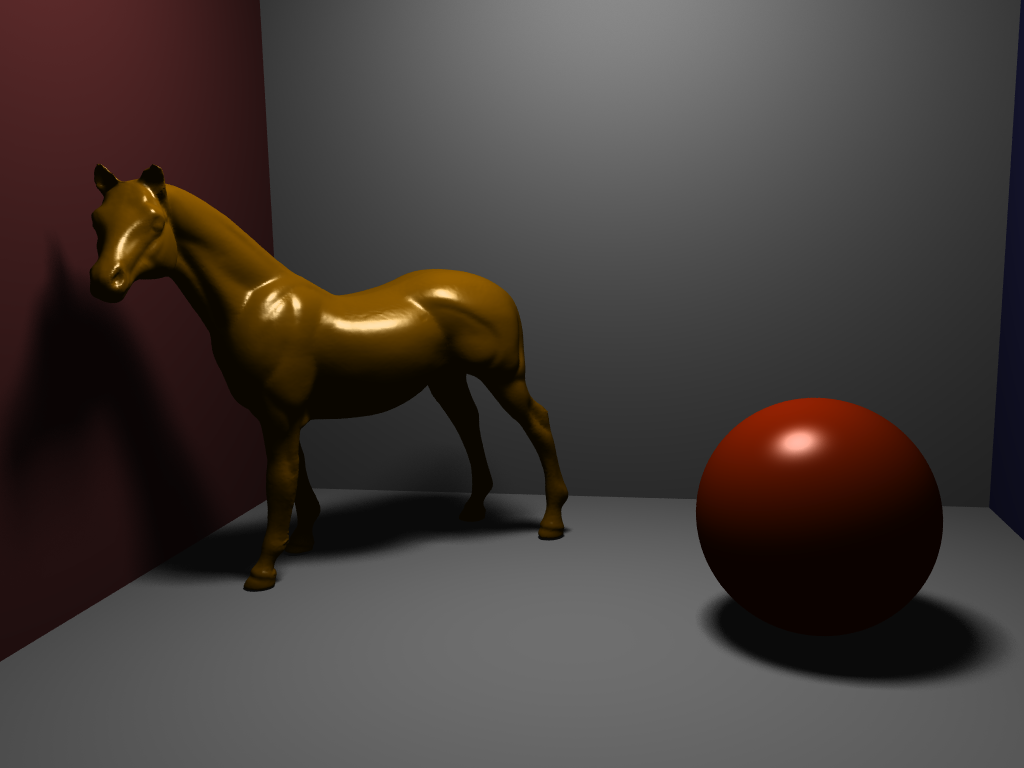
\includegraphics[width=\textwidth]{./img/schattierung/phong_30.png}
    \captionof{figure}{Pferd und Kugel mit spekularer Oberfläche. Die Größen der Glanzpunkte ergeben sich durch den Exponenten $n=30$.}
    \label{fig:phong_30}
\end{minipage}
\begin{minipage}[t]{0.48\textwidth}
    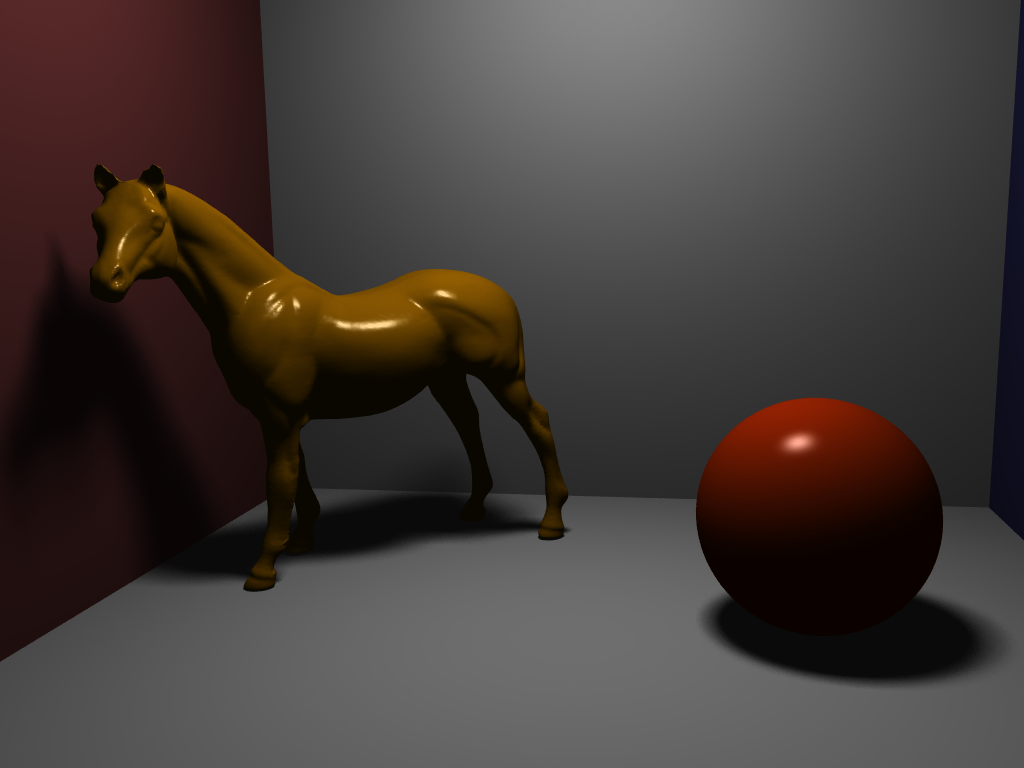
\includegraphics[width=\textwidth]{./img/schattierung/phong_100.png}
    \captionof{figure}{Pferd und Kugel mit spekularer Oberfläche. Die Größen der Glanzpunkte ergeben sich durch den Exponenten $n=100$.}
    \label{fig:phong_100}
\end{minipage}

\section{Spiegelnde Oberfläche}

Die Spiegeloberflächen aus Abb.~\ref{fig:rmirror_100exp} und Abb.~\ref{fig:mirror} stellen eine Erweiterung der Phong-Schattierung da. Jedoch sollten die ambiente, diffuse und Phong-Komponente sehr dezent eingesetzt werden. Perfekte Reflexion kann umgesetzt werden, indem ein Strahl in Richtung perfekter Reflexionsrichtung \( \boldsymbol{r} \) ausgesandt wird. Trifft er ein anderes Objekt, wird dort am Schnittpunkt die Schattierungsberechnung durchgeführt und die Strahldichte berechnet. Die dort berechnete Strahldichte kann dann anhand eines weiteren additiven Terms bestehend aus Reflexionskoeffizient und Materialkonstante verändert und zur ausgehenden Strahldichte der perfekt spiegelnden Oberfläche hinzugefügt werden.

Abb.~\ref{fig:phong_30} zeigt eine matt spiegelnde Oberfläche. Dies erreicht man, indem man Strahlen konisch verteilt, entlang von \( \boldsymbol{r} \) in die Szene schickt.



\begin{minipage}[t]{0.48\textwidth}
    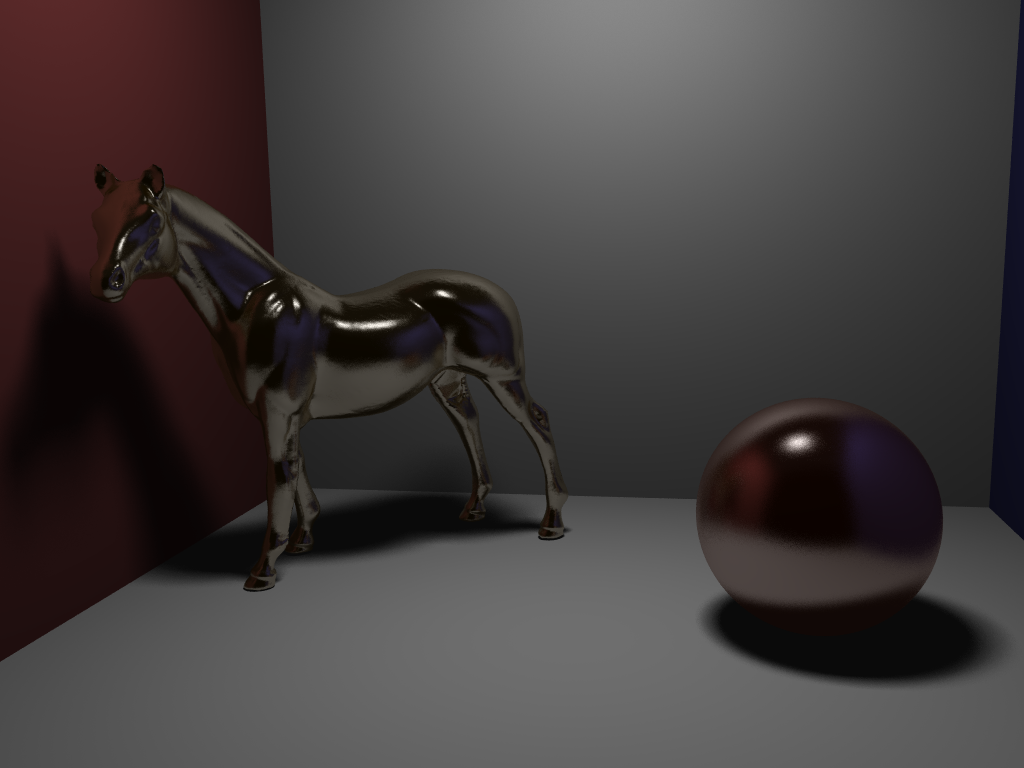
\includegraphics[width=\textwidth]{./img/schattierung/rmirror_100exp.png}
    \captionof{figure}{Das Aussehen der matt spiegelnden Oberflächen wird erzeugt, indem Strahlen konisch um die perfekte Reflexionsrichtung $\boldsymbol{r}$ in die Szene geschickt werden.}
    \label{fig:rmirror_100exp}
\end{minipage}
\begin{minipage}[t]{0.48\textwidth}
    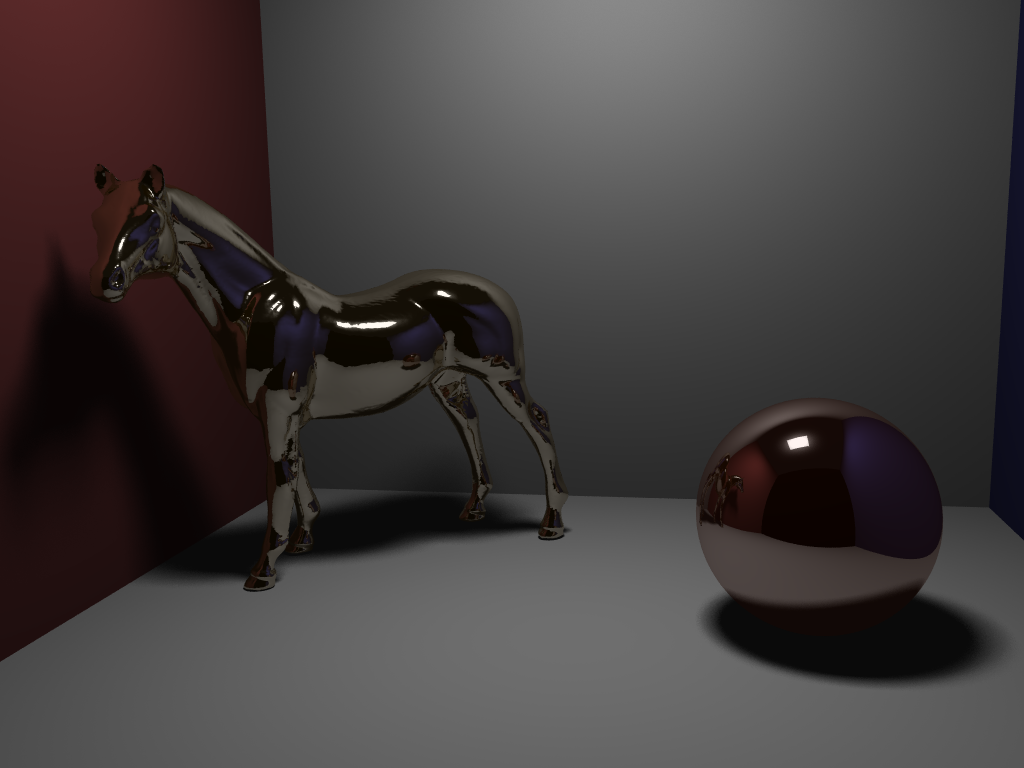
\includegraphics[width=\textwidth]{./img/schattierung/mirror.png}
    \captionof{figure}{Das Aussehen der perfekt spiegelnden Oberflächen wird erzeugt, indem Strahlen entlang der perfekten Reflexionsrichtung $\boldsymbol{r}$ in die Szene geschickt werden.}
    \label{fig:mirror}
\end{minipage}


\section{Dielektrikum}

Bei Dielektrika handelt es sich um Materialien, die Anteile eines eintreffenden Lichtstrahls brechen und reflektieren. Jedes Dielektrikum besitzt einen Brechungsindex. Mit Hilfe des Snelliusschen Brechungsgesetz und des Brechungsindex kann bestimmt werden, in welche Richtung ein Strahl gebrochen wird, wenn er vom umgebenden Medium in das Dielektrikum übergeht. Wenn ein Strahl zu flach auf die Oberfläche auftrifft, kann es passieren, dass er komplett reflektiert wird und muss dann wie bei perfekt spiegelnden Oberflächen behandelt werden. Man spricht in diesem Fall von Totalreflexion. Findet keine Totalreflexion statt, wird ein Teil des Strahls gebrochen und ein Teil reflektiert. Durch die Fresnelschen Formeln kann dann bestimmt werden, aus welchen Anteilen der Strahldichte des gebrochenen Strahls und des reflektierten Strahls, sich die ausgehende Strahldichte zusammensetzt.  

\begin{minipage}[t]{0.48\textwidth}
    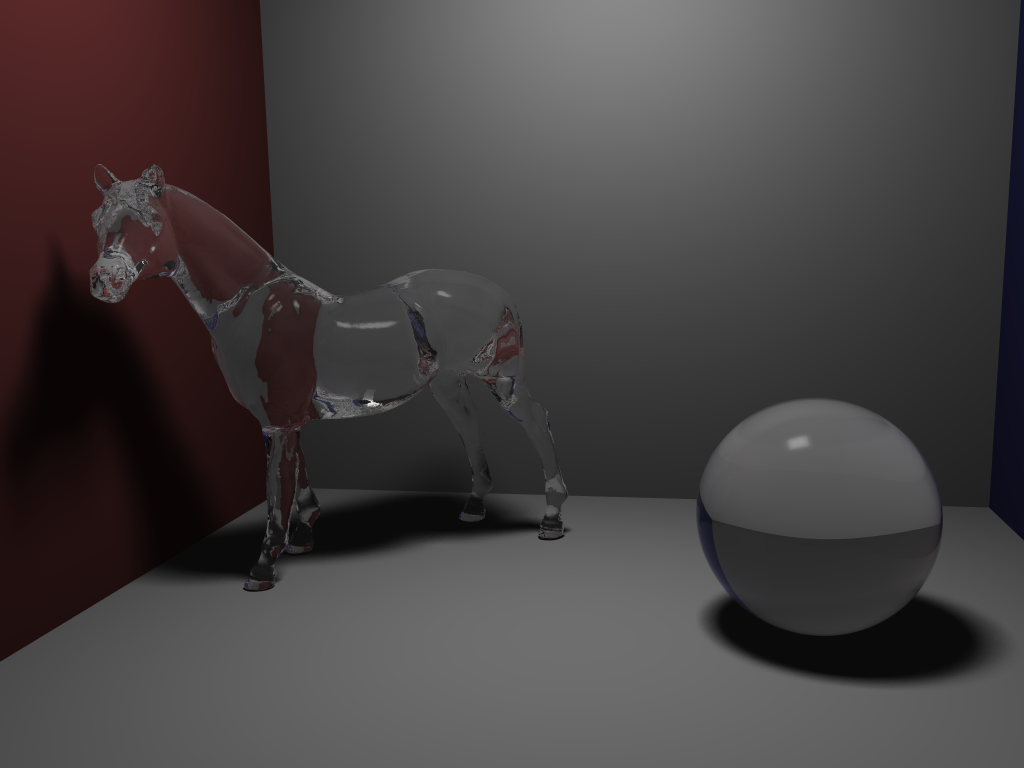
\includegraphics[width=\textwidth]{./img/schattierung/dielectric_1_1,3.png}
    \captionof{figure}{Dielektrika mit einem Brechungsindex von 1,3. Dies entspricht näherungsweise dem Übergang von Luft zu Eis}
    \label{fig:dielectric_1_1,3.png}
\end{minipage}
\begin{minipage}[t]{0.48\textwidth}
    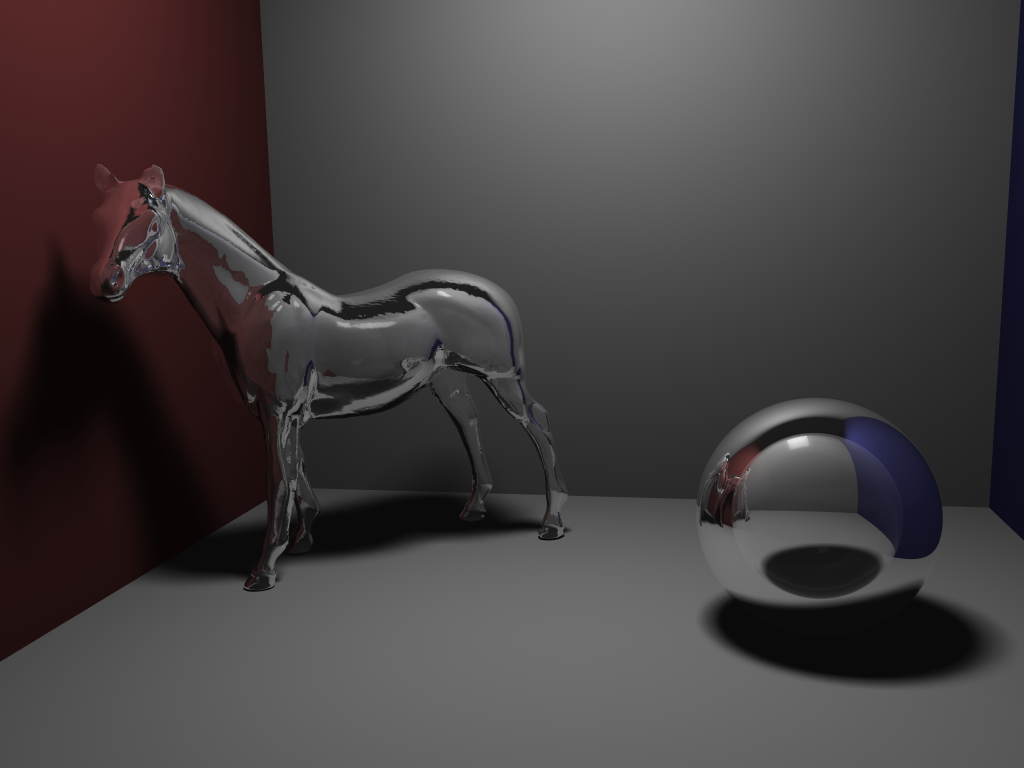
\includegraphics[width=\textwidth]{./img/schattierung/dielectric_1_0,7.png}
    \captionof{figure}{Dielektrika mit einem Brechungsindex von 0,75. Dies entspricht näherungsweise dem Übergang von Wasser zu Luft}
    \label{fig:dielectric_1_0,7.png}
\end{minipage}



\chapter{Triangulierte Objekte}

Komplexe Objekte wie der Stanford Bunny bestehen aus einem Polygonnetz. Die einfachste Form des Polygons ist das Dreieck und die so zusammengesetzten Objekte sind triangulierte Objekte.
Im Abschn.~\ref{sec:dreieck} wurde bereits gezeigt wie man den Schnittest und die Berechnung der Normalen für Dreiecke durchführt.
Die naive Erweiterung um triangulierte Objekte beim "`Raytracing"' verwenden zu können, besteht darin, für jedes einzelne Dreieck im Dreiecksnetz eben diese Schritte durchzuführen. Wenn das triangulierte Objekt nur aus wenigen Dreiecken besteht, ist diese Vorgehensweise noch durchführbar. Der Stanford Buddha besteht jedoch aus über einer Million Dreiecke, wovon jedes mit jedem Strahl getestet werden müsste. In Kapitel~\ref{ch:beschleunigung} werden deshalb Beschleunigungsstrukturen vorgestellt, um die Anzahl durchgeführter Schnitttests zu reduzieren.

\section{Das OBJ-Format}

Zur Repräsentation eines Dreiecksnetzes existieren Dateiformate wie das OBJ-Format von Wavefront~\cite{reddy2015obj}. Das OBJ-Format erlaubt eine kompakte Darstellung des Polygonnetzes, indem alle vorkommenden Punkte aufgelistet werden und die jeweiligen Polygone durch Referenzierung der Punktindices definiert werden. Dadurch werden Punkte, die von mehreren Polygonen verwendet werden, nicht mehrmals gespeichert.

Das nun folgende Beispiel zeigt die Definition eines in der xy-Achse liegenden Quadrats. Es ist im Ursprung zentriert, hat eine Kantenlänge von 2 und ist aus zwei Dreiecken zusammengesetzt.

\begin{verbatim}
# Definition eines Quadrats im OBJ Format

v  -1.0   1.0  0.0
v  -1.0  -1.0  0.0
v   1.0   1.0  0.0
v   1.0  -1.0  0.0
# 4 Punkte

vn 0.0000 -0.0000 1.0000
# 1 Normale

f 1//1 2//1 3//1     # Punktindex/Texturkoordinate/Normalenindex
f 4//1 3//1 2//1     # Punktindex/Texturkoordinate/Normalenindex
# 2 Dreiecksfächen
\end{verbatim}

Die OBJ-Datei wird von oben nach unten abgearbeitet. Kommentare werden durch \texttt{\#} gekennzeichnet.
Definitionen werden durch Bezeichner eingeleitet und erhalten einen impliziten Index beginnend mit 1.
Als erstes werden Punkte definiert, eingeleitet durch den Bezeichner \texttt{v}. Die nachfolgenden Zahlen stehen für die x, y und z-Komponente eines Punktes im dreidimensionalem Raum. Der erste definierte Punkt erhält den Index 1. Für folgende Punkte wird der Index jeweils inkrementiert.
Als nächstes folgt die Definition von Punktnormalen, gekennzeichnet durch den Bezeichner \texttt{vn}. Die drei nachfolgenden Zahlen entsprechen wieder den einzelnen Komponenten. Die Angabe von Punktnormalen ist optional. 
Sollten keine Punktnormalen definiert sein, wird für jedes Dreieck eine Dreiecksnormale berechnet, wie in Abschn.~\ref{sec:dreieck} gezeigt.

 Zuletzt folgt die Definition der Polygone, in diesem Fall Dreiecke, durch \texttt{f}. Die nachfolgenden Spalten folgen dem Schema \texttt{Punktindex/Texturkoordinatenindex/Normalenindex}. Im angegebenen Beispiel wird das erste Dreieck somit aus dem ersten, zweiten und dritten Punkt erzeugt. Texturkoordinaten werden zur Einfachheit im Beispiel ausgelassen. In Kapitel~\ref{ch:texturierung} wird aber noch konkret gezeigt, wie Texturkoordinaten aussehen. Zuletzt wird jedem Dreieckspunkt eine optionale Punktnormale durch \texttt{Normalenindex} zugewiesen. Falls keine Punktnormalen in der OBJ-Datei enthalten sind, können diese nachträglich berechnet werden wie der nachfolgende Abschnitt zeigt.
 
 Das vorgestellte (Minimal-) Beispiel ist so einfach, dass es noch ohne Probleme händisch erstellt werden kann. Für sehr komplexe Objekte, die z.B. aus mehreren zehntausend Polygonen bestehen und mehrere Texturen verwenden, benötigt man eine 3D-Modellierungssoftware zur Erstellung einer solchen Datei, weshalb "`3ds Max"' von "`Autodesk"' zur Erstellung und Bearbeitung von 3D-Modellen benutzt wird. Zum Laden von 3D-Modellen kommt neben dem selbstgeschriebenen OBJ-Parser noch die quelloffene Bibliothek "`Assimp"' zum Einsatz, die eine Vielzahl an Formaten für 3D-Modelle unterstützt.


\section{Facettierte und glatte Schattierung} \label{sec:facetierte_und_glatte_schattierung}

Abb.~\ref{fig:konstante_schattierung} zeigt den "`Stanford Bunny"' in facettierter Schattierung. Diese Art der Schattierung erhält man, wenn man pro Dreieck eine einzige Dreiecksnormale verwendet. Die einzelnen Dreiecke sind dann gut erkennbar, da sich die Farbe innerhalb eines Dreiecks nicht großartig verändert. Dies hat folgenden Grund: Unabhängig von der Lage des Schnittpunkts wird immer die gleiche Dreiecksnormale verwendet. Die einzige, für die Schattierung relevante Komponente, die sich mit der Lage des Schnittpunkts ändert, ist der Einfallswinkel der Lichtstrahlen. Bei entsprechend kleinen Dreiecken ändert sich der Einfallswinkel des Lichtstrahls nur geringfügig, wodurch der Eindruck entsteht, dass das Dreieck einfarbig ist.
Um den "`Bunny"' so zu schattieren, wurde eine OBJ-Datei geladen, die lediglich Polygone sowie entsprechende Punkte enthält. Da im OBJ-Format die Polygone mit einem Umlaufsinn gegen den Uhrzeigersinn definiert werden, kann eine Dreiecksnormale direkt nach der Vorgehensweise aus Abschn.~\ref{sec:dreieck} berechnet werden.

Im Gegensatz dazu zeigt Abb.~\ref{fig:glatte_schattierung} wie eine glatte Schattierung erzielt werden kann, indem sich die Normale abhängig vom Schnittpunkt ändert. Dies geschieht durch Interpolation der Punktnormalen. Seien \( \boldsymbol{n_0}, \boldsymbol{n_1} \text{ und } \boldsymbol{n_2} \) die Punktnormalen, die den Dreieckspunkten (z.B. durch die OBJ-Datei) zugewiesen sind. Bei Durchführung des Dreieckschnitttests erhält man die baryzentrischen Koordinaten \( \beta \text{ und } \gamma \), die die Position des Schnittpunkts innerhalb des Dreiecks widerspiegeln (siehe Abschn.\ref{sec:dreieck}). Diese Koordinaten werden nun zur Berechnung der Normalen am Schnittpunkt \( \boldsymbol{n_{\boldsymbol{r}}} \) benutzt:

\begin{equation*}
    \boldsymbol{n_{\boldsymbol{r}}} = (1 - \beta - \gamma) \cdot \boldsymbol{n_0} + \beta \cdot \boldsymbol{n_1} + \gamma \cdot \boldsymbol{n_2}
\end{equation*}

Wie bereits erwähnt, ist die Angabe der Punktnormalen optional und so ist es möglich, dass keine in der OBJ-Datei vorhanden sind. Es gibt jedoch die Möglichkeit, diese nachträglich zu berechnen. Falls keine Punktnormalen vorhanden sind, wird für jedes Dreieck eine Dreicksnormale berechnet. Möchte man nun für einen bestimmten Punkt die Punktnormale berechnen, so iteriert man über alle angrenzenden Dreiecke, die diesen Punkt verwenden, und summiert deren Dreiecksnormalen auf. Die resultierende Normale ist jedoch kein Einheitsvektor mehr und muss normalisiert werden, falls diese Eigenschaft gefordert ist.


%\begin{algorithm}[H]
%    \caption{Berechne Punktnormale für Dreickspunkt \( \boldsymbol{p_0} \)}
%    \label{alg:punktnormale}
%    \begin{algorithmic}[1]
%        \State \( \vv{n}_{res} \gets \vv{0} \) 
%        \For {each \( \text{Polygon } poly \in polygon\_enthalt\_p_0 \)}
%        \State \( \vv{n}_{res} \gets \vv{n}_{res} + dreicksnormale\_von(poly) \)
%        \EndFor
%        \State \( \vv{n}_{res} \gets \vv{n}_{res} \cdot |\vv{n}_{res}|^{-1} \)
%    \end{algorithmic}
%\end{algorithm}
%\todo{Algorithum muss definitiv formal besser aufgeschrieben werden.}
%



\begin{minipage}[t]{0.48\textwidth}
    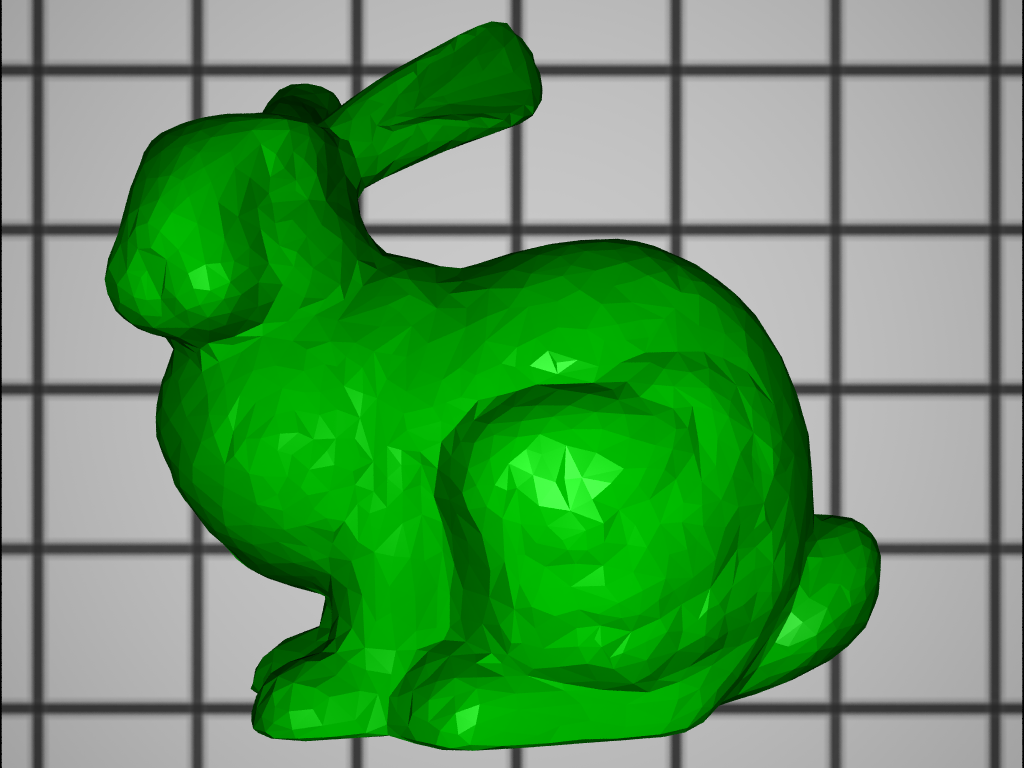
\includegraphics[width=\textwidth]{./img/triangulierte_objekte/konstante_schattierung.png}
    \captionof{figure}{Verwendung nur einer Normalen pro Dreieck führt zu facettierter Schattierung}
    \label{fig:konstante_schattierung}
\end{minipage}
\begin{minipage}[t]{0.48\textwidth}
    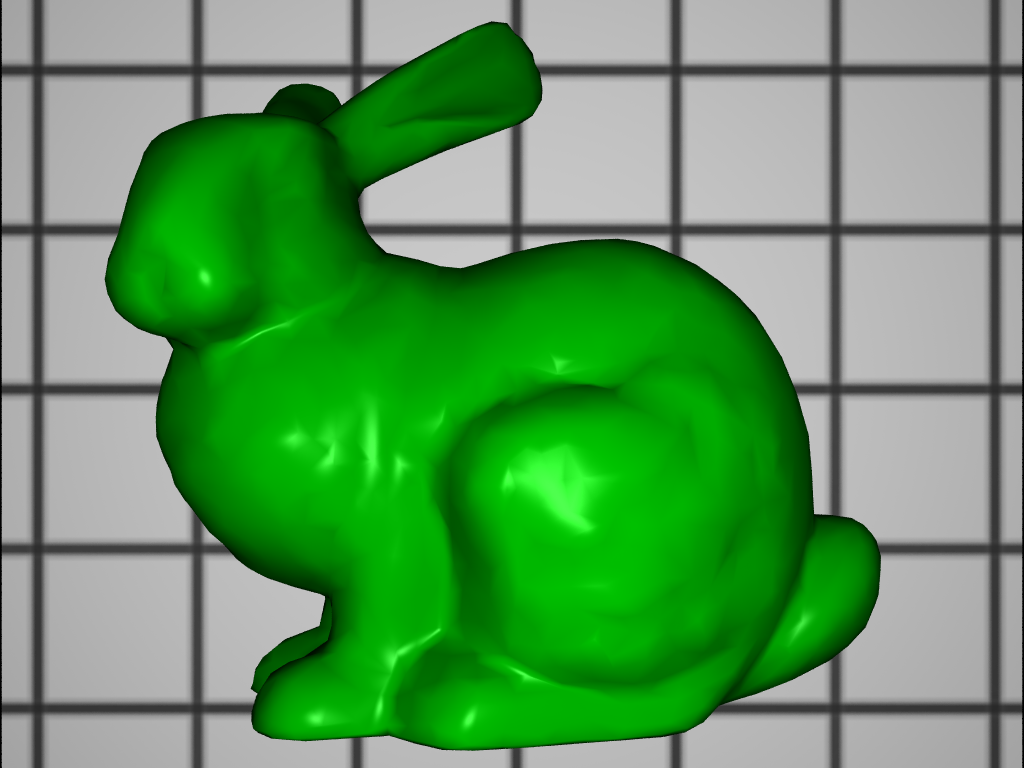
\includegraphics[width=\textwidth]{./img/triangulierte_objekte/glatte_schattierung.png}
    \captionof{figure}{Einbeziehung und Mittelwertbildung benachbarter Dreiecksnormalen sorgt für glattere Schattierung}
    \label{fig:glatte_schattierung}
\end{minipage}









\section{Instanziierung}

Durch Instanziierung kann ein einzelnes Polygonnetz für mehrere Objekte verwendet werden. Programmiertechnisch erzeugt man dazu eine Klasse, die eine Referenz auf das Polygonnetz enthält. Des weiteren speichert die Klasse eine Transformationsmatrix und deren Inverse, sowie Oberflächeneigenschaften in Form eines Materials. Mit dieser Ausstattung ist es möglich, zu prüfende Strahlen zu transformieren und den transformierten Strahl mit dem Polygonnetz zu testen. Dadurch lässt sich ein möglicher Schnittpunkt ermitteln. Die dabei erhaltene Normale wird entsprechend transformiert und zur Berechnung der Schattierung, durch das ebenfalls gespeicherte Material, verwendet. So lässt sich auf speicherplatzsparende Art ein und dasselbe Polygonnetz mit unterschiedlichen Transformationen und Schattierungen darstellen. Zudem wird die Laufzeit verkürzt, da das Polygonnetz nicht mehrmals geladen werden muss. Noch schwerer ins Gewicht fällt das Erzeugen einer Beschleunigungsstruktur, was dadurch ebenfalls reduziert wird (s. Unterabschnitt~\ref{subs:geschwindigkeitsmessung} ).


\chapter{Schnellere Schnitttests durch Beschleunigungsstrukturen} \label{ch:beschleunigung}

Bisher wurde jeder Primärstrahl mit jedem schnitttestfähigen Objekt in der Szene getestet.
Spätestens mit der Einführung von triangulierten Objekten, die durchaus aus mehreren hunderttausend Dreiecken bestehen können, ist diese Vorgehensweise nicht mehr praktikabel, da so die Laufzeit linear mit der Anzahl an schnitttestfähigen Objekten zunimmt. Mit den folgenden Beschleunigungsstrukturen lässt sich die Anzahl der Schnitttests durch eine obere Grenze von \( O(log(n)) \) beschränken, wobei \( n \) die Anzahl schnitttestfähiger Objekte ist. Der Fokus wird dabei auf die "`bounding interval hierarchy"' (BIH\abk{BIH}{Bounding interval hierarchy}) \cite{wachter2006InsRayTraBouIntHie} gelegt.

\section{Übersicht}

Es existieren bereits verschiedene Ansätze, um die Schnitttests mit der Geometrie zu beschleunigen. Häufig geht es darum, frühzeitig die Objekte auszuschließen, mit denen sicher kein Schnitt vorliegt. Ein erster Schritt, um dies zu erreichen, gelingt durch die Verwendung von Hüllkörpern. Das sind meist sehr einfache Körper wie Kugeln oder Quader, für die ein Schnitttest sehr schnell durchgeführt werden kann. Schneidet ein Strahl den Hüllkörper nicht, so muss auch nicht die umschlossene Geometrie überprüft werden. Schneidet jedoch ein Strahl den Hüllkörper, muss die komplette Geometrie auf Schnitte überprüft werden. Falsch-positive Fälle liegen vor, wenn ein Hüllkörper geschnitten wird, aber kein Schnitt mit der Geometrie gefunden wird. Um solche unnötigen Tests zu vermeiden, sollte der Hüllkörper die Geometrie möglichst eng umschließen.


Ihr volles Potential entfalten Hüllkörper in Kombination mit räumlichen Hierarchien (engl. spatial hierarchy). Dazu gehört z.B. die "`BVH"'\abk{BVH}{Bounding volume hierarchy} (engl. "`bounding volume hierarchy"'). Ziel ist es, die gesamte Geometrie entsprechend ihrer Lage im Raum zu sortieren und in einer Baumstruktur abzulegen. Man beginnt an der Wurzel und erzeugt einen Hüllkörper für die gesamte Geometrie. Nun teilt man die Geometrie anhand eines bestimmten Kriteriums auf, z.B. gleichmäßige Aufteilung der Geometrie auf beide Kindknoten und erzeugt für die aufgeteilte Geometrie kleinere Hüllkörper, die in den Kindknoten gespeichert werden. Dies wird solange fortgesetzt, bis ein Abbruchkriterium erfüllt ist, wie z.B. maximale Tiefe des Baumes oder eine bestimmte Anzahl an Objekten im Knoten, für die keine weitere Teilung durchgeführt wird. Knoten, die eine dieser Bedingungen erfüllen, nennt man Blätter. In ihnen werden Referenzen auf diese Objekte gespeichert. Die Schwierigkeit besteht darin, die Geometrie so aufzuteilen, dass bei der Traversierung des Baumes möglichst nur ein Pfad bearbeitet werden muss. Die Traversierung des Baums beginnt an der Wurzel,
mit dem größten Hüllkörper und wird rekursiv mit Kindknoten fortgesetzt, die ebenfalls vom Strahl geschnitten werden.
 

%Auch bei gleichmäßigen Gittern (engl. uniform grids) kommen Hüllkörper zum Einsatz, werden jedoch nur zur Konstruktion gebraucht.
%Das Gitter besteht aus gleich großen Zellen. 
%
% die aus gleich großen Zellen bestehen. Manche dieser Zellen beinhalten Objekte und andere sind leer. Ein Strahl durchdringt nun nacheinander, die hintereinander liegenden Zellen und führt den Schnitttest nur mit Objekten durch, die sich in der jeweiligen Zelle befinden.

Einen anderen Ansatz verfolgen die "`kd-Trees"'. Hier geht es darum, den Raum so aufzuteilen (engl. space partitioning), dass bei der Traversierung des "`kd-Trees"' möglichst große Raumteile ausgeschlossen werden können und somit die darin befindlichen Objekte nicht getestet werden müssen. Kritisch für die Laufzeit ist hierbei die Wahl der Trennebenen, die den Raum rekursiv in zwei kleinere Bereiche aufteilen. Bei der Traversierung wird getestet, welcher der beiden Raumteile bzw., ob beide Raumteile vom Strahl durchdrungen werden, indem ein Strahl-Ebenen Schnitttest mit der Trennebenen durchgeführt wird. Sobald man einen Raumteil erreicht, der nicht mehr weiter unterteilt ist, werden die darin befindlichen Objekte mit dem Strahl auf Schnitte getestet.


\section{Die "`bounding interval hierarchy"'}

Die Entscheidung auf die "`bounding interval hierarchy"' (BIH) als Beschleunigungsstruktur zu setzen, beruht auf mehreren Gründen.

Für kd-Tree kann vorab nicht entschieden werden, wieviel Speicherplatz im RAM benötigt wird, da Objekte in mehreren Raumteilen referenziert werden können. Denn der Raum kann so geteilt werden, dass ein Objekt in beiden Seiten des geteilten Raumes liegt. Des weiteren birgt das die Problematik von numerischen Instabilitäten und erfordert evt. die Verwendung eines Benachrichtungssystems, um Objekte nicht mehrfach auf Schnitte überprüfen zu müssen.

BVH sind, was die Performance anbelangt, den gut konstruierten kd-Trees unterlegen,
aber dafür recht einfach zu bauen. Der Speicherbedarf kann besser abgeschätzt werden (linear in anzahl der Objekten).
Sie sind numerisch stabiler, da kein Strahl-Ebenen Schnitt, sondern nur min-max Operationen angewendet werden.

Die BIH vereinigt viele der Vorteile beider Methoden, ohne unter deren Nachteile zu leiden.
So sind BIH sehr leicht zu verstehen und zu implementieren, was die Fehleranfälligkeit reduziert. Ihre Konstruktion ähnelt der von BVH, wodurch sie sehr schnell erzeugt werden kann. Damit ist sie für dynamische Szenen oder Echtzeit "`Raytracing"' verwendbar. Die Traversierung verläuft hingegen sehr ähnlich zu der von kd-Trees. Damit ist die BIH nicht nur konkurrenzfähig zu den Traversierungszeiten von kd-Trees, sondern schlägt diese sogar in bestimmten Szenen~\cite{wachter2006InsRayTraBouIntHie}. Jedes Objekt wird exakt einmal in einem Blatt referenziert. Dadurch ist der benötigte Speicherverbrauch vorab berechenbar und es werden keine Benachrichtigungssysteme benötigt.

\subsection{Konstruktion}

Zur Konstruktion der BIH werden "`axis aligned bounding boxes"' (AABB\abk{AABB}{Axis aligned bounding boxes}) benötigt. Das sind quaderförmige Hüllkörper, deren Kanten parallel zu den Achsen des globalen Koordinatensystems verlaufen. Die Repräsentation einer AABB gestaltet sich auf Grund dieser Eigenschaft relativ einfach. Es reicht aus für jede Achse die Ausdehnung der AABB durch einen minimalen und maximalen Wert festzulegen. Die Bezeichner dafür lauten \( min_{x,y,z}, max_{x,y,z} \), wobei das Subskript die entsprechende Achse referenziert.
 
Ein schneller Strahl-AABB Schnitttest (s. Alg.~\ref{alg:strahl_aabb} ) wird in \cite{pharrhumphrey2010Physically} vorgestellt. Dieser liefert, für den Parameter \( t \) aus der Strahlgleichung, die Werte \( t_{min} \) für den nächsten Schnittpunkt und \( t_{max} \) für den entfernteren. Es sei erwähnt, dass der Code so konstruiert wurde, dass er die Besonderheiten der IEEE Spezifikation für Gleitkommazahlen berücksichtigt. So ist die Ausführung des Codes auch dann noch korrekt, wenn eine Komponente \( {\boldsymbol{d}.i } \) des Strahlrichtungsvektor 0 ist und \( d_{inv} \) somit die Werte \( -\infty \) oder \( \infty \) annimmt. Das Gleiche gilt für den Fall, dass der Strahlursprung in einer der Seiten der AABB liegt. Dann kann \( t_{near} \) oder \( t_{far} \) in Zeile 6 und 7 den Wert "`NaN"' annehmen, da \( {\boldsymbol{o}.i } \cdot d_{inv} \) zu "`\( 0 \cdot \pm\infty  \)"' wird. Da Vergleichsoperationen mit "`NaN"' immer "`false"' liefern (außer man vergleicht 2 "`NaN"' miteinander) bleiben \( t_0 \) und \( t_1 \) unverändert.

\begin{algorithm}[H]
    \caption{Schnittest Strahl-AABB}
    \label{alg:strahl_aabb}
    \begin{algorithmic}[1]
        \State \( t_0 \gets -\infty \)
        \State \( t_1 \gets \infty \)\\
        
        \For {\textbf{each} \( i \in \{x,y,z\} \)}
            \State \( d_{inv} \gets 1 / {\boldsymbol{d}.i } \)	\Comment \( \boldsymbol{d}.i  \) \( \equiv \) Komponenten des Strahlrichtungsvektors
            \State \( t_{near} \gets min_i - {\boldsymbol{o}.i } \cdot d_{inv}  \)	\Comment \( {\boldsymbol{o}.i } \) \( \equiv \) Komponenten des Strahlursprungs
            \State \( t_{far} \gets max_i - {\boldsymbol{o}.i } \cdot d_{inv} \)
            
            \If{\( t_{near} > t_{far} \)}
                \State{\( \text{swap}(t_{near}, t_{far}) \)}	\Comment Vertauschen der Werte von \( t_{near} \text{ und } t_{far} \)
            \EndIf
            \If{\( t_{near} > t_0 \)}
                \State \( t_0 \gets t_{near} \)
            \EndIf
            \If{\( t_{far} < t_1 \)}
            \State \( t_1 \gets t_{far} \)
            \EndIf
            \If{\( t_0 > t_1 \)}
                \State\Return{\textbf{false}}
            \EndIf
        \EndFor\\
        
        \State \( t_{min} \gets t_0 \)
        \State \( t_{max} \gets t_1 \)
        \State\Return{\textbf{true}}
       
    \end{algorithmic}
\end{algorithm}

Ziel ist es nun, die Objekte der Szene in einer Baumstruktur abzulegen. Es beginnt damit, eine globale AABB zu erzeugen, die alle Objekte der Szene umfasst. Um die Objekte partitionieren zu können, muss eine Trennebene gefunden werden. Das Konstruktionsverfahren der BIH teilt dazu die globale AABB mittig durch sogenannte Trennebenenkandidaten entlang der längsten Achse auf, wie Abb.~\ref{fig:bih_konstruktion} -a zeigt. Dabei werden nur die Seiten weiter unterteilt, in denen sich auch tatsächlich Objekte befinden. So zeigt Abb.~\ref{fig:bih_konstruktion} -b die final verwendeten Trennebenen, leere Räume sind nicht weiter unterteilt.

\begin{figure}[ht]
    \centering
    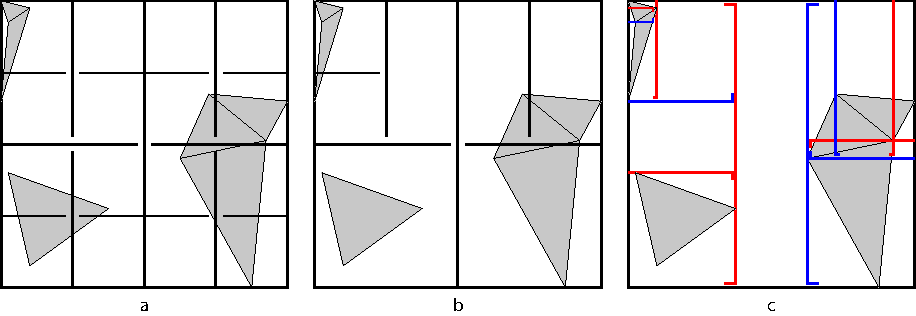
\includegraphics[width=1\textwidth]{./img/beschleunigungsstrukturen/bih_konstruktion.pdf}
    \caption{a) Rekursive Unterteilung der Szene anhand von Trennebenenkandidaten. Die jeweils längste Achse wird mittig durch einen Trennebenenkandidat geteilt. b) Tatsächliche Aufteilung des Raums nach Ablegen der Objekte in Blättern. Leere Räume benötigen keine weitere Unterteilung. c) Rote Klammern zeigen die maximale Ausdehnung der Objekte des linken Kindknoten entlang der geteilten Achse. Blaue Klammern zeigen minimale Ausdehnung der Objekte des rechten Kindknoten. \protect\footnotemark}
    \label{fig:bih_konstruktion}
\end{figure}

\footnotetext{Quelle: \cite{wachter2006InsRayTraBouIntHie} / Seite 5}


Nach Festlegung einer Trennebene wird überprüft, welche Objekte sich links bzw. rechts von der Trennebene befinden. Eine einfache Vorgehensweise besteht darin eine AABB um die zu prüfenden Objekte zu legen und ihren Mittelpunkt zu berechnen. Da die Trennebene immer parallel zu einer der 3 Achsen des globalen Koordinatensystems verläuft, kann die entsprechende Komponente des Mittelpunkts verwendet werden, um die Zuordnung durchzuführen.
Nun wird ein innerer Knoten erzeugt und dieses Schema rekursiv fortgesetzt, bis eine Abbruchbedingung, wie maximale Tiefe des Baumes oder minimale Anzahl zu teilender Objekte erreicht ist. Ist eine Abbruchbedingung erreicht, wird ein Blatt erzeugt und die vom Raumteil des Blattes umschlossenen Objekte im Blatt vermerkt.

Die allgemeine Definition eines Knotens sieht in der Programmiersprache C wie folgt aus und dient zur Erzeugung von inneren Knoten, wie auch Blättern \cite{wachter2006InsRayTraBouIntHie}. Im Folgenden wird erläutert, welche Informationen in inneren Knoten und Blättern gespeichert werden: 

\begin{lstlisting}[language=C,escapeinside=``]
typdef struct
{
  int Index; //LSB: (x=00,y=01,z=10)-Achse oder Blatt(11)
  union
  {
    int   Items;   // Nur Bl`ä`tter
    float Clip[2]; // Nur innere Knoten
  };
} BIH_Node;
\end{lstlisting}


Die beiden niederwertigsten Bit (engl. "`least significant Bit"' LSB \abk{LSB}{Least significant bit}) der Variable "`Index"' werden dazu benutzt, anzuzeigen, ob es sich um ein Blatt handelt, falls nicht, handelt es sich um einen innerer Knoten und die beiden LSB zeigen an, entlang welcher Achse des globalen Koordinatensystems die Unterteilung stattfindet. Die Bedeutung der einzelnen Werte kann der Definition entnommen werden. Die restlichen Bit der Variable "`Index"' werden dazu verwendet, einen Zeiger auf die beiden Kindknoten zu speichern, falls es sich um einen inneren Knoten handelt. Blätter speichern hingegen einen Zeiger auf eine Liste dem Blatt zugeordneter Objekte.
Innere Blätter müssen zudem noch 2 Trennebenen speichern. Dabei handelt es sich nicht um die Trennebenenkandidaten, die zur Partitionierung der Objekte verwendet wurden! Vielmehr wird in Clip[0] die maximale Ausdehnung der Objekte im linken Kindknoten entlang der Koordinatenachse gespeichert und in Clip[1] die minimale Ausdehnung der Objekte im rechten Kindknoten. In Abb.~\ref{fig:bih_konstruktion} -c sind diese Trennebenen durch rote und blaue Klammern gekennzeichnet. Blätter müssen keine Trennebenen speichern, deshalb wird ein "`union"' verwendet, um den ohnehin verbrauchten Speicherplatz für das Speichern der Anzahl im Blatt enthaltener Objekte zu verwenden.


\subsection{Traversierung}

Die Traversierung beginnt damit, dass ein Schnitttest gemäß Algorithmus~\ref*{alg:strahl_aabb} mit der globalen AABB durchgeführt wird. Wenn die globale AABB nicht geschnitten wird, liegt auch kein Schnitt mit der Geometrie vor und die Traversierung endet. Ansonsten erhält man für den Parameter \( t \) der Strahlgleichung die Werte \( t_{min} \) für den nächsten Schnittpunkt und \( t_{max} \) für den entfernteren.
Jetzt wird der Wurzelknoten der BIH zusammen mit \( t_{min} \) und \( t_{max} \) auf einen Stapel (engl. "`stack"') gelegt und die nachfolgenden Anweisungen durchgeführt, bis der Stapel leer ist oder frühzeitig der nächste Schnitt gefunden wurde, wozu die Variable \( t_{Schnitt} \) benötigt wird. Diese wird zu Beginn auf einen sehr großen Wert gesetzt.

\begin{enumerate}
    \item Entnehme den obersten Knoten und die zugehörigen Werte \( t_{min} \) und \( t_{max} \) vom Stapel.
    \item Teste ob \( t_{Schnitt} < t_{min} \), falls ja, fahre mit Anweisung 1. fort. Denn der aktuell zu betrachtende Raumteil ist weiter entfernt als der bisher nächste gefundene Schnittpunkt. Somit können die darin liegenden Objekte unmöglich einen näheren Schnittpunkt liefern.
    \item Teste ob es sich beim aktuellen Knoten um ein Blatt handelt, falls ja, führe Schnitttests mit allen enthaltenen Objekten durch und weise \( t_{Schnitt} \) den minimalen Strahlgleichungsparameter zu. Fahre mit Anweisung 1. fort.
    \item Weise das linke Kind des aktuellen Knotens der Variable \( {KnotenNah } \) und das rechte der Variable \( KnotenFern \) zu. Teste ob die Komponente der Strahlrichtung \( \boldsymbol{d} \), die der Trennebene des aktuellen Knotens entspricht, negativ ist. Falls ja, weise \( KnotenNah \) das rechte und \( KnotenFern \) das linke Kind zu. Somit ist sicher gestellt, dass der Raumteil, der später vom Strahl geschnitten wird, zuerst in den Stapel gelangt und damit nach dem Raumteil betrachtet wird, der zuerst geschnitten wird.
    \item Führe einen Strahl-Ebenen Schnitt mit \( cNah = (\verb|Clip[0]|
    - \boldsymbol{p}.i) * {\boldsymbol{d}.i}^{-1} \) durch, wobei \verb|Clip[0]| die Position der Trennebene des linken Teilraumes beinhaltet (s. Definition BIH\_Node). \( \boldsymbol{p}.i \) und \( \boldsymbol{d}.i \) sind die Komponenten des Strahlursprungs und der Strahlrichtung, wobei \( i \) die Achse ist, auf die sich die Trennebene des aktuellen Knotens bezieht. Berechne \( cFern \) analog, nur mit der Trennebene des rechten Teilraums \verb|Clip[1]| anstelle von \verb|Clip[0]|. Falls \( \boldsymbol{d}.i \)  negativ ist, wurde in Anweisung 4. \( KnotenNah \) und \( KnotenFern \) vertauscht, also tausche auch die Werte von \( cNah \) und \( cFern \), falls \( \boldsymbol{d}.i \) negativ ist.
    \item Teste ob \( cFern \le t_{tmin} \), falls ja, setze \( t_{min} \) auf das Maximum, gebildet aus \( t_{min} \text{ und } cFern\), um den fernen Teilraum weiter einzugrenzen und lege \( KnotenFern \) zusammen mit \( t_{max} \) und dem angepassten \( t_{min} \) auf den Stapel.
    \item Teste ob \( (0 \le cNah) \land (t_{min} \le cNah) \), falls ja, setze \( t_{max} \) auf das Minimum gebildet aus \( t_{max} \) und \( cNah \), um den nahen Teilraum weiter einzugrenzen und lege \( KnotenNah \) zusammen mit \( t_{min} \) und dem angepassten \( t_{max} \) auf den Stapel.
    \item Überprüfe, ob der Stapel leer ist, falls ja, fahre mit Anweisung 9. fort. Ansonsten fahre mit Anweisung 1. fort.
    \item Wenn sich \( t_{Schnitt} \) vom initial zugewiesen Wert unterscheidet, kam ein Schnitt zustande, ansonsten nicht. \( t_{Schnitt} \), verwendet als Strahlgleichungsparameter, liefert dann den nächsten Schnitt. Ende.
    
\end{enumerate}

Ein Detail ist in der beschriebenen Traversierung noch nicht beachtet worden. Und zwar können Strahlen parallel zu den Koordinatenebenen verlaufen, wodurch mindestens eine Komponente der Strahlrichtung \( \boldsymbol{d} \) gleich 0 sein wird. Damit liefert der Schnitttest aus Anweisung 5. die Werte \( \infty \) und \( -\infty \) wegen Division durch 0, bzw. "`NaN"' wenn die Komponente \( \boldsymbol{p}.i \) des Strahlursprungs mit einer der Trennebenenpositionen aus \verb|Clip[0]| oder \verb|Clip[1]| übereinstimmt, wegen der Berechung \( \frac{0}{0} \). Diese Spezialfälle müssen noch gesondert überprüft werden.


\subsection{Geschwindigkeitsmessung}\label{subs:geschwindigkeitsmessung}

Ziel dieses Abschnittes ist es, die Geschwindigkeit der BIH anhand zweier Szenen zu demonstrieren und den Unterschied zur Ausführung des "`Raytracers"' ohne Beschleunigungsstruktur zu zeigen. Gemessen wird die Zeit, die die BIH zur Konstruktion benötigt, sowie die Laufzeit des reinen Renderprozesses, dessen größter Anteil in der Traversierung der BIH besteht. Die Messung findet auf einem "`Intel i5-3570k"' Prozessor statt. Die zu rendernden Szenen besitzen eine Auflösung von \( 800 \times 800 \) Pixel. Jeder Pixel wird anhand eines Primärstrahls durch den Mittelpunkt berechnet.

\begin{minipage}[t]{0.48\textwidth}
    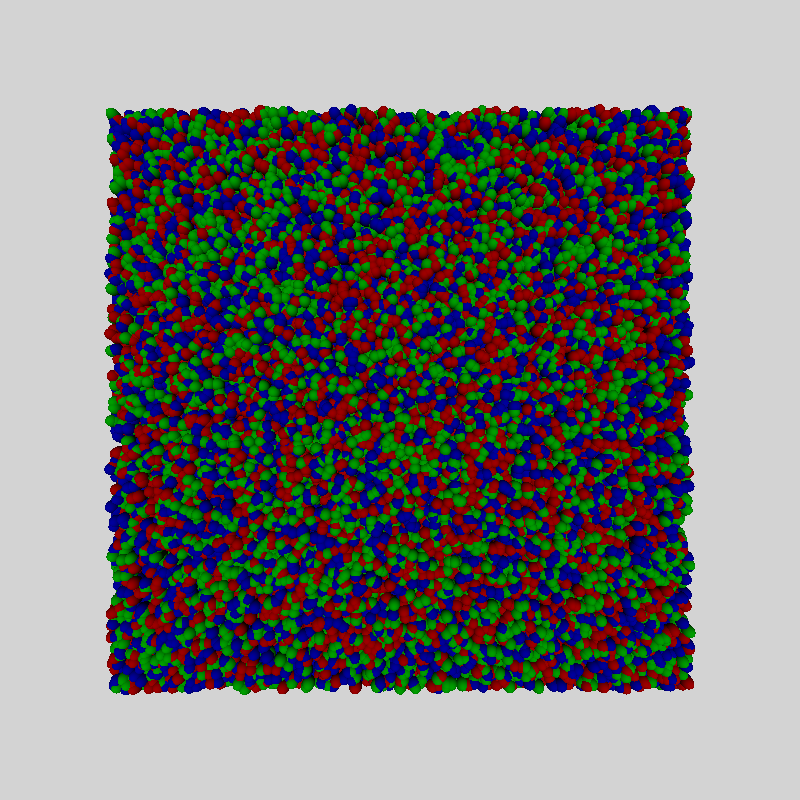
\includegraphics[width=\textwidth]{./img/beschleunigungsstrukturen/1mio_spheres_800x800pxl.png}
    \captionof{figure}{Die Testszene "`Kugeln"' zeigt 1 Million, innerhalb eines Würfels mit der Kantenlänge 9, gleichverteilte Kugeln. Die Auflösung des Bilds beträgt $800 \times 800$ Pixel. }
    \label{fig:1mio_spheres}
\end{minipage}
\begin{minipage}[t]{0.48\textwidth}
    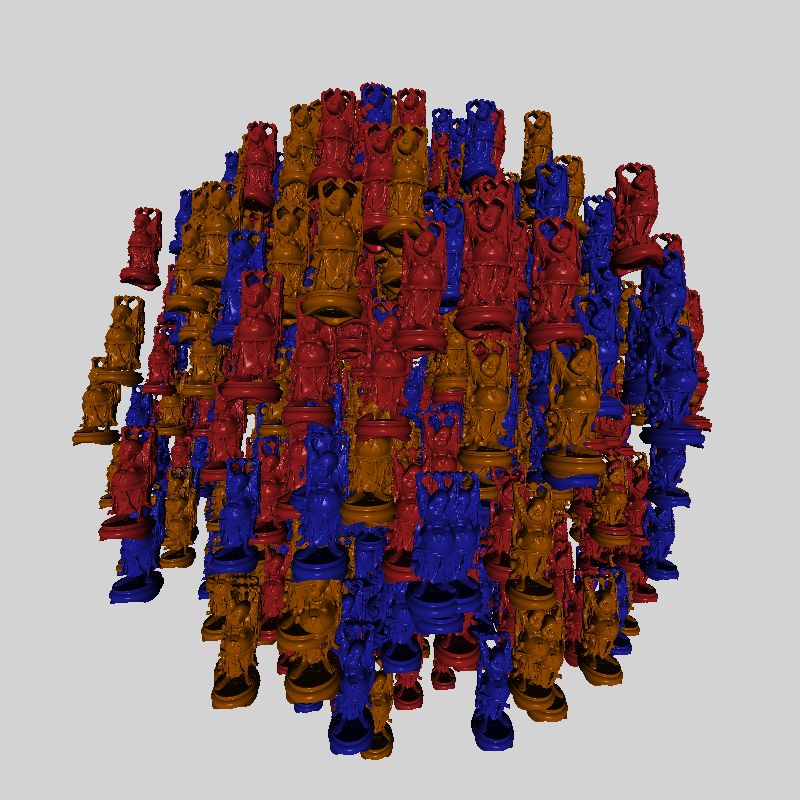
\includegraphics[width=\textwidth]{./img/beschleunigungsstrukturen/1k_buddhas_800x800.png}
    \captionof{figure}{Die Testszene "`Buddhas"' zeigt 1000, innerhalb einer Kugel mit Radius 9, gleichverteilte Stanford Buddhas. Die Auflösung des Bilds beträgt $800 \times 800$ Pixel.}
    \label{fig:1k_buddhas}
\end{minipage}

In der Testszene "`Kugeln"' (s. Abb.~\ref{fig:1mio_spheres} ) werden Kugeln innerhalb eines Würfels mit Kantenlänge 9 gleichverteilt. Es wird die Zeit in Sekunden gemessen, die es dauert die BIH zu erzeugen sowie zu traversieren. Die Erzeugung der BIH findet dabei immer "`single threaded"' statt, wohingegen die Traversierung mit mehreren "`threads"' durchgeführt werden kann. In der Traversierungszeit steckt zudem noch die Zeit, die zur Schattierung der Objekte benötigt wird. Um diese nicht unnötig aufzublähen, wird nur eine Phong-Schattierung verwendet.


 

\begin{figure}[ht]
    \centering
    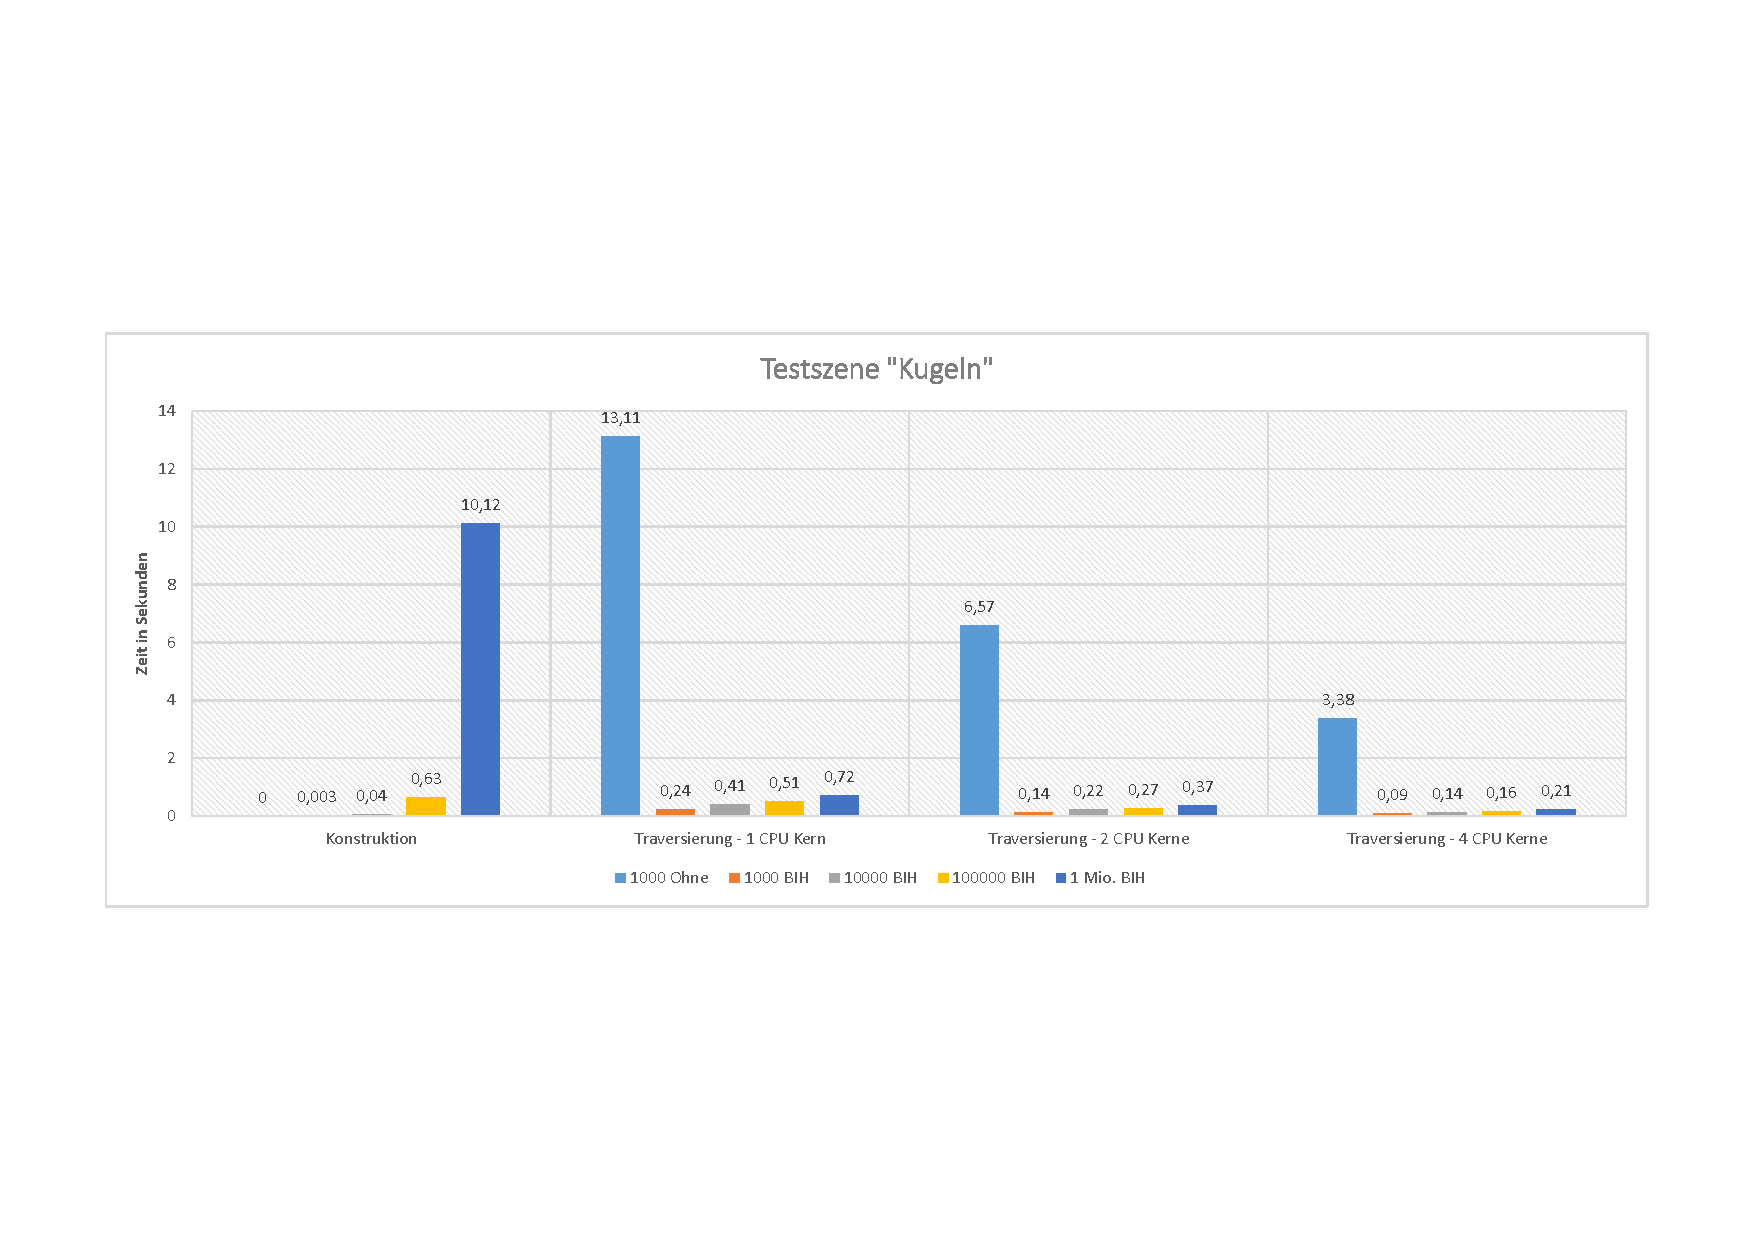
\includegraphics[width=1\textwidth]{./img/beschleunigungsstrukturen/Laufzeiten_Kugelszene.pdf}
    \caption{Zeitmessung in Sekunden der Testszene "`Kugeln"'. Das Diagramm ist unterteilt in Segmente, zur Zeitmessung der Konstruktion sowie der Traversierung der BIH. Die Konstruktion findet immer auf einem CPU Kern statt, wohingegen die Traversierung mit 1, 2 und 4 Kernen durchgeführt wird. Die Balken innerhalb eines Segments stehen für die Anzahl der Objekte in der Szene und zeigen an, ob die BIH verwendet wurde oder nicht ("`Ohne"').  }
    \label{fig:laufzeiten_kugel}
\end{figure}
\begin{figure}[ht]
    \centering
    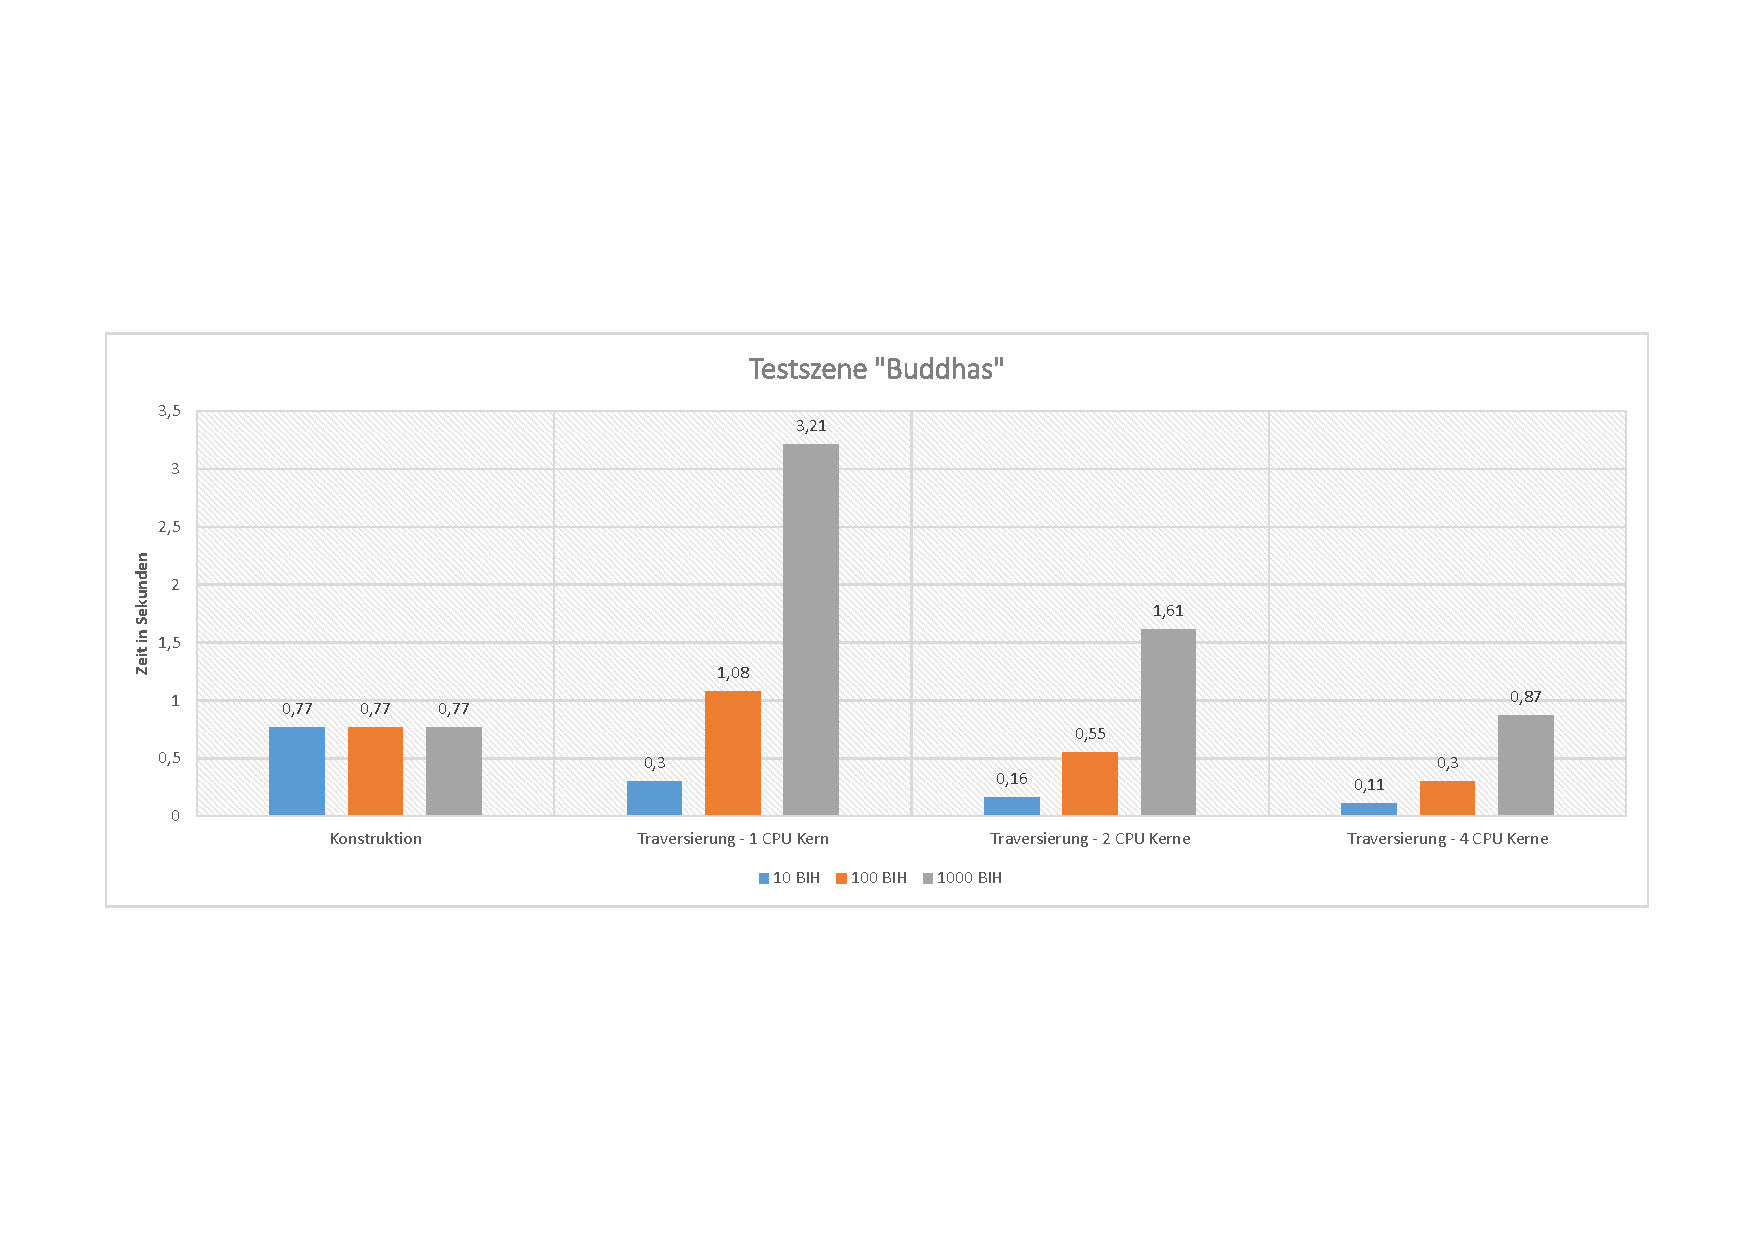
\includegraphics[width=1\textwidth]{./img/beschleunigungsstrukturen/Laufzeiten_Buddhaszene.pdf}
    \caption{Zeitmessung in Sekunden der Testszene "`Buddhas"'. Das Diagramm ist unterteilt in Segmente, zur Zeitmessung der Konstruktion sowie der Traversierung der BIH. Die Konstruktion findet immer auf einem CPU Kern statt, wohingegen die Traversierung mit 1, 2 und 4 Kernen durchgeführt wird. Die Balken innerhalb eines Segments stehen für die Anzahl der Objekte in der Szene. Zum Rendern der Buddhas wurde Instanziierung verwendet, wodurch die Konstruktionszeit gleich bleibt.}
    \label{fig:laufzeiten_buddha}
\end{figure}

Die Messungen aus Abb.~\ref{fig:laufzeiten_kugel} werden für 1000, 10000, 100000 und 1 Million Objekte durchgeführt. Die Diagrammsegmente unterteilen sich in Konstruktionszeit sowie Traversierungszeiten, durchgeführt mit unterschiedlicher Anzahl an "`threads"'. Es zeigt sich bereits bei 1000 Objekten, dass es äußerst unpraktikabel ist jeden Primärstrahl mit jedem Objekt auf Schnitt zu testen. Betrachtet man den Fall, in dem die Konstruktion sowie Traversierung nur auf einem CPU Kern stattfindet, so ist die BIH bei 1 Million Objekte trotz Konstruktionszeit von 10,12 Sekunden und einer Traversierungszeit von 0,72 Sekunden immer noch schneller als der naive Ansatz ohne Beschleunigungsstruktur, der 13,11 Sekunden für 1000 Objekte benötigt.

Für den Stanford Buddha, bestehend aus 100000 Dreiecken, würde das Rendern ohne Beschleunigungsstruktur viel zu lange dauern, weshalb die Zeitmessung nur mit BIH durchgeführt wurde. Die Konstruktionszeiten aus Abb.~\ref{fig:laufzeiten_buddha} zeigen eine Besonderheit, denn sie bleiben konstant, trotz steigender Anzahl Buddhas in der Szene. Dies ist der bereits angesprochenen Instanziierung geschuldet. Es wird nur einmal das Dreiecksnetz des Buddhas geladen und dafür eine BIH erzeugt. Die verschiedenen Instanzen speichern dann eine Referenz auf das Dreiecksnetz und verwenden unterschiedliche Transformationsmatrizen und Materialien.

Ein weiterer Fakt, der aus den Diagrammen hervorgeht, ist die Tatsache, dass die Konstruktionszeit der BIH in \( O(n \cdot log(n)) \) und die Traversierungszeit in \( O(log(n)) \) liegt, wobei \( n \) die Anzahl schnitttestfähiger Objekte ist. Des weiteren zeigt sich, dass "`Raytracer"' prädestiniert dazu sind, parallelisiert zu werden. In der Testszene "`Buddhas"' lässt sich die Traversierungszeit für 1000 Buddhas durch die Verwendung von 4 CPU Kernen fast um Faktor 4 verringern (auf 0,87 Sekunden), im Vergleich zur seriellen Ausführung (3,21 Sekunden) (s.Abb.~\ref{fig:laufzeiten_buddha} ).
 


\chapter{Texturierung} \label{ch:texturierung}

\begin{wrapfigure}[16]{r}{0.44\textwidth}    
    \vspace{-15pt}
    \centering
    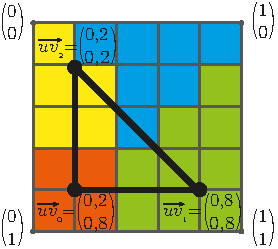
\includegraphics[width=0.43\textwidth]{img/texturierung/textur.pdf}
    \vspace{-10pt}
    \caption{Textur als 2D-Array mit uv-Koordinaten als Spaltenvektor der Form $ \binom{u}{v} \in \mathds{R}^2 $ }
    \label{fig:textur}
\end{wrapfigure}



In der Realität besitzen Objekte eine Vielzahl an geometrischen und materiellen Feinstrukturen. Beispiele dafür sind die Maserung bei Holz oder Kratzer und Unebenheiten in Oberflächen. Es wäre viel zu aufwendig, all diese Feinheiten durch ein polygonales Modell nachzubilden. Um Objekte dennoch mit solchen Details ausstatten zu können, verwendet die Computergrafik Texturen.

Abstrakt betrachtet, handelt es sich bei einer Textur um eine Funktion, die einen Punkt in der xy-Ebene auf ein Texturelement, auch Texel genannt, abbildet. Meistens werden Texturen durch Bitmaps realisiert. Diese bestehen aus einem 2D-Array in dem Farbwerte z.B. in RGB-Darstellung gespeichert werden. Daher werden Texel oft mit Farbwerten assoziiert. Tatsächlich können Texel auch andere Dinge repräsentieren wie z.B. Normalen oder Skalare. Dies hängt davon ab, wie Texturen umgesetzt werden und wie ein Texel interpretiert wird. Ein RGB-Farbwert besteht beispielsweise aus 3 Byte, wobei jedes Byte für einen der Farbkanäle Rot, Grün und Blau steht. Diese Bytes können jedoch auch als Komponenten einer Normalen verwendet werden.

Abb.~\ref{fig:textur} zeigt die schemenhafte Darstellung einer Bildtextur. Im Kontext der Texturierung heißen die Ebenenkoordinaten nicht wie üblich xy-Koordinaten sondern uv-Koordinaten. Diese sind meistens normiert und liegen deshalb im Intervall [0 1]. Um nun ein Objekt mit einer Textur zu überziehen, muss eine Abbildung der planaren uv-Koordinaten auf Punkte der Objektoberfläche stattfinden. Diese Abbildung wird auch "`Mapping"' genannt. Für einfache geometrische Objekte wie die Kugel kann die Mercator-Projektion verwendet werden, um die Kugeloberfläche auf eine Ebene zu projizieren und somit das Mapping der uv-Koordinaten durchzuführen. Für triangulierte Objekte wurde im Rahmen dieses Projekts die 3D-Modellierungssoftware "`3ds Max"' verwendet, um Dreiecksgitter auf eine Ebene zu projizieren und so mit Texturen zu versehen.

Abb.~\ref{fig:textur} zeigt ein Dreieck bei dem das "`Mapping"' bereits durchgeführt wurde. Jedem Dreieckspunkt ist eine der uv-Koordinaten \( \boldsymbol{uv_0}, \boldsymbol{uv_1} \text{ und } \boldsymbol{uv_2}\)  zugewiesen, wobei diese einen Spaltenvektor der Form \( \binom{u}{v} \in \mathds{R}^2 \) repräsentieren. Um nun die Färbung des Dreiecks an einem Schnittpunkt zu bestimmen, führt man den Dreiecksschnitttest durch, (s. Abschn.~\ref{sec:dreieck}) um die baryzentrischen Koordinaten \( \beta \text{ und } \gamma \) zu erhalten. Durch Interpolation der uv-Koordinaten lässt sich die Koordinate \( \boldsymbol{uv_r} \) am Schnittpunkt  bestimmen:

\begin{equation*}
    \boldsymbol{uv_r} = (1 - \beta - \gamma) \cdot \boldsymbol{uv_0} + \beta \cdot \boldsymbol{uv_1} + \gamma \cdot \boldsymbol{uv_2}
\end{equation*}

Die Komponenten von \( \boldsymbol{uv_r} \) können nun dazu benutzt werden, die entsprechenden Array-Indizes zu ermitteln, indem man \( u \) mit der Anzahl der Spalten und \( v \) mit der Anzahl der Zeilen des Arrays multipliziert (dazu müssen die uv-Koordinaten normalisiert sein).


\section{Normal Mapping}

\FloatBarrier


Neben der Möglichkeit, Objekte mit Farbinformationen zu versehen, können Texturen dazu verwendet werden, um Tiefeninformationen darzustellen, die in der Geometrie nicht vorhanden sind. Dazu können sogenannte "`Normal Maps"' verwendet werden. Sie werden typischerweise wie Farbtexturen als Bilder im RGB-Format gespeichert. Jedoch repräsentiert ein Texel keinen konkreten Farbwert, sondern wird als Vektor interpretiert, der dazu verwendet wird, die Ausrichtung der Oberflächennormalen zu verändern, wodurch ein Tiefeneindruck entsteht. Ziel dieser Vorgehensweise ist die Verkürzung von Rechenzeit, indem die Details eines komplexen Modells durch "`Normal Maps"' festgehalten und auf ein einfacheres Modell mit weniger Polygonen übertragen werden.

In Abb.~\ref{fig:trex_without_normalmap} wurde für die Bildsynthese das Modell eines T-Rex unter Verwendung glatter Schattierung (s. Abschn.~\ref{sec:facetierte_und_glatte_schattierung} ) verwendet. In Abb.~\ref{fig:trex_with_normalmap} ist das gleiche Modell unter Verwendung von "`Normal Mapping"' zu sehen.
Der einzige Unterschied besteht in der Ausrichtung der Oberflächennormalen, wodurch Falten und Vertiefungen vor allem an Kopf und Hals sichtbar werden, wobei die Rechenzeit nur geringfügig von 2,08 auf 2,1 Sekunden steigt.

\begin{minipage}[t]{0.45\textwidth}
   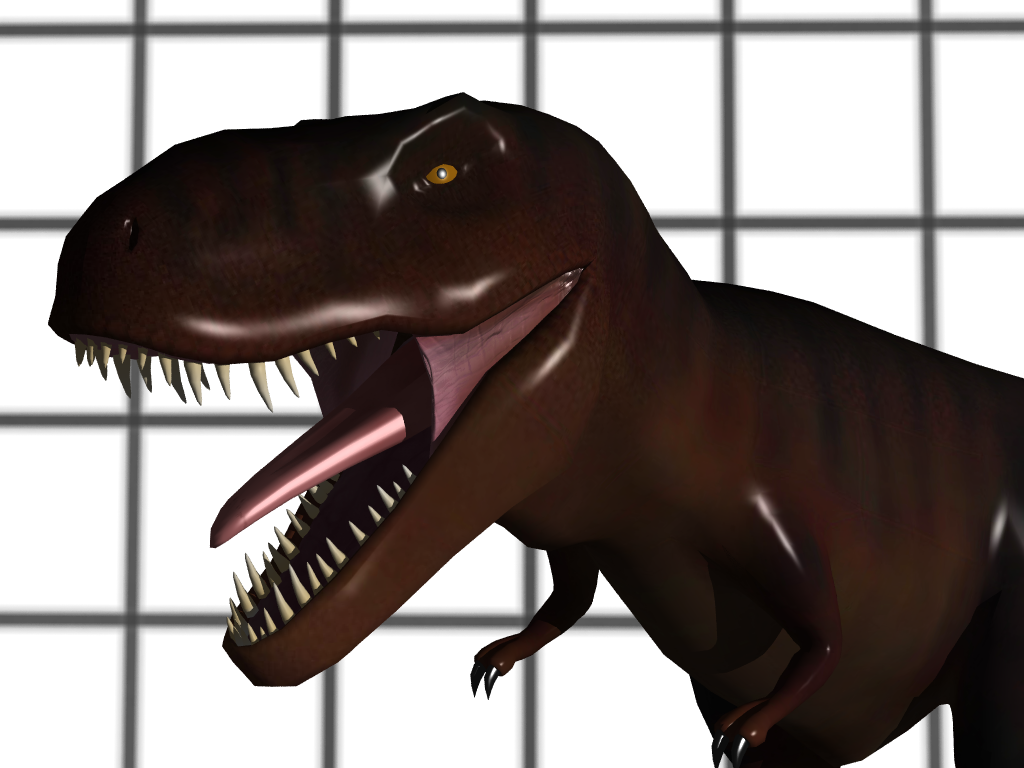
\includegraphics[width=\textwidth]{./img/texturierung/trex_without_normalmap}
   \captionof{figure}{Das Modell eines T-Rex ohne "`Normal Mapping"': Laufzeit 2,08 Sekunden}
   \label{fig:trex_without_normalmap}
\end{minipage}
   \hfill
\begin{minipage}[t]{0.45\textwidth}
   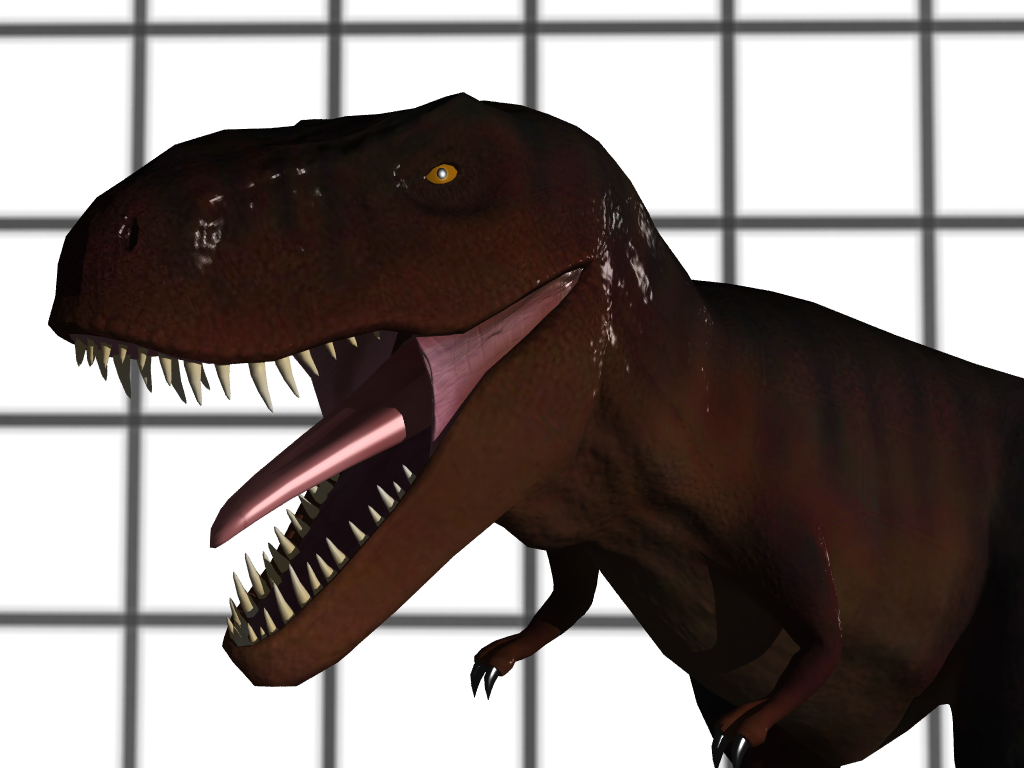
\includegraphics[width=\textwidth]{./img/texturierung/trex_with_normalmap}
   \captionof{figure}{Das selbe Modell mit "`Normal Mapping"': Laufzeit 2,1 Sekunden}
   \label{fig:trex_with_normalmap}
\end{minipage}

%\begin{figure}[t]
%    \centering
%    \begin{minipage}[b]{1.0\textwidth}
%        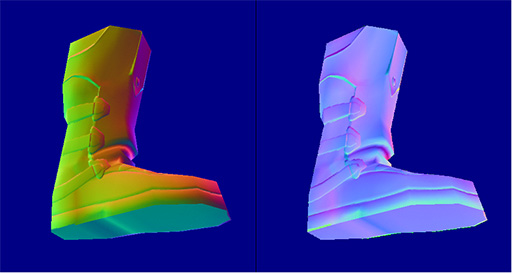
\includegraphics[width=\textwidth]{./img/texturierung/normalmaps}
%        \caption{Links: Regenbogenfarbene Objektraum-"'Normal Map"'. Rechts: Blaue Tangentialraum-"'Normal Map"'.\protect\footnotemark}
%        \label{Bild}
%    \end{minipage}
%\end{figure}

\begin{center}
    \begin{minipage}[t]{0.35\textwidth}
        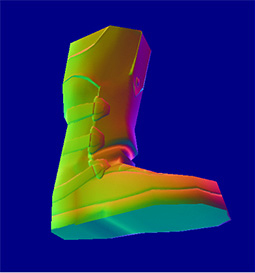
\includegraphics[width=\textwidth]{./img/texturierung/objektraum}
        \captionof{figure}{Objektraum-"'Normal Map"'\protect\footnotemark}
        \label{fig:objektraum}
    \end{minipage}
       \hspace{0.75cm}
       \addtocounter{footnote}{-1}\addtocounter{Hfootnote}{-1} % Setzt den Counter von footnotemark um 1 herunter
    \begin{minipage}[t]{0.35\textwidth}
       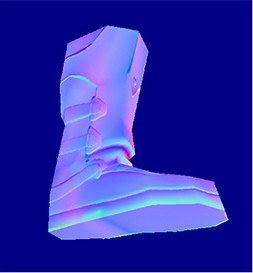
\includegraphics[width=\textwidth]{./img/texturierung/tangentialraum}
       \captionof{figure}{Tangentialraum-"'Normal Map"'\protect\footnotemark}
       \label{fig:tangentialraum}
   \end{minipage}
\end{center}
   
\footnotetext{Quelle: http://docs.cryengine.com/display/SDKDOC4/Tangent+Space+Normal+Mapping}

Man unterscheidet zwei Arten von "`Normal Maps"', die eine bezieht sich auf den Objektraum und die andere auf den Tangentialraum der Geometrie. In Abb.~\ref{fig:objektraum} sieht man, dass die Objektraum-"'Normal Map"' regenbogenfarben ausfällt. Dies liegt daran, dass die Objektraum-"'Normal Map"' Vektoren speichert, die direkt als Normalen an einem Oberflächenschnittpunkt benutzt werden können, solange das zugrunde liegende Objekt untransformiert bleibt. Gerade für geschlossene Polygonnetze entspricht das einer Verteilung der Normalen auf der Oberfläche einer Kugel, weshalb viele unterschiedliche Farben in der Textur zum Vorschein kommen.


Um nun für eine Objektraum-"'Normal Map"' die Normale an einem Schnittpunkt zu erhalten, sucht man den zum Schnittpunkt passenden Texel wie im vorherigen Abschnitt beschrieben. Die einzelnen Bytes des im Texel gespeicherten RBG-Werts sind dann \( r_{RGB} \) für Rot, \( g_{RGB} \) für Grün und \( b_{RGB} \) für Blau, wobei jede Komponente maximal den Wert 255 annehmen kann. Die Komponenten \( {n'}.x, {n'}.y \text{ und } {n'}.z \) der neuen variierten Normalen \( \boldsymbol{n'} \) ergeben sich dann durch:

\begin{equation}
    n'.x = \frac{2 \cdot r_{RGB} - r_{RGB}}{255}; \quad n'.y = \frac{2 \cdot g_{RGB} - g_{RGB}}{255}; \quad
    n'.z = \frac{2 \cdot b_{RGB} - b_{RGB}}{255}; \label{eq:texel_vektor}
\end{equation}

Wird das Objekt durch Transformationsmatrix \( \boldsymbol{T} \) transformiert, so muss die aus der Objektraum-"`Normal Map"' erhaltene Normale mit \( \boldsymbol{(T^{-1})}^\intercal \) transformiert werden.


Eine Tangentialraum-"'Normal Map"' (Abb.~\ref{fig:tangentialraum} ) bezieht sich hingegen auf die Koordinatenbasis, die durch einen Vektor senkrecht zur Oberfläche und zwei Tangentialvektoren gegeben ist. Der Ursprung der Basis befindet sich am Strahl-Objekt Schnittpunkt. Da auch bei unebenen Oberflächen die meisten Normalen relativ senkrecht auf der Oberfläche stehen und der Blauanteil der Textur für diese senkrechte (z-) Komponente verantwortlich ist, erscheint die Textur überwiegend bläulich.

Die Konstruktion der Koordinatenbasis beginnt mit der Festlegung der z-Achse. Dafür kann die beim Schnitttest berechnete Normale verwendet werden. Es ist jedoch auch möglich, eine interpolierte Normale zu benutzen, wie sie bei der glatten Schattierung verwendet wird, wodurch man harte Übergänge vermeidet.
Prinzipiell gibt es für die x- und y-Achse, die durch Tangentialvektoren festgelegt werden, beliebig viele Orientierungen, solange alle 3 Vektoren orthogonal zueinander stehen. Denn jede Drehung der x- und y-Achse um die z-Achse erzeugt weiterhin eine korrekte Koordinatenbasis im Tangentialraum. Für eine konsistente Schattierung ist es jedoch erforderlich, die Tangentialvektoren entlang der uv-Koordinaten auszurichten. Im Fall von triangulierten Objekten betrachtet man, wie sich die uv-Koordinaten entlang der Dreieckskanten verändern, indem man die Differenzen 
\( \Delta \boldsymbol{uv_0} = \boldsymbol{uv_1} - \boldsymbol{uv_0 }\) und \( \Delta \boldsymbol{uv_1} = \boldsymbol{uv_2} - \boldsymbol{uv_0} \) (vgl. Abb.\ref{fig:textur} ) bildet. Ebenso erzeugt man die Dreieckskanten \( \boldsymbol{e_0} = \boldsymbol{p_1} - \boldsymbol{p_0} \) und \( \boldsymbol{e_1} = \boldsymbol{p_2} - \boldsymbol{p_0} \), wobei  sich die uv-Koordinate \( \boldsymbol{uv_0} \) am Punkt \( \boldsymbol{p_0} \), \( \boldsymbol{uv_1} \) am Punkt \( \boldsymbol{p_1} \) usw. befindet.
Anhand der Komponenten von \( \Delta \boldsymbol{uv_0} \) und \( \Delta \boldsymbol{uv_1} \) wird eine Linearkombination mit den benötigten Basisvektoren d.h. mit der Tangenten \( \boldsymbol{t} \) und mit der Bitangenten \( \boldsymbol{b} \) gesucht, die den Kanten \( \boldsymbol{e_0} \) und \( \boldsymbol{e_1} \) entspricht \cite{openglnormal}:

\begin{align*}
    \boldsymbol{e_0} = {\Delta \boldsymbol{uv_0}.u } \cdot \boldsymbol{t} + {\Delta \boldsymbol{uv_0}.v } \cdot \boldsymbol{b} \\
    \boldsymbol{e_1} = {\Delta \boldsymbol{uv_1}.u } \cdot \boldsymbol{t} + {\Delta \boldsymbol{uv_1}.v } \cdot \boldsymbol{b}
\end{align*}

wobei \( {\Delta \boldsymbol{uv_0}.u } \) die \( u \)-Komponente von \( \Delta \boldsymbol{uv_0} \),  \( {\Delta \boldsymbol{uv_0}.v } \) die \( v \)-Komponente von \( \Delta \boldsymbol{uv_0} \) usw. ist.
Anhand dieses Gleichungssystems lässt sich nun \( \boldsymbol{t} \) und \( \boldsymbol{b} \) bestimmen, durch:

\begin{align*}
    r =& ({\Delta \boldsymbol{uv_0}.u } \cdot {\Delta \boldsymbol{uv_1}.v } - {\Delta \boldsymbol{uv_0}.v } \cdot {\Delta \boldsymbol{uv_1}.u } )^{-1} \\
    \boldsymbol{t} =& ( \boldsymbol{e_0} \cdot {\Delta \boldsymbol{uv_1}.v } - \boldsymbol{e_1} \cdot {\Delta \boldsymbol{uv_0}.v } ) \cdot r \\
    \boldsymbol{b} =& ( \boldsymbol{e_1} \cdot {\Delta \boldsymbol{uv_0}.u } - \boldsymbol{e_0} \cdot {\Delta \boldsymbol{uv_1}.u } ) \cdot r
\end{align*}

Die Vektoren \( \boldsymbol{t}, \boldsymbol{b} \text{ und } \boldsymbol{n} \) sind zwar linear unabhängig bilden jedoch keine ONB, weshalb das Gram-Schmidtsches Orthogonalisierungsverfahren eingesetzt wird, um diese Eigenschaft herzustellen. Zu beachten ist, dass dabei die Richtung von \( \boldsymbol{n} \) unverändert bleibt. Im Kontext des Verfahrens von Gram-Schmidt bedeutet das, dass man den Algorithmus mit dem Vektor \( \boldsymbol{n} \) beginnt.

Wie bei der Objektraum-"'Normal Map"' wird nun der zum Strahl-Objekt Schnittpunkt passende Texel gesucht und ein Vektor \( \boldsymbol{m} \)
gemäß der Gleichungen~\ref{eq:texel_vektor} erzeugt. Jedoch ist dies noch nicht die endgültige Normale \( \boldsymbol{n'} \). Diese erhält man durch:

\begin{equation*}
    \boldsymbol{n'} = \boldsymbol{t} \cdot {\boldsymbol{m}.x } + \boldsymbol{b} \cdot {\boldsymbol{m}.y } + \boldsymbol{n} \cdot  {\boldsymbol{m}.z }
\end{equation*}

wobei \( {\boldsymbol{m}.x }, {\boldsymbol{m}.y } \text{ und }  {\boldsymbol{m}.z } \) die x, y und z-Komponenten des Vektors \( \boldsymbol{m} \) sind.








\chapter{Bildkorrektur}

Ein bekanntes Problem der Computergrafik sind die Alias-Effekte. Zu den bekanntesten gehört die Treppenbildung an nahezu horizontal bzw. vertikal verlaufenden Kanten, oder der Moiré-Effekt bei dem z.B. durch Überlagerung zweier feiner Gitter ein gröberes Muster entsteht.
Beispiele hierfür liefert Abb. \ref{fig:midpoint}. So kann an den horizontal verlaufenden Linien des Schachbretts Treppenbildung beobachtet werde. Ebenso zeigt sich eine Form des Moiré-Effekt und zwar in den hinteren Reihen des Schachbretts, in denen Kacheln wieder größer werden.

Eine Erklärung für diese Erscheinungen findet man in der Signalverarbeitung. Dort tritt "`Aliasing"' auf, wenn das ursprüngliche Signal nicht mit einer ausreichend hohen Frequenz abgetastet wird, und deshalb nicht vollständig rekonstruiert werden kann. Um ein Signal fehlerfrei rekonstruieren zu können muss die Abtastfrequenz mindestens doppelt so hoch sein, wie die höchsten Frequenzanteile des Signals. Die Grenzfrequenz ab der eine fehlerfreie Rekonstruktion möglich ist, heißt Nyquist-Frequenz.

Im Kontext des "`Raytracing"' ist das Ursprungssignal eine kontinuierliche Funktion über,  auf den Sensor einfallender, Strahldichten. Dieses Signal wird an diskreten Punkten abgetastet. Bisher geschah dies, indem Strahlen durch den Mittelpunkt eines PEE geschossen wurden.
Zur Bildkorrektur schießt man durch ein einzelnes PEE mehrere Strahlen, um so die Abtastfrequenz zu erhöhen und das Ursprungssignal so gut wie möglich rekonstruieren zu können.

% Die Stellen an denen das PEE vom Strahl durchdrungen werden "`Samples"' genannt und das Verfahren zur Erzeugung der "`Samples"' als "`Sampling"' bezeichnet.


\section{Erzeugung geeigneter Abtastpunkte}

Das Verfahren zur Erzeugung weiterer Abtastpunkte auf den PEE wird auch als "`Sampling"' bezeichnet. Bevor die einzelnen "`Sampling"'-Verfahren vorgestellt werden, werden informell Sachverhalte aus der Signalverarbeitung erläutert, um besser nachvollziehen zu können, was beim "`Sampling"' beachtet werden sollte.

Multidimensionale Signale zeigen eine räumliche Änderung, wie z.B. die Verteilung der Strahldichten über die Projektionsebene. Solche Signale lassen sich als Funktionen im Ortsraum darstellen. Durch die Fourier-Transformation lassen sich Signale vom Ortsraum in den Frequenzraum transformieren. Hier wird sichtbar wie viele Anteile des Signals in einem bestimmten Frequenzband liegen. Das Signal dargestellt als Funktion wird abgetastet, indem die Funktion mit einem Dirac-Kamm multipliziert wird. Der Dirac-Kamm besteht aus einer Folge von Dirac-Stößen, die sich nach konstanten Perioden \( T \) der Abtastfrequenz wiederholen. Die Periode \( T \) hängt von der Anzahl der Abtastpunkten - den "`Samples"' - ab. Je mehr Abtastpunkte vorhanden sind desto kleiner ist \( T \). Dieser Prozess der Signalabtastung kann auch im Frequenzbereich beobachtet werden. Nur handelt es sich hier um eine Faltung des Frequenzspektrums mit einem Dirac-Kamm der Periode \( \frac{1}{T} \). Sind nicht genug Abtastpunkte vorhanden, überlagern sich Frequenzbereiche des Signals. Diese Überlagerungen im Frequenzraum lassen sich nicht mehr fehlerfrei rekonstruieren.

Zwei Dinge versucht man deshalb bei den "`Sampling"'-Verfahren zu erreichen.
Einerseits kann das Überlappen von Frequenzbereichen im Frequenzraum reduziert werden, indem man mehr Strahlen durch ein PEE schießt und so die Anzahl an Abtastpunkten erhöht, denn dies vergrößert die Abstände der Dirac-Stöße im Frequenzraum. Dennoch ist es möglich, dass sich Überlappungen nicht komplett verhindern lassen, weil dazu zu viele "`Samples"' benötigt werden, was sich linear in der Laufzeit niederschlägt. In diesem Fall versucht man die Regelmäßigkeit, mit der Abtastpunkt auf Abtastpunkt folgt, zu stören. Denn diese Regelmäßigkeit verursacht die störenden Alias-Effekte und Bildartefakte. Ziel ist es daher das PEE möglichst mit geringer Diskrepanz (das heißt die "`Samples"' sollten einen möglichst großen Abstand zueinander haben) jedoch nicht regelmäßig durch "`Samples"' aufzuteilen. Dadurch werden Alias-Effekte und Bildartefakte durch Rauschen ersetzt, was für den Betrachter natürlicher wirkt.

\begin{itemize}
    \item Mittelpunkt "`Sampling"': Die einfachste Art des "`Sampling"', indem durch den Mittelpunkt eines PEE ein Primärstrahl geschossen wird. Abb.~\ref{fig:midpoint} zeigt durch die geringe und regelmäßige Abtastung Treppenbildung an Kanten und Schatten des Buddhas, sowie horizontal und vertikal verlaufenden Kanten der Kacheln. Nahe des Horizonts kommt es zu Bildartefakte durch wieder größer werdende Kacheln.
    
    \item "`Random Sampling"': Die Komponenten eines "`Samples"' werden gleichverteilt entlang der x-und y-Achse des PEE gezogen. Abb.~\ref{fig:random4} zeigt den Ausschnitt mit 4 "`Samples"'. Durch das komplett zufällige ziehen der "`Samples"', kann es zu schlechten Verteilungen durch Pulk Bildung kommen. Zwar wurde die Treppenbildung entfernt, dafür erscheinen Kanten und Schatten ausgefranst. Die hinteren Bildartefakte wurden durch Rauschen ersetzt.
    
    \item "`Stratified Sampling"': Das PEE wird in kleinere gleichgroße Quadrate unterteilt. Innerhalb dieser Quadrate wird je ein "`Sample"' durch "`Random Sampling"' erzeugt. Abb.~\ref{fig:stratified4} zeig den Ausschnitt mit 4 "`Samples"'. Der Ausschnitt ähnelt sehr dem des "`Random Sampling"', jedoch mit weniger Rauschen, da durch die weitere Aufteilung des PEE die Pulk-Bildung verhindert wird.
    
    \item "`Hammersley Sampling"': Aus \( n \) zu erzeugenden "`Samples"' berechnet sich die erste Komponente des \( i \)-ten "`Samples"' aus \( \frac{i}{n} \) und die zweite aus dem \( i \)-ten Element der "`Van der Corput"' Zahlenreihe zur Basis 2. Abb.~\ref{fig:hammersley4} zeigt bei 4 "`Samples"' bessere Glättung der Kanten als "`Random"' oder "`Stratified"' Sampling, da kein ausfransen zu erkennen ist. Es zeichnet sich durch geringe Diskrepanz und unregelmäßiger Verteilung der "`Samples"' aus. Jedoch fehlt der Zufallsfaktor bei diesem Verfahren, was neue Alias-Effekte anstelle von Rauschen ins Bild einbringt. Dies wird durch 2 graue Streifen in der Nähe des Horizonts deutlich.
    
   
\end{itemize}


\newpage

\begin{center}
\begin{minipage}[t]{0.72\textwidth}
    \centering
    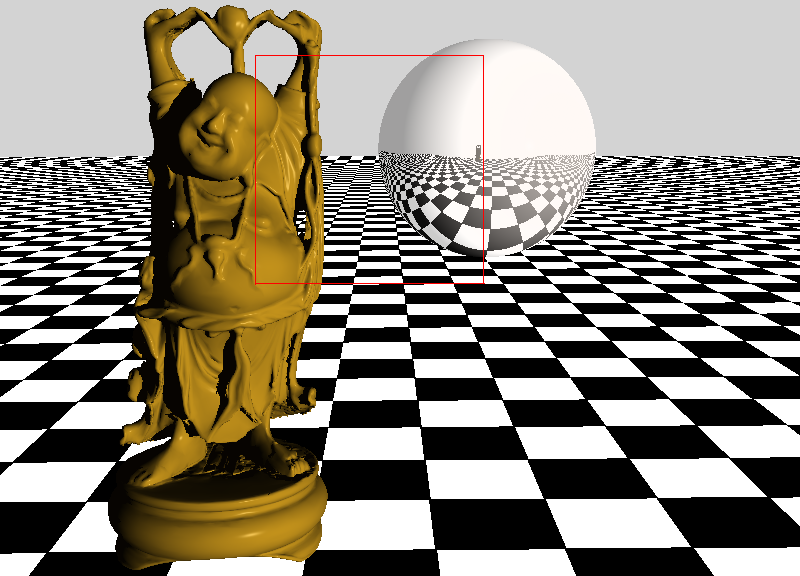
\includegraphics[width=\textwidth]{./img/bildkorrektur/midpoint_ganz.png}
    \captionof{figure}{Komplette Szene "`gerendert"' mit Mittelpunkt "`Sampling"'. Die folgenden Ausschnitte verwenden unterschiedliche "`Sampling"' Verfahren. Die Zahl steht für die Anzahl verwendeter "`Samples"'.}
    \label{fig:midpoint_ganz}
\end{minipage}
\end{center}
\begin{minipage}[t]{0.33\textwidth}
    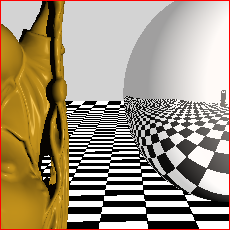
\includegraphics[width=\textwidth]{./img/bildkorrektur/midpoint.png}
    \captionof{figure}{1 Mittelpunkt}
    \label{fig:midpoint}
\end{minipage}
\begin{minipage}[t]{0.33\textwidth}
    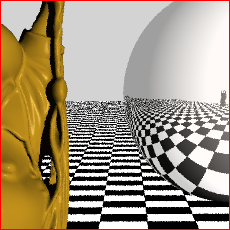
\includegraphics[width=\textwidth]{./img/bildkorrektur/random4.png}
    \captionof{figure}{4 "'Random"'}
    \label{fig:random4}
\end{minipage}
\begin{minipage}[t]{0.33\textwidth}
    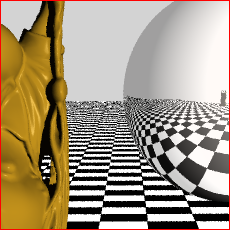
\includegraphics[width=\textwidth]{./img/bildkorrektur/stratified4.png}
    \captionof{figure}{4 "'Stratified"'}
    \label{fig:stratified4}
\end{minipage}\\
\begin{minipage}[t]{0.33\textwidth}
    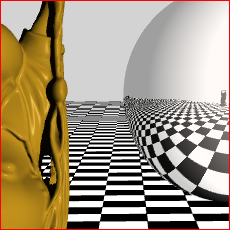
\includegraphics[width=\textwidth]{./img/bildkorrektur/hammersley4.png}
    \captionof{figure}{4 "'Hammersley"'}
    \label{fig:hammersley4}
\end{minipage}
\begin{minipage}[t]{0.33\textwidth}
    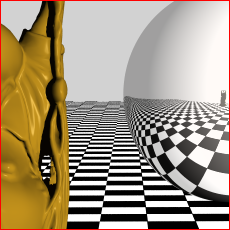
\includegraphics[width=\textwidth]{./img/bildkorrektur/stratified64.png}
    \captionof{figure}{64 "`Stratified"'}
    \label{fig:stratified64}
\end{minipage}
\begin{minipage}[t]{0.33\textwidth}
    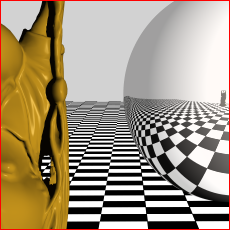
\includegraphics[width=\textwidth]{./img/bildkorrektur/hammersley64.png}
    \captionof{figure}{64 "`Hammersley"'}
    \label{fig:hammersley64}
\end{minipage}

\FloatBarrier

\chapter{Galerie}



\begin{figure}[ht]
    \centering
    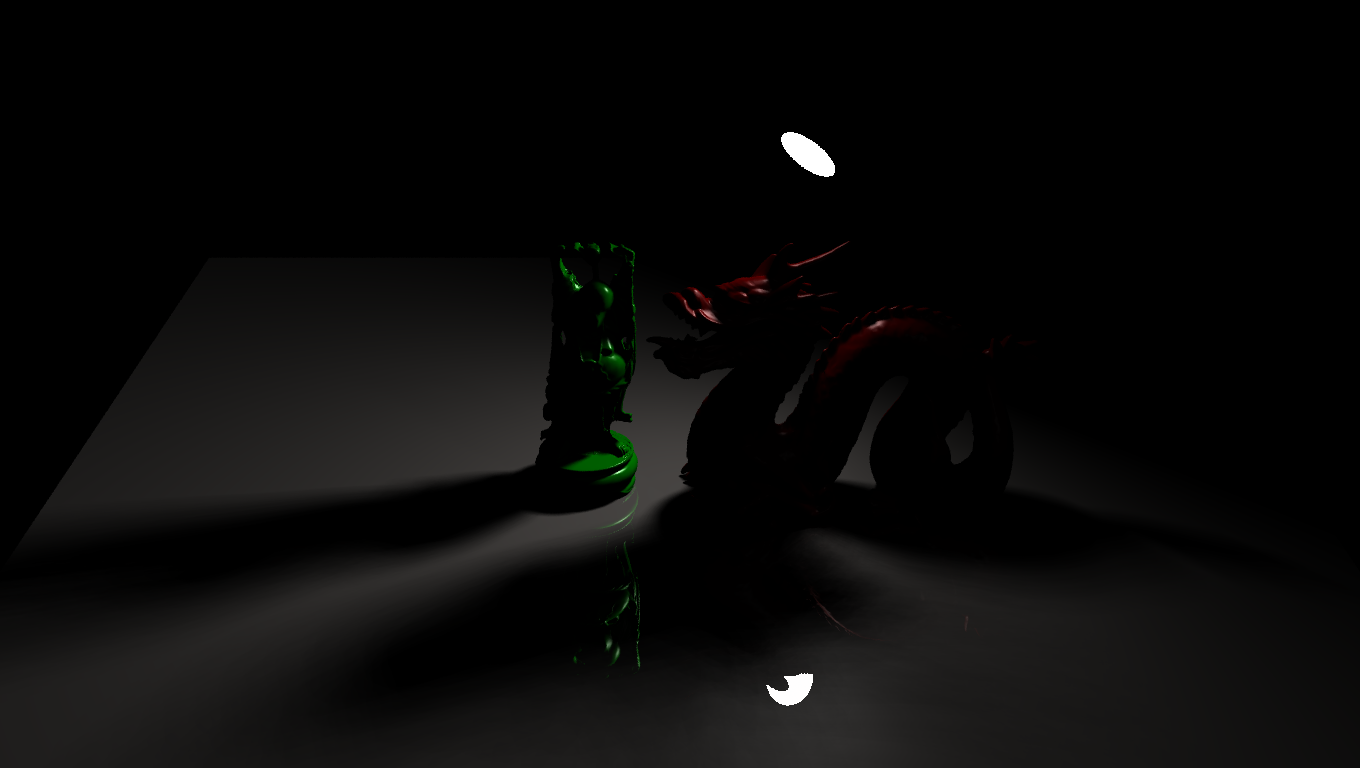
\includegraphics[width=1\textwidth]{./img/galerie/bhudda_dragon_glossy_plane_dark}
    \caption{Phong schattierter "`Stanford Buddha"' und "`Stanford Dragon"' auf spiegelndem Untergrund. Die Szene wird von zwei runden Flächenlichter beleuchtet.}
    \label{fig:bhudda_dragon_plane_glossy_dark}
\end{figure}



\begin{figure}[ht]
    \centering
    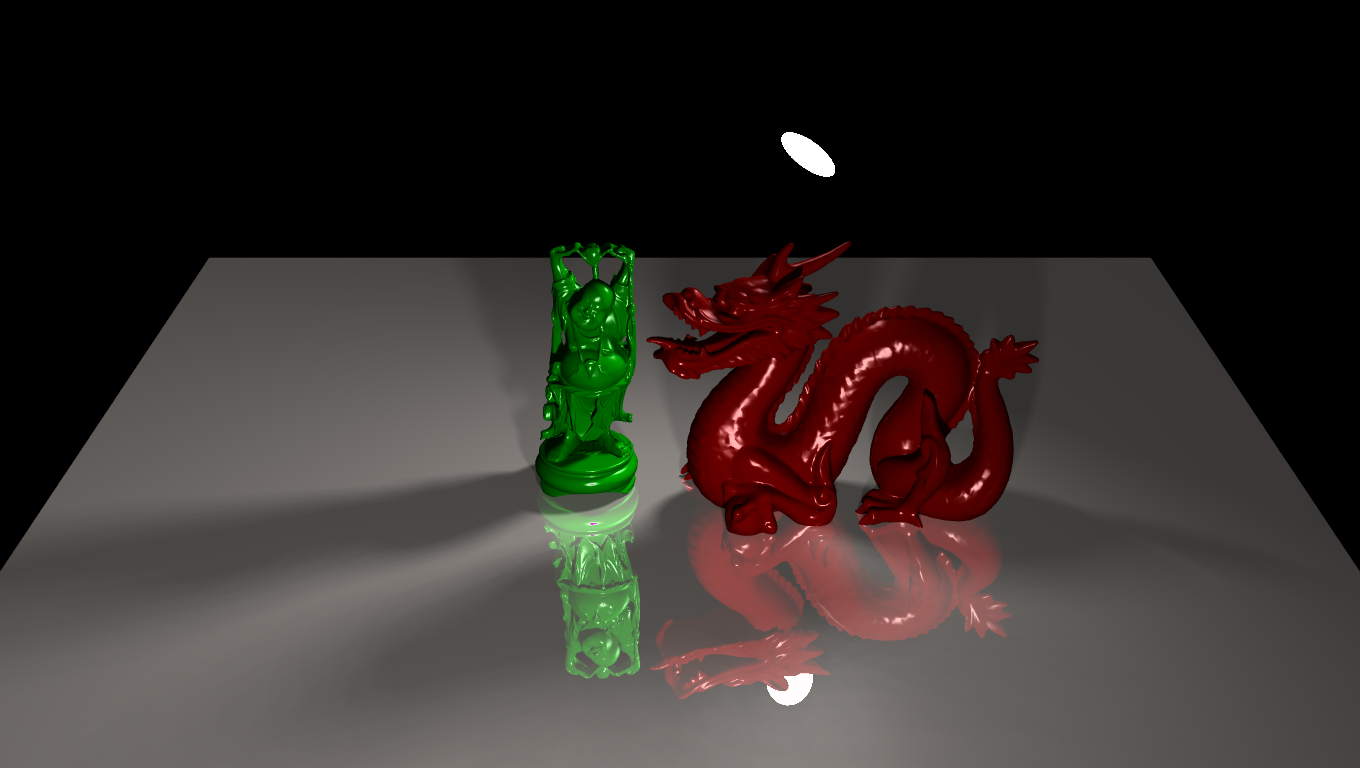
\includegraphics[width=1\textwidth]{./img/galerie/bhudda_dragon_glossy_plane_bright}
    \caption{Phong schattierter "`Stanford Buddha"' und "`Stanford Dragon"' auf spiegelndem Untergrund. Die Szene wird von zwei runden Flächenlichter beleuchtet.}
    \label{fig:bhudda_dragon_plane_glossy_bright}
\end{figure}



\begin{figure}[ht]
    \centering
    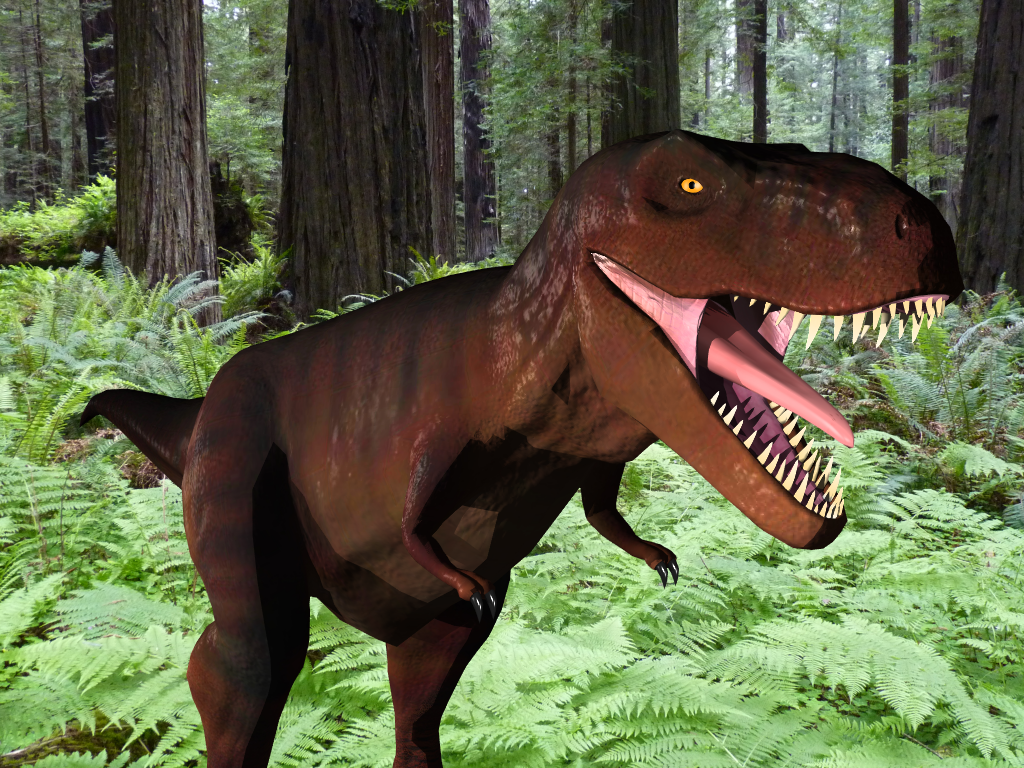
\includegraphics[width=1\textwidth]{./img/galerie/t-rex}
    \caption{Texturiertes Modell eines T-Rex, bestehend aus Bildtextur und "`Normal Map"'.}
    \label{fig:t-rex}
\end{figure}


\begin{figure}[ht]
    \centering
    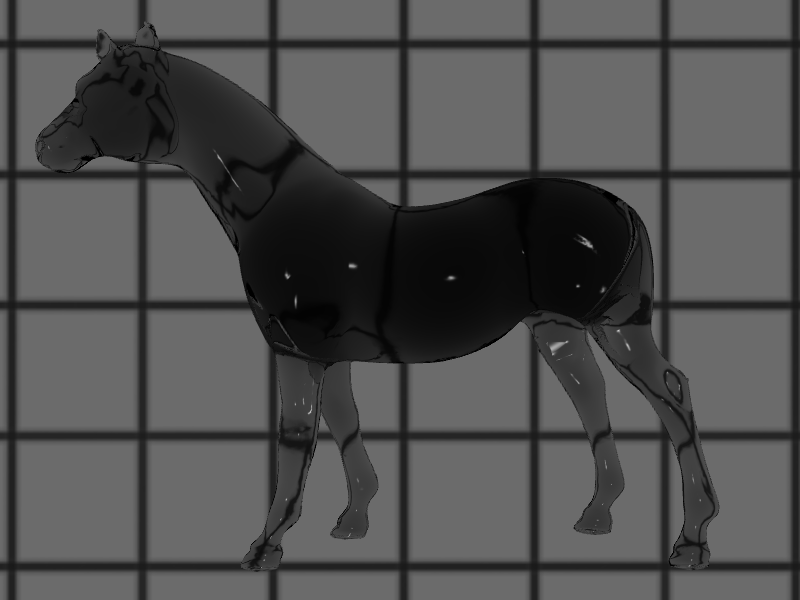
\includegraphics[width=1\textwidth]{./img/galerie/pferd_trans_dir.png}
    \caption{Pferdemodell gerendert mit dielektrischem Material unter Verwendung eines Brechungsindex von 1,3 und direktionalem Licht. Das Licht wird im Bauch des Pferdes stärker absorbiert als in den dünnen Beinen, wodurch diese dunkler wirkt.}
\end{figure}


\begin{figure}[ht]
    \centering
    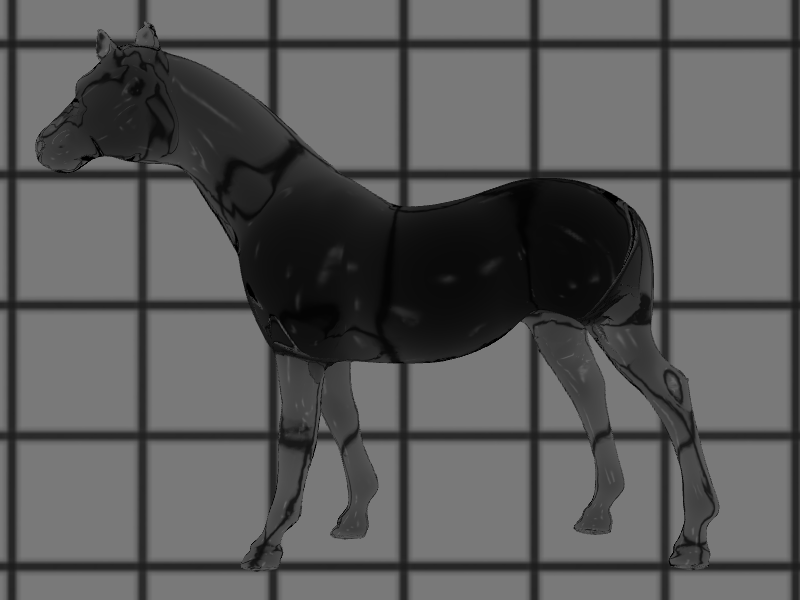
\includegraphics[width=1\textwidth]{./img/galerie/pferd_trans_flaeche.png}
    \caption{Pferdemodell gerendert mit dielektrischem Material unter Verwendung eines Brechungsindex von 1,3 und Flächenlicht. Das Licht wird im Bauch des Pferdes stärker absorbiert als in den dünnen Beinen, wodurch diese dunkler wirkt.}
\end{figure}

\begin{figure}[ht]
    \centering
    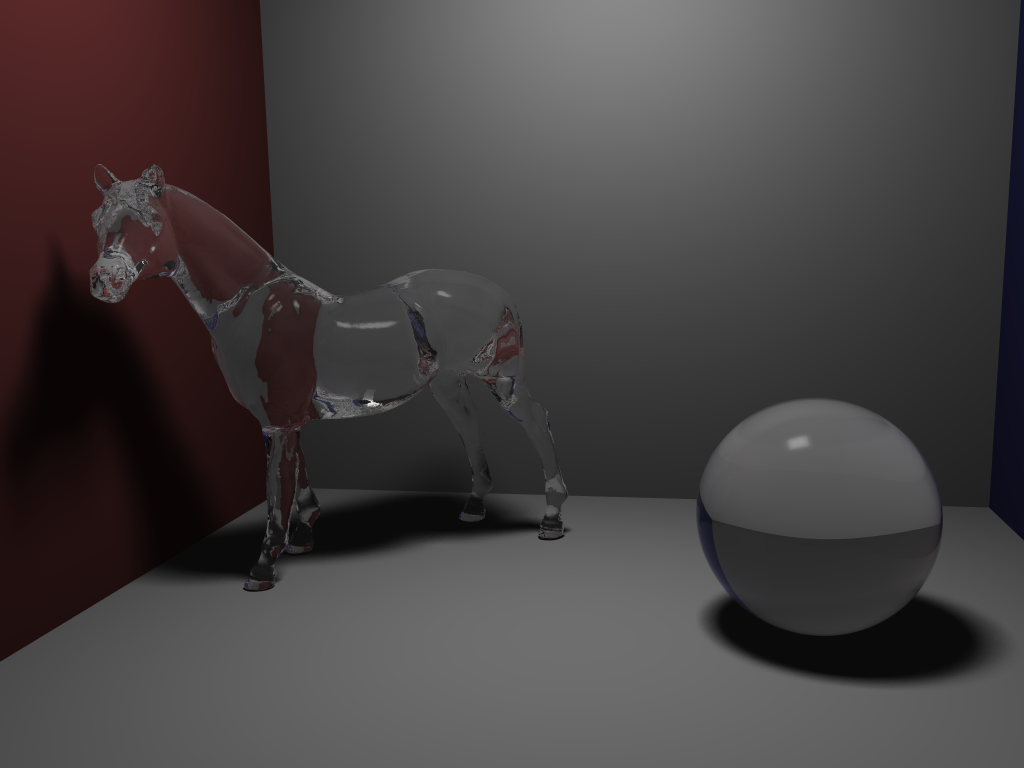
\includegraphics[width=1\textwidth]{./img/schattierung/dielectric_1_1,3.png}
    \caption{Pferdemodell und Kugel in "`Cornell box"'. Gerendert mit dielektrischem Material unter Verwendung eines Brechungsindex von 1,35 und Flächenlicht.}
\end{figure}

\begin{figure}[ht]
    \centering
    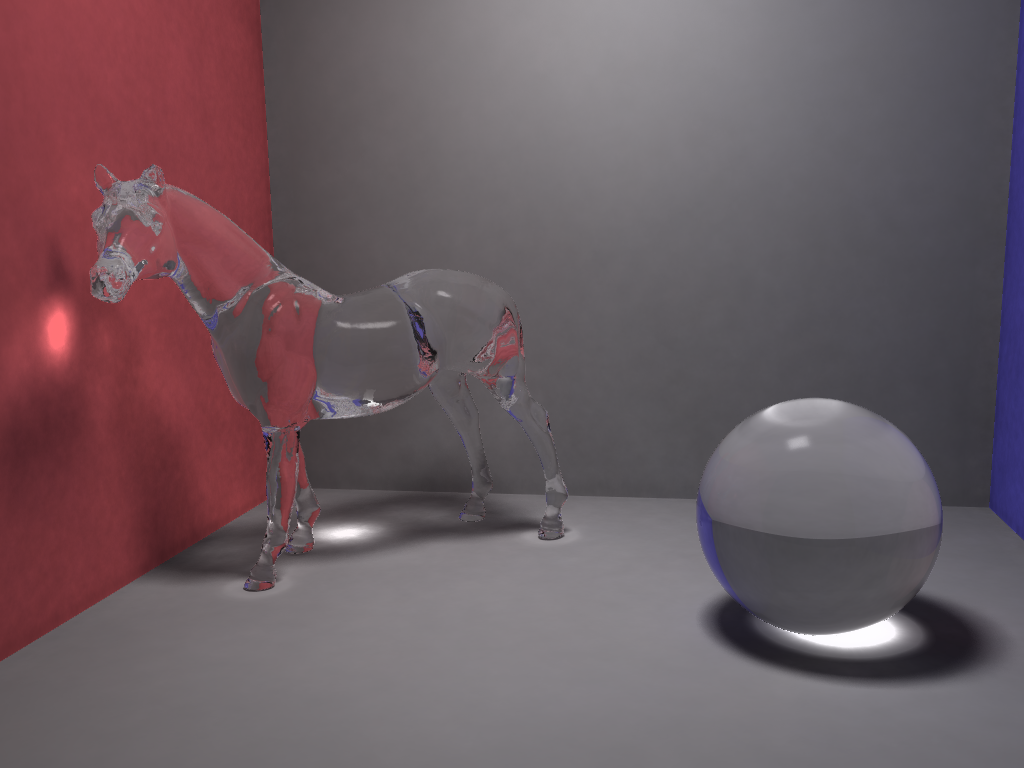
\includegraphics[width=1\textwidth]{./img/schattierung/dielectric_photon.png}
    \caption{Pferdemodell und Kugel in "`Cornell box"'. Gerendert mit dielektrischem Material unter Verwendung eines Brechungsindex von 1,35 und Flächenlicht. Verwendung von "`Photon Mapping"' mit 5 Millionen Photonen, zur Darstellung von Kaustiken und indirekter Beleuchtung. Zur Berechnung der Bestrahlungsstärke wurde eine konvexe Hülle verwendet, um dunkle Kanten und Ecken zu vermeiden.}
\end{figure}


\begin{figure}[ht]
    \centering
    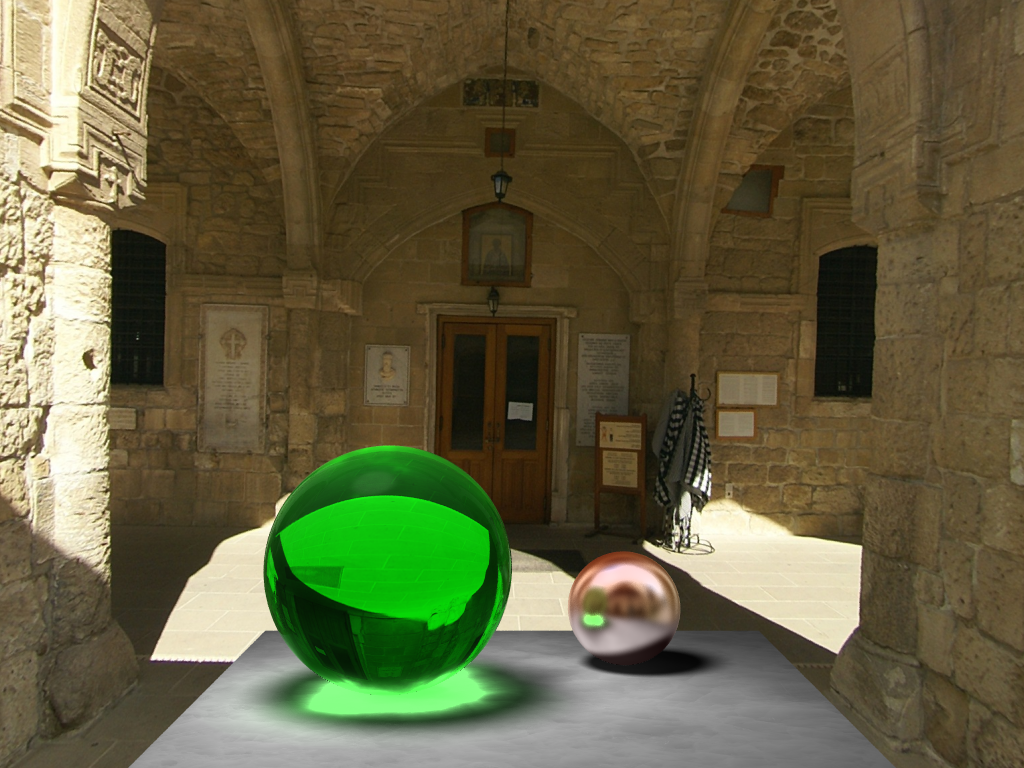
\includegraphics[width=1\textwidth]{./img/galerie/sphere_skybox_photon_clear}
    \caption{Transparente und matt spiegelnde Kugel in einer Skybox der Lazarus-Kirche. "`Photon Mapping"' erzeugt Kaustiken.}
    \label{fig:sphere_skybox_photon_clear}
\end{figure}



\begin{figure}[ht]
    \centering
    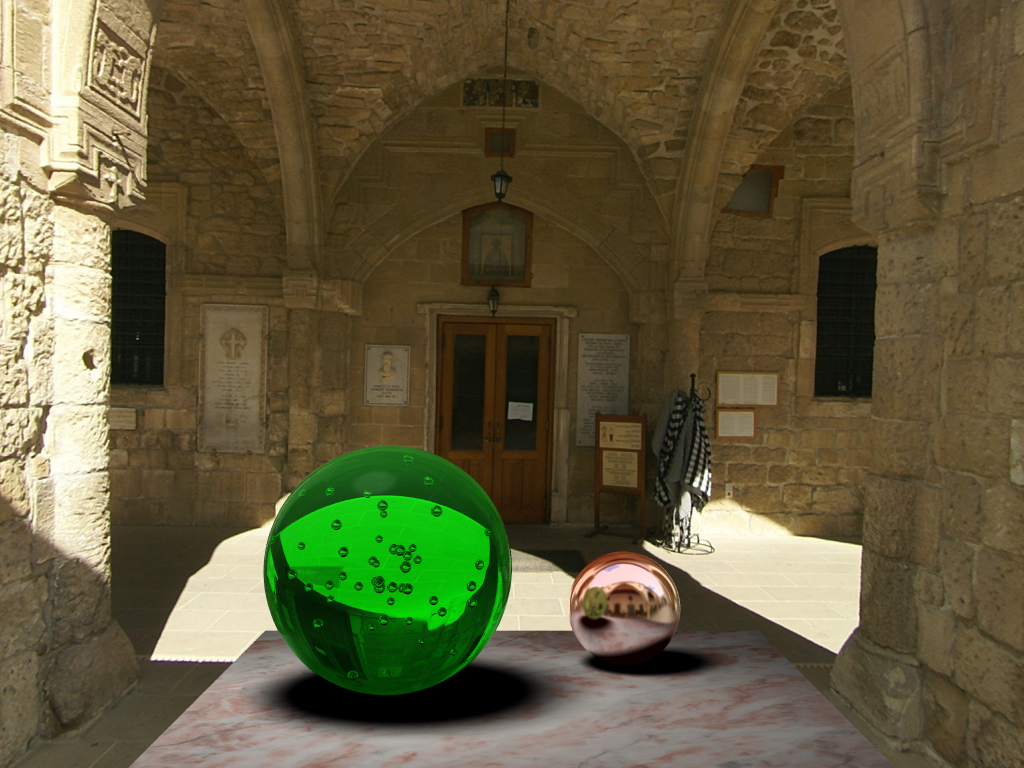
\includegraphics[width=1\textwidth]{./img/galerie/sphere_skybox_without_photon}
    \caption{Transparente Kugel mit eingeschlossen Luftblasen und spiegelnde Kugel in einer Skybox der Lazarus-Kirche.}
    \label{fig:sphere_skybox_photon_without_photon}
\end{figure}



\begin{figure}[ht]
    \centering
    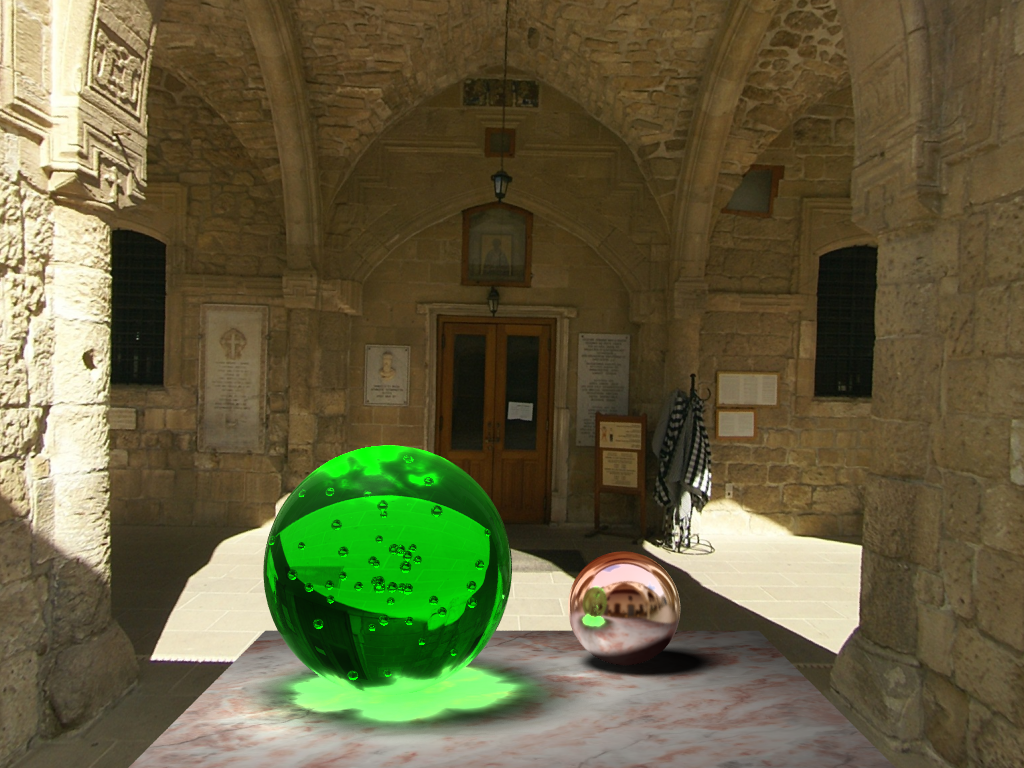
\includegraphics[width=1\textwidth]{./img/galerie/sphere_skybox_with_photon}
    \caption{Transparente Kugel mit eingeschlossen Luftblasen und spiegelnde Kugel in einer Skybox der Lazarus-Kirche. "`Photon Mapping"' sorgt für Kaustiken.}
    \label{fig:sphere_skybox_with_photon}
\end{figure}

%\include{zielsetzung.tex}
%\section{Szenegenerierung- und Darstellung}

Bevor der eigentliche Render-Vorgang beginnen kann muss man eine Szene erzeugen und diese in eine, für den Raytracer verwendbare interne Repräsentation bringen. Dabei kann die Beschreibung einer Szene sehr komplex werden. Einerseits durch die geometrische Darstellung der Objekte(Objekte mit mehreren Tausend "`vertices"') aber auch durch ihre Eigenschaften. Gegeben z.B. durch Normalenvektoren, Materialeigenschaften, Texturkoordinaten, Art der Lichtquelle, Sichtfeld der Kamera usw.\\


Um die Möglichkeit offen zu halten später eine eigene "`scene description language"' zu definieren und zu verwenden wird der Raytracer um eine einfache Parser-Klasse erweitert, die dies gewährleisten soll. Für den Anfang reicht es die einzelnen Instanzen der benötigten Objekte direkt im Code zu erzeugen. Jedoch wäre es im späteren Verlauf des Projekts denkbar auch komplexere triangulierte Objekte zu verwenden, die sich eben nicht mehr so einfach per Code beschreiben lassen. Ein Ausweg aus dieser Problematik könnte z.B das von "`Wavefront"' entwickelte "`obj."'-Dateiformat bieten. Da es von vielen 3D-Modellierungsprogrammen 
unterstützt wird können dort Objekte modelliert werden und dann auf einfache Art und Weise dem Raytracer zur Verfügung gestellt werden. 
%\section{Programmablauf}

In diesem Kapitel soll eine Übersicht über den Ablauf des Programms verschafft werden. Der grobe Ablauf, vom Start des Programms bis zur Erzeugung des eigentlichen Bildes lässt sich aus Abbildung~\ref{fig_Programmablaufplan} entnehmen. Im Text werden dann die einzelnen Bereiche der Abbildung detaillierter erläutert.\\

Der Raytracer wird über eine Kommandozeile oder aus einer IDE wie "`Microsoft Visual Studio"' gestartet. Dabei können dem Programm die Optionen aus Tabelle~\ref{tab_Optionen} mitgegeben werden. Wenn keine Optionen angegeben werden benutzt der Raytracer die Standardkonfiguration.


%%%%%%%%%%%%%%%%%%%%%%%%%%%%%%%%Tabelle%%%%%%%%%%%%%%%%%%%%%%%%%%%%%%%%%%%%%%%%%%%%%%%%%%%%%%%%%%%%%%%
\begin{table}[h]
    \begin{tabular}{|c|c|p{8cm}|}
    \hline 
    \textbf{Argument} & \textbf{Standardwert} & \textbf{Bedeutung} \\ 
    \hline 
    $--$ncores $<$int$>$ & 1 & Legt die Anzahl der Verwendeten Threads fest (sollte der Anzahl 
    an CPU-    Cores entsprechen) \\ 
    \hline 
     $--$outfile $<$string$>$ & "`out.ppm"' & Legt Ausgabeverzeichnis und Name des gerenderten 
     Bildes fest     \\ 
    \hline 
    $--$verbose $<$int$>$ & 1 & Legt das Ausgabe-Level des Logger fest \\ 
    \hline 
    $--$window $<$bool$>$ & false & Zeige das Bild direkt nach dem Rendern in einem externen Fenster \\ 
    \hline 
    $--$help & $-$ & Zeigt den Hilfetext an \\
    \hline
    \end{tabular}
    \caption{Kommandozeilenoptionen}
    \label{tab_Optionen}
\end{table}
%%%%%%%%%%%%%%%%%%%%%%%%%%%%%%%%%%%%%%%%%%%%%%%%%%%%%%%%%%%%%%%%%%%%%%%%%%%%%%%%%%%%%%%%%%%%%%%%%%%%%%%

Im nächsten Schritt wird in der Parser-Klasse eine "`World"' erzeugt. Ihre Membervariablen bestehen aus
Zeigern auf abstrakte Basisklassen. Dies sind unter anderem die "`Renderer-"', "`Camera"', "`Film-"', "`Sampler-"', "`Shape"' und "`Light-"'Klasse.
Diese Basisklassen können selbst nicht instanziert werden und dienen als Interface um sicherzustellen, dass bestimmte Basisfunktionalitäten von den abgeleiteten Klassen bereitgestellt werden. Die Parser-Klasse kann also nur Instanzen von Klassen erzeugen, die von diesen Basisklassen erbt. Diese Vorgehensweise soll eine relativ einfache Integration von neuen Funktionen und Techniken ermöglichen. So implementiert man beispielsweise eine orthographische Kamera und eine perspektivische Lochkamera. Will man nun zwischen den beiden Kameras wechseln so muss man nur eine Instanz des gewünschten Typs erstellen und deren Zeiger an die "`World"' übergeben.



%%%%%%%%%%%%%%%%%%%%%%%%%%%%%%%%%%%%%%%%%%%Abbildung%%%%%%%%%%%%%%%%%%%%%%%%%%%%%%%%%%%%%%%%%%%%%%%%%%%
\begin{figure}[h!]
	\centering
  
\includegraphics[width=\textwidth]{images/Programmablaufplan.pdf}
	\caption{Programmablaufplan}
	\label{fig_Programmablaufplan}
\end{figure}
%%%%%%%%%%%%%%%%%%%%%%%%%%%%%%%%%%%%%%%%%%%%%%%%%%%%%%%%%%%%%%%%%%%%%%%%%%%%%%%%%%%%%%%%%%%%%%%%%%%%%%%

Besonderer Wert wurde auch darauf gelegt das Design so zu wählen, dass sich die Aufgaben gut parallelisieren lassen. Die heutige Zeit ist geprägt von Multicore-CPU's; die rein sequentielle Ausführung von Programmen lässt also Rechenpotential dieser CPU's brach liegen. Auf der anderen Seite fällt das "`debuggen"' von parallelisierten Programmen deutlich schwerer als von sequentiellen. Es wäre also wünschenswert per Knopfdruck zwischen sequentieller und paralleler Programmausführung umschalten zu können. Um dies zu realisieren werden mehrere Arbeitspakete (in Abbildung~\ref{fig_Programmablaufplan} auch Tasks genannt) angefertigt und auf einen Stack gelegt. Erzeugt werden diese, indem einem "`Sampler"' die benötigte Anzahl an Tasks mitgeteilt wird und dieser entsprechende "`SubSampler"' erzeugt. Jeder dieser "`SubSampler"' beschränkt sich auf einen anderen Pixelbereich des zu "`rendernden"' Bildes, so dass es nicht zu Überschneidungen kommt. Anschließend wird die gewünschte Anzahl an Threads erzeugt, die sich mit "`SubSampler"' aus dem Stack versorgen, bis dieser leer ist. Damit ist auch möglich nur einen einzelnen Thread zu erzeugen und somit eine sequentielle Abarbeitung des Programms zu erzeugen\\

Die einzelnen Threads arbeiten somit auf exakt der selben "`World"' und nutzen entsprechend den gleichen "`Renderer"'. Sie unterscheiden sich lediglich in Ihren "`Samplern"'. Deshalb ist es wichtig für eine globale "`Preprocessing"' Phase zu sorgen bevor die Threads mit ihrer Arbeit beginnen. Einerseits damit die einzelnen Threads diese Aufgabe nicht redundant durchführen müssen auf der anderen Seite kann es für bestimmte Berechnungen notwendig sein die komplette Szene zu betrachten. Dies zeigt sich z.b. auch für die "`Postprocessing"' Phase am Beispiel von Rekonstruktionsfiltern. Diese Filter dienen zur Verbesserung der Bildqualität und benötigen zur Korrektur eines einzelnen Pixels Informationen aus benachbarten Pixeln.
%
\chapter{Homogene Koordinaten}\label{cha:hom_koord}

Der erste Schritt auf dem Weg zum funktionsfähigen "`Raytracer"' besteht darin Objekte im dreidimensionalen Raum darstellen zu können. In der Computergrafik haben sich dafür die homogenen Koordinaten etabliert. Wie bei den inhomogenen Koordinaten existieren auch hier Spaltenvektoren. Jedoch bestehen diese aus vier anstatt drei Komponenten. Diese vierte Komponente scheint zu Beginn unnütz, da sich die Position von Punkten und Objekten ebenso mit nur drei Komponenten eindeutig beschreiben lässt. Jedoch sorgt diese zusätzliche Komponente dafür, dass sich Transformationen auf eine einheitlich Art und Weise und zwar durch Multiplikation mit einer Transformationsmatrix durchführen lassen.


\section{Vektoren, Punkte und Normalen}

Neben der Vereinheitlichung von Transformationen bietet die zusätzliche Komponente, die ab jetzt mit \( w \) identifiziert wird, den weiteren Vorteil, dass explizit zwischen Punkten und Vektoren unterschieden werden kann.

Bei Vektoren ist \( w = 0 \). Sie dienen der reinen Richtungsangabe und bleiben deshalb bei Translation unverändert. Bei Punkten ist \( w \ne 0 \). Sie sind mathematisch gesehen Ortsvektoren und werden durch Translation verschoben. Die Notation ist wie folgt:



\begin{equation*}
\text{Vektor:} \quad \vv{v} = \begin{pmatrix}
 x \\ y \\ z \\ 0
\end{pmatrix}
\qquad
\text{Punkt:} \quad \boldsymbol{p} = \begin{pmatrix}
x \\ y \\ z \\ w \ne 0
\end{pmatrix}
\qquad
\text{Normale:} \quad \vv{n} = \begin{pmatrix}
x \\ y \\ z \\ 0
\end{pmatrix}
\end{equation*}
Die Einträge \(x, y, z\) beziehen sich wie gewohnt auf die Koordinatenachsen eines dreidimensionalen kartesischen Koordinatensystems. Die Komponente \(w\) dient als Skalierungsfaktor. Die Länge eines Vektors \( |\vv{v}| \) und Punktes \( |\boldsymbol{p}| \) ist somit gegeben durch:
\begin{equation*}
|\vv{v}| = \sqrt{x^2+y^2+z^2} \quad \quad \quad \quad
|\boldsymbol{p}| = \sqrt{\left(\frac{x}{w} \right)^2
                         + \left(\frac{y}{w}\right)^2 
                         + \left(\frac{z}{w}\right)^2
                        }
\end{equation*}
Eine Normale ist einem Vektor sehr ähnlich. Sie steht jedoch immer orthogonal auf der Oberfläche eines Objekts. Zusätzlich handelt es sich bei einer Normalen um einen Einheitsvektor, d.h. es gilt \( |\vv{n}| = 1 \).


\section{Matrizen}

Die Aufgabe von Matrizen besteht beim "`raytracing"' hauptsächlich darin Punkte und Objekte zu transformieren. Durch die Verwendung von homogenen Koordinaten handelt es dabei um \( 4 \times 4  \)-Matrizen. Sie werden durch einen fett geschriebenen Großbuchstaben gekennzeichnet.

Um Objekte entlang eines beliebigen Vektors \( \vv{a} \) zu verschieben verwendet man eine Translationsmatrix \( \boldsymbol{T} \),

\begin{equation}
    \boldsymbol{T}( \vv{a} ) = 
    \begin{bmatrix}
        1 & 0 & 0 & a_x \\
        0 & 1 & 0 & a_y \\
        0 & 0 & 1 & a_z \\
        0 & 0 & 0 & 1
    \end{bmatrix}
\end{equation}

wobei \( a_x, a_y, a_z \) die Komponenten des Vektors \( \vv{a} \) im Bezug auf das zugrunde liegende Koordinatensystem sind.

Rotation um die Achsen des globalen Koordinatensystems erreicht man durch die Rotationsmatrizen,

\begin{align*}
    \boldsymbol{R_x}(\theta) &= 
    \begin{bmatrix}
        1 & 0 & 0 & 0 \\
        0 & \cos \theta & - \sin \theta & 0 \\
        0 & \sin \theta & \cos \theta & 0 \\
        0 & 0 & 0 & 1
    \end{bmatrix}, \quad
    \boldsymbol{R_y}(\theta) = 
    \begin{bmatrix}
        \cos \theta & 0 & \sin \theta & 0 \\
        0 & 1 & 0 & 0 \\
        - \sin \theta & 0 & \cos \theta & 0 \\
        0 & 0 & 0 & 1
    \end{bmatrix}, \\
    \boldsymbol{R_z}(\theta) &= 
    \begin{bmatrix}
        \cos \theta & - \sin \theta & 0 & 0 \\
        \sin \theta & \cos \theta & 0 & 0 \\
        0 & 0 & 1 & 0 \\
        0 & 0 & 0 & 1
    \end{bmatrix}
\end{align*}

wobei jeweils um die \( x, y \text{ und } z \) Achse um den Winkel \( \theta \) (im Bogenmaß) im mathematisch positiven Sinn (also gegen den Uhrzeigersinn) gedreht wird.

Soll ein Punkt an den Achsen des zugrunde liegenden Koordinatensystems gespiegelt werden, so verwendet man Reflexionsmatrizen der Form,

\begin{align*}
    \boldsymbol{S_x} = 
    \begin{bmatrix}
        -1 & 0 & 0 & 0 \\
        0 & 1 & 0 & 0 \\
        0 & 0 & 1 & 0 \\
        0 & 0 & 0 & 1 \\        
    \end{bmatrix}, \quad
    \boldsymbol{S_y} = 
    \begin{bmatrix}
        1 & 0 & 0 & 0 \\
        0 & -1 & 0 & 0 \\
        0 & 0 & 1 & 0 \\
        0 & 0 & 0 & 1
    \end{bmatrix}, \quad
    \boldsymbol{S_z} =
    \begin{bmatrix}
        1 & 0 & 0 & 0 \\
        0 & 1 & 0 & 0 \\
        0 & 0 & -1 & 0 \\
        0 & 0 & 0 & 1
    \end{bmatrix}
\end{align*}

wobei \( \boldsymbol{S_x} \) an der x-Achse und die beiden anderen Matrizen entsprechen an der y-Achse und der z-Achse spiegeln.

Um Objekte entlang der Achsen auszudehnen oder zu kontrahieren verwendet man eine Skalierungsmatrix,

\begin{equation*}
    \boldsymbol{S}(s_x, s_y, s_z) =
    \begin{bmatrix}
        s_x & 0 & 0 & 0 \\
        0 & s_y & 0 & 0 \\
        0 & 0 & s_z & 0 \\
        0 & 0 & 0 & 1
    \end{bmatrix}
\end{equation*}

wobei \( s_x, s_y \text{ und } s_z\) Faktoren sind, um die das Objekt entlang der Achsen skaliert wird.





%\section{Homogene Koordinaten}

Homogene Koordinaten bieten eine alternative Möglichkeit Punkte und Vektoren im kartesischen Koordinatensystem darzustellen. Im Rahmen des Raytracers spielt dabei vor allem die Darstellung von Punkten
und Vektoren im dreidimensionalen Raum eine wichtige Rolle, weshalb sich nachfolgend alle Erläuterungen auf Elemente des dreidimensionalen Raums beziehen.

In der gängigen Darstellungsweise wird ein Vektor $\mathbf{a}$ durch 3 Komponenten dargestellt
\begin{equation*}
\textbf{a} = \begin{pmatrix}x \\ y\\ z\end{pmatrix}
\end{equation*}

und eine Matrix \textbf{M} besitzt insgesamt 9 Einträge der Form:
\begin{equation*}
\textbf{M} = \begin{pmatrix}
    m_{11} & m_{12} & m_{13}\\
    m_{21} & m_{22} & m_{23}\\
    m_{31} & m_{32} & m_{33}
\end{pmatrix}
\end{equation*}

Auf einen Vektor lässt sich nun eine Reihe von Transformationen anwenden, wie z.B. Rotation oder Translation.
Diese beiden Transformationsarten werden verdeutlichen weshalb man überhaupt homogene Koordinaten verwendet.
Während sich Die Rotation des Vektors $\mathbf{a}$ durch die Multiplikation mit einer Rotationsmatrix $\mathbf{R_x(\phi)}$ (dabei handelt es sich um eine spezielle Rotationsmatrix, die nur um die x-Achse rotiert) bewerkstelligen lässt


\begin{align*}
    \mathbf{R_x(\phi)}& = \begin{pmatrix}
                         1 & 0 & 0 \\
                         0 & \cos \phi & -\sin \phi \\
                         0 & \sin \phi & \cos \phi
                         \end{pmatrix}\\        
    \mathbf{a_{rot}}& = \mathbf{R_x(\phi)} \cdot \mathbf{a}
\end{align*}


muss für die Translation die komponentenweise Addition mit einem Verschiebungsvektor $\mathbf{t}$ durchgeführt werden

\begin{align*}
    \mathbf{a_{trans}} = \mathbf{a} + \mathbf{t} = \begin{pmatrix} a_x + t_x \\ a_y + t_y \\ a_z + t_z
                                                   \end{pmatrix}
\end{align*}

Durch Verwendung von homogenen Koordinaten entfällt diese gesonderte Behandlung unterschiedlicher
Transformationen und es werden zwei neue Objekte eingeführt, nämlich Punkte und Vektoren. In der
bisher beschriebenen Darstellungsform kann nämlich nicht unterschieden werden ob ein kartesischer Vektor nun
zur Repräsentation eines Punktes eines geometrischen Objekts verwendet wird, oder aber als Vektor im eigentlichen
Sinn, das heißt als richtungsangebendes Objekt. Diese Information ist jedoch wichtig, da Punkte verschoben werden, Vektoren(als richtungsangebendes Objekt) allerdings unbeeinflusst bleiben.\\

Nun zur Darstellung in homogenen Koordinaten. Ein homogener Vektor $\mathbf{b}$ besitzt 4 Komponenten.
\begin{equation*}
    \mathbf{b} = \begin{pmatrix} x \\ y \\ z \\ w   \end{pmatrix}
\end{equation*}

 Wie man sieht wurde ein kartesischer Vektor lediglich um die Komponente $w$ erweitert. 
\begin{align*}
    \mathbf{p}& = \begin{pmatrix} x \\ y \\ z \\ 1  \end{pmatrix} \text{entspricht einem Punkt}\\
    \mathbf{v}& = \begin{pmatrix} x \\ y \\ z \\ 0  \end{pmatrix} \text{entspricht einem Vektor}\\
\end{align*}

Diese Komponente 
ermöglicht einerseits die Unterscheidung zwischen Punkt Und Vektor und dient im Falle des Punktes als
Skalierungsfaktor. Das heißt ein Punkt in homogenen Koordinaten lässt sich durch einen kartesischen Vektor
$\mathbf{c}$ der Form
\begin{equation*}
   \mathbf{c} = \begin{pmatrix} x/w \\ y/w \\ z/w   \end{pmatrix}
\end{equation*}
beschreiben.\\

Auch die homogenen Matrizen müssen natürlich um eine Dimension erweitert werden und besitzen nun 16 Einträge.
Sei $\mathbf{N}$ eine homogene Matrix:

\begin{equation*}
    \mathbf{N} = \begin{pmatrix}
        r_{11} & r_{12} & r_{13} & t_{14}\\
        r_{21} & r_{22} & r_{23} & t_{24}\\
        r_{31} & r_{32} & r_{33} & t_{34}\\
        p_{41} & p_{42} & p_{43} & w\\
    \end{pmatrix}
\end{equation*}

Dabei spielen vor allem die Komponenten mit dem Suffix $r$ und $t$ eine wichtige Rolle. Spezielle 
Transformationsmatrizen zum Rotieren, Skalieren, Spiegeln und Scheren benutzen die $r$ Komponenten wohingegen
Translationsmatrizen die $t$ Komponenten verwenden.

Am nachfolgenden Beispiel sollen die beiden angesprochenen Vorteile von homogenen Koordinaten nochmals verdeutlicht werden. Dazu soll der Punkt $\mathbf{p} = \begin{pmatrix} 1 \\ 2 \\ -1 \\ 1 \end{pmatrix}$ und der 
Vektor $\mathbf{v} = \begin{pmatrix} 1 \\ 2 \\ -1 \\ 0 \end{pmatrix}$ um den kartesischen Vektor
$\mathbf{s} = \begin{pmatrix} 3 \\ -1 \\ -1 \end{pmatrix}$ verschoben werden. Dazu wird Die Translationsmatrix
$\mathbf{T}$ erzeugt und mit $\mathbf{p,v}$ multipliziert.

\begin{align*}
    \mathbf{T}& = \begin{pmatrix}
        1 & 0 & 0 & 3\\
        0 & 1 & 0 & -1\\
        0 & 0 & 1 & -1\\
        0 & 0 & 0 & 1
    \end{pmatrix}\\
    \mathbf{p_{trans}}& = \mathbf{T} \cdot \mathbf{p} = \begin{pmatrix} 4 \\ 1 \\ -2 \\ 1  \end{pmatrix}\\
    \mathbf{v_{trans}}& = \mathbf{T} \cdot \mathbf{v} = \begin{pmatrix} 1 \\ 2 \\ -1 \\ 0  \end{pmatrix}
\end{align*}

Zwei Dinge werden deutlich: Erstens lässt sich nun die Translation einheitlich wie die anderen Transformationen
durch eine Matrixmultiplikation durchführen. Und zweitens bleibt, wie bereits erwähnt, der Vektor als rein 
richtungsangebendes Objekt von der Translation verschont.\\


Weiterhin sind auch noch Addition und Subtraktion zwischen homogenen Vektoren erlaubt jedoch nicht in beliebiger
Kombination, da die die Addition zweier Punkte beispielsweise zu keinem vernünftig interpretierbaren Ergebnis führen würde. Dies ist aus Tabelle~\ref{tab_Operationen} zu entnehmen

\begin{table}[ht]
\centering
\begin{tabular}{|c c|}
\hline 
Operation & Ergebnis \\ 
\hline 
Vektor + Vektor  & Vektor \\ 
\hline 
Vektor - Vektor & Vektor \\ 
\hline 
Punkt - Punkt & Vektor \\ 
\hline 
Punkt + Vektor & Punkt \\ 
\hline 
Punkt - Vektor & Punkt \\ 
\hline 
\end{tabular} 
\caption{Erlaubte Additions- und Subtraktionsoperationen, sowie das entsprechende Ergebnis}
    \label{tab_Operationen}
\end{table}
%\section{Ray-Objekt Schnitte}

In diesem Kapitel werden Schnitttests mit unterschiedlichen Objekten vorgestellt. Die allgemeine
Vorgehensweise besteht darin, für Objekte eine Oberfläche in implizierter Form zu definieren.

\begin{equation}
    f(x, y, z) = f(\mathbf{p}) = 0
    \label{lb_surface}
\end{equation}

In dieser Form lässt sich prüfen ob ein Punkt auf der Oberfläche liegt, indem er in die Funktion eingesetzt wird
und diese "0" ergeben muss. Ist das Ergebnis von "0" verschieden so befindet sich der Punkt oberhalb oder unterhalb der Oberfläche.

Durch die parametrische Darstellung eines Rays $\mathbf{r}$ (Strahls) lassen sich alle Punkte entlang des Strahls
durch die geeignete Wahl das Parameter $\mathit{t}$ berechnen. 

Sei $\mathbf{o}$ ein Stützpunkt in homogenen Koordinaten auf dem Strahl und $\mathbf{d}$ ein Richtungsvektor
in homogenen Koordinaten, dann ist $\mathbf{r}$ definiert durch:
\begin{equation}
    \mathbf{r} = \mathbf{o} + \mathit{t} \cdot \mathbf{d}
    \label{eq_ray}
\end{equation}


Man setzt nun Gleichung~\ref{eq_ray} in Gleichung~\ref{lb_surface} ein und löst nach $\mathit{t}$ auf.

\begin{equation}
    f(\mathbf{o} + \mathit{t} \cdot \mathbf{d}) = 0
\end{equation}

Falls der Ray die Oberfläche schneidet lassen sich konkrete Werte für $\mathit{t}$ berechnen. Dabei
ist man am kleinsten Wert für $\mathit{t}$ interessiert, da man den Schnittpunkt mit der am nächsten zum
Betrachter zugewandten Oberflächenseite berechnen will. Der exakte
Schnittpunkt mit der Oberfläche ergibt sich dann durch einsetzen des für $\mathit{t}$ ermittelten Wertes
in Gleichung~\ref{eq_ray}.


\subsection{Ray-Ebenen Schnitt}

Die implizite Form einer Ebene lautet:
\begin{equation}
    f(\mathbf{p}) = (\mathbf{p} - \mathbf{x}) \cdot \mathbf{n} = 0
\end{equation}

Wobei $\mathbf{x}$ ein Punkt ist der in der Ebene liegt und $\mathbf{n}$ ist ein Normalenvektor, der senkrecht
auf der Ebene steht. Die Gleichung lässt sich nun wie folgt umformen:


\begin{equation*}
    \mathbf{p} \cdot \mathbf{n} = \mathbf{x} \cdot \mathbf{n}
\end{equation*}

Einsetzen von Gleichung~\ref{eq_ray} liefert:

\begin{align*}
    \mathbf{o} \cdot \mathbf{n} + \mathit{t} \cdot \mathbf{d} \cdot \mathbf{n} &= \mathbf{x} \cdot \mathbf{n}\\
    \mathit{t} \cdot \mathbf{d} \cdot \mathbf{n} &= \mathbf{x} \cdot \mathbf{n} - \mathbf{o} \cdot \mathbf{n}\\
    \mathit{t} &= \dfrac{(\mathbf{x}  - \mathbf{o}) \cdot \mathbf{n}}{\mathbf{d} \cdot \mathbf{n}}
\end{align*}

Damit besitzt $\mathit{t}$ eine eindeutige Lösung. Jedoch sollte der Fall, wenn $\mathbf{d}$ und $\mathbf{n}$
senkrecht aufeinander stehen in der Implementierung gesondert behandelt werden, da dies zu einer Division durch
"0" führt.


\subsection{Ray-Rechteck Schnitt}

Um ein Rechteck darzustellen reicht es aus einen Eckpunkt $\mathbf{c}$ (hier linke untere Ecke) festzulegen,
sowie zwei aufeinander senkrecht stehende Vektoren $\mathbf{w}$ und $\mathbf{h}$, die die Breite bzw. Höhe
des Rechtecks festlegen. Durch das Kreuzprodukt $\mathbf{w} \times \mathbf{h} = \mathbf{n}$  wird die Normale 
$\mathbf{n}$ berechnet. Diese wird später für die Beleuchtung gebraucht, spielt aber auch ein tragende Rolle
beim Ray-Rechteck Schnitttest.

%%%%%%%%%%%%%%%%%%%%%%%%%%%%%%%%%%%%Abbildung%%%%%%%%%%%%%%%%%%%%%%%%%%%%%%%%%%%%%%%%%%%%%%%%%%%%%%%%%%%%
\begin{figure}[h]
	\centering
  \includegraphics[width=\textwidth]{images/Ray-Rectangle.pdf}
	\caption{Ein Ray schneidet das Rechteck im Punkt $\mathbf{p}$}
	\label{fig_Ray-Rectangle}
\end{figure}
%%%%%%%%%%%%%%%%%%%%%%%%%%%%%%%%%%%%%%%%%%%%%%%%%%%%%%%%%%%%%%%%%%%%%%%%%%%%%%%%%%%%%%%%%%%%%%%%%%%%%%%%%

Im ersten Schritt muss nämlich der Schnittpunkt $\mathbf{p}$ (siehe Abbildung~\ref{fig_Ray-Rectangle}) 
berechnet werden. Dies geschieht durch einen Ray-Ebenen Schnitttest, wobei die Ebene gegeben ist durch
den Stützpunkt $\mathbf{c}$ und der Normalen $\mathbf{n}$. Anschließend wird der Vektor $\mathbf{d} = 
\mathbf{p} - \mathbf{c}$ auf die Vektoren $\mathbf{w}$ und $\mathbf{h}$ projiziert, wobei 
$\mathbf{\|w\|}$ und $\mathbf{\|h\|}$ die Einheitsvektoren von $\mathbf{w}$ und $\mathbf{h}$ sind:

\begin{align*}
    \mathbf{dw}& = \mathbf{d} \cdot \mathbf{\|w\|}\\
    \mathbf{dh}& = \mathbf{d} \cdot \mathbf{\|h\|}\\
\end{align*}

Nun müssen vier Fälle geprüft werden. Werden alle dieser Fälle wahr ist, so hat der Ray das Rechteck geschnitten
und der Schnittpunkt kann mit Hilfe von $\mathit{t}$ berechnet werden. Wenn nur einer der Test fehlschlägt, dann
liegt kein Schnitt vor. Die Tests sind:

\begin{enumerate}
\centering
\item $\mathbf{|dw|} \geq 0$
\item $\mathbf{|dh|} \geq 0$
\item $\mathbf{|dw|} \leq \mathbf{|w|}$
\item $\mathbf{|dh|} \leq \mathbf{|h|}$
\end{enumerate}



\subsection{Ray-Kugel Schnitt}

Alle Punkte, die auf der Oberfläche einer Kugel liegen erfüllen die implizite Form:

\begin{equation}
    (\mathbf{p} - \mathbf{c})^{2} - \mathit{r}^2 = 0
    \label{eq_sphere}
\end{equation}

Wobei der Punkt $\mathbf{c}$ den Mittelpunkt der Kugel und $\mathit{r}$ den Radius der Kugel
angibt. $\mathbf{p}$ ist ein Punkt der beliebig gewählt werden kann. Jedoch besitzt die
Gleichung~\ref{eq_sphere} nur dann eine Lösung wenn $\mathbf{p}$ auf der Kugeloberfläche liegt.
Ziel ist es also für $\mathbf{p}$ die parametrische Ray Darstellung aus Gleichung~\ref{eq_ray}
einzusetzen und nach dem Parameter $\mathit{t}$ aufzulösen. Nur wenn der Ray die Kugel schneidet
oder tangiert gibt es eine Lösung für $\mathit{t}$.

Bevor Gleichung~\ref{eq_ray} für $\mathbf{p}$ eingesetzt wird erfolgt noch ein Umformungsschritt:
\begin{equation*}
    (\mathbf{p}^2 - 2\mathbf{pc} + \mathbf{c}^2) - \mathit{r}^2 = 0
\end{equation*}

Einsetzen von Gleichung~\ref{eq_ray} liefert:

\begin{align*}
    &(\mathbf{o} + \mathit{t} \cdot \mathbf{d})^2 - 2 \cdot (\mathbf{o} + \mathit{t} \cdot 
      \mathbf{d}) \cdot \mathbf{c} + \mathbf{c}^2 - \mathit{r}^2 = 0\\
    &(\mathbf{o}^2 + 2\mathbf{od}\mathit{t} + (\mathit{t}\mathbf{d})^2) - 
     (2\mathbf{oc} + 2\mathbf{cd}\mathit{t}) + \mathbf{c}^2 - \mathit{r}^2 = 0\\
    &\mathbf{d}^2\mathit{t}^2 - 2\mathbf{cd}\mathit{t} + 2\mathbf{do}\mathit{t} + \mathbf{o}^2 -
     2\mathbf{oc} + \mathbf{c}^2 - \mathit{r}^2 = 0\\
    &\mathbf{d}^2\mathit{t}^2 + 2\mathit{t}\mathbf{d} \cdot (\mathbf{o} - \mathbf{c}) +
     (\mathbf{o} - \mathbf{c})^2 - \mathit{r}^2 = 0
\end{align*}

In der letzten Zeile liegt die Gleichung in Form einer quadratischen Gleichung vor, die bekanntlich
mit Hilfe der Mitternachtsformel gelöst werden kann.

\begin{equation*}
   t = \frac{-b \pm \sqrt{b^2 - 4ac}}{2a} 
\end{equation*}

Die Parameter $\mathit{a, b, c}$ sind dabei wie folgt zu belegen:

\begin{align*}
    a &= \mathbf{d}^2\\
    b &= 2\mathbf{d} \cdot (\mathbf{o} - \mathbf{c})\\
    c &= (\mathbf{o} - \mathbf{c})^2 - \mathit{r}^2
\end{align*}

Für die Implementierung ist es sinnvoll zuerst die Diskriminante zu berechnen und
auf negative Ergebnisse zu prüfen. So kann frühzeitig festgestellt werden, dass
ein Strahl die Kugel nicht schneidet.

\subsection{Ray-Dreieck Schnitt}

Eines der wichtigsten geometrischen Objekte in der Computergrafik ist das Dreieck.
"`Kurvige"' Oberflächen lassen sich zwar gut durch "`NURBS"' darstellen,
jedoch lassen sich, damit Schnitttests nicht in Echtzeit durchführen. Aus diesem Grund
werden die meisten Oberflächen trianguliert als "`triangle meshes"' gespeichert.\\

Für den Ray-Dreieck Schnittest werden Baryzentrische Koordinaten verwendet, diese
beschreiben die relative Lage eines Punktes $\mathbf{p}(\mathit{\alpha, \beta})$ anhand 
der Parameter $\mathit{\alpha, \beta}$ und drei Punkten $\mathbf{p_1, p_2, p_3}$ die das
Dreieck aufspannen.

$\mathit{\alpha, \beta}$ kann nun durch: 

\begin{equation}
    \mathbf{p}(\mathit{\alpha, \beta}) = (1 - \alpha - \beta)\mathbf{p_1} + \alpha\mathbf{p_2} + \beta\mathbf{p_3}
    \label{eq_tri}
\end{equation}

Der Punkt $\mathbf{p}(\mathit{\alpha, \beta})$ liegt innerhalb des Dreiecks
wenn folgende Bedingungen erfüllt sind:


\begin{enumerate}
\centering
\item $\mathit{\alpha} \geq 0$
\item $\mathit{\beta} \geq 0$
\item $\mathit{\alpha} + \mathit{\beta} \leq 1$
\end{enumerate}

Gesucht sind nun die Werte für $\mathit{t}$, $\mathit{\alpha}$ und $\mathit{\beta}$.
Dazu setzt man die parametrische Ray Darstellung~\ref{eq_ray} in Gleichung~\ref{eq_tri} ein:

\begin{align*}
    \mathbf{o} + \mathit{t}\mathbf{d} &= (1 - \alpha - \beta)\mathbf{p_1} + \mathit{\alpha}\mathbf{p_2}
                                          + \mathit{\beta}\mathbf{p_3}\\
    \mathbf{o} + \mathit{t}\mathbf{d} &= \mathbf{p_1} - \mathbf{p_1}\mathit{\alpha} - 
    \mathbf{p_1}\mathit{\beta} + \mathbf{p_2}\mathit{\alpha} + \mathbf{p_3}\mathit{\beta}\\
    \mathbf{o} + \mathit{t}\mathbf{d} &= \mathbf{p_1} + \mathit{\alpha}(\mathbf{p_2 - p_1})
    + \mathbf{\beta}(\mathbf{p_3 - p_1})\\
    \mathbf{o - p_1} &= \mathit{\alpha}(\mathbf{p_2 - p_1}) + \mathbf{\beta}(\mathbf{p_3 - p_1})
    - \mathit{t}\mathbf{d}
\end{align*}


Nun folgenden Substitutionen $\mathbf{s = o - p_1}$, $\mathbf{e_1 = p_2 - p_1}$ und 
$\mathbf{e_2 = p_3 - p_1}$ erhält man das Gleichungssystem

\begin{equation*}
    \mathbf{s} = \begin{pmatrix} \mathbf{-d} && \mathbf{e_1} && \mathbf{e_2} \end{pmatrix} \cdot
    \begin{pmatrix} \mathit{t} \\ \mathit{\alpha} \\ \mathit{\beta} \end{pmatrix}
\end{equation*}

welches man mit Hilfe der Cramerschen Regel lösen kann.
Als Lösung ergibt sich folgender Ausdruck:

\begin{equation}
    \begin{pmatrix} \mathit{t} \\ \mathit{\alpha} \\ \mathit{\beta} \end{pmatrix} =
    \frac{1}{(\mathbf{d \times e_2}) \cdot \mathbf{e_1}} \cdot
    \begin{pmatrix}
        (\mathbf{s \times e_1}) \cdot \mathbf{e_2}\\
        (\mathbf{d \times e_2}) \cdot \mathbf{s}\\
        (\mathbf{s \times e_1}) \cdot \mathbf{d}
    \end{pmatrix}
    \label{eq_tri_result}
\end{equation}
%Siehe "`Raytracing from Ground up"' S. 93
Siehe fiscourse.comp S.25
Siehe "`Physically based rendering"' Ab S. 323
%%\include{filter}
%\include{accelerator}
%\include{renderingequation}
%%\include{brdfandmaterial}
%%\include{arealights}
%%\include{transparency}


%\begin{quell}
%    Nummer 1
%\end{quell}
%\begin{quell}
%    Nummer 2
%\end{quell}
%\begin{quell}
%    Nummer 3
%\end{quell}


%%%%%%%%%%%%%%%%%%%%%%%%%%%%%%%%%%%%Abbildung%%%%%%%%%%%%%%%%%%%%%%%%%%%%%%%%%%%%%%%%%%%%%%%%%%%%%%%%%%%%
%\begin{figure}[h]
%	\centering
%  
\includegraphics[width=\textwidth]{images/bunny.pdf}
%	\caption{Vereinfachtes Modell des Stanford Bunny. Gerendert mit Flat-Shading}
%	\label{fig_bunny}
%\end{figure}
%%%%%%%%%%%%%%%%%%%%%%%%%%%%%%%%%%%%%%%%%%%%%%%%%%%%%%%%%%%%%%%%%%%%%%%%%%%%%%%%%%%%%%%%%%%%%%%%%%%%%%%%%

%%%%%%%%%%%%%%%%%%%%%%%%%%%%%%%%%%%%Abbildung%%%%%%%%%%%%%%%%%%%%%%%%%%%%%%%%%%%%%%%%%%%%%%%%%%%%%%%%%%%%
%\begin{figure}[h]
%	\centering
%  
\includegraphics[width=\textwidth]{images/scene2.pdf}
%	\caption{Zwei Punktlichter beleuchten die Szene. Die Kugel besitzt ein Material, welches
%	das Phong-Beleuchtungsmodell benutzt.}
%	\label{fig_ADPRender}
%\end{figure}
%%%%%%%%%%%%%%%%%%%%%%%%%%%%%%%%%%%%%%%%%%%%%%%%%%%%%%%%%%%%%%%%%%%%%%%%%%%%%%%%%%%%%%%%%%%%%%%%%%%%%%%%%

\bibliographystyle{alphadin}
\bibliography{./bibtex/literatur}
\listoffigures


\end{document}






